\chapter{Metodología DSM-BCD}

Dado los problemas presentados de los proyectos basados en datos, y el estudio de diversas metodologías implementadas por varios autores, se propuso la metodología \textit{DSM-BCD (Data Science Methodology for Breast Cancer Diagnosis)}. En la figura \ref{DSM-BCD} se puede visualizar las fases de la metodología DSM-BCD.

\begin{figure*}[!htb]
	\centering
	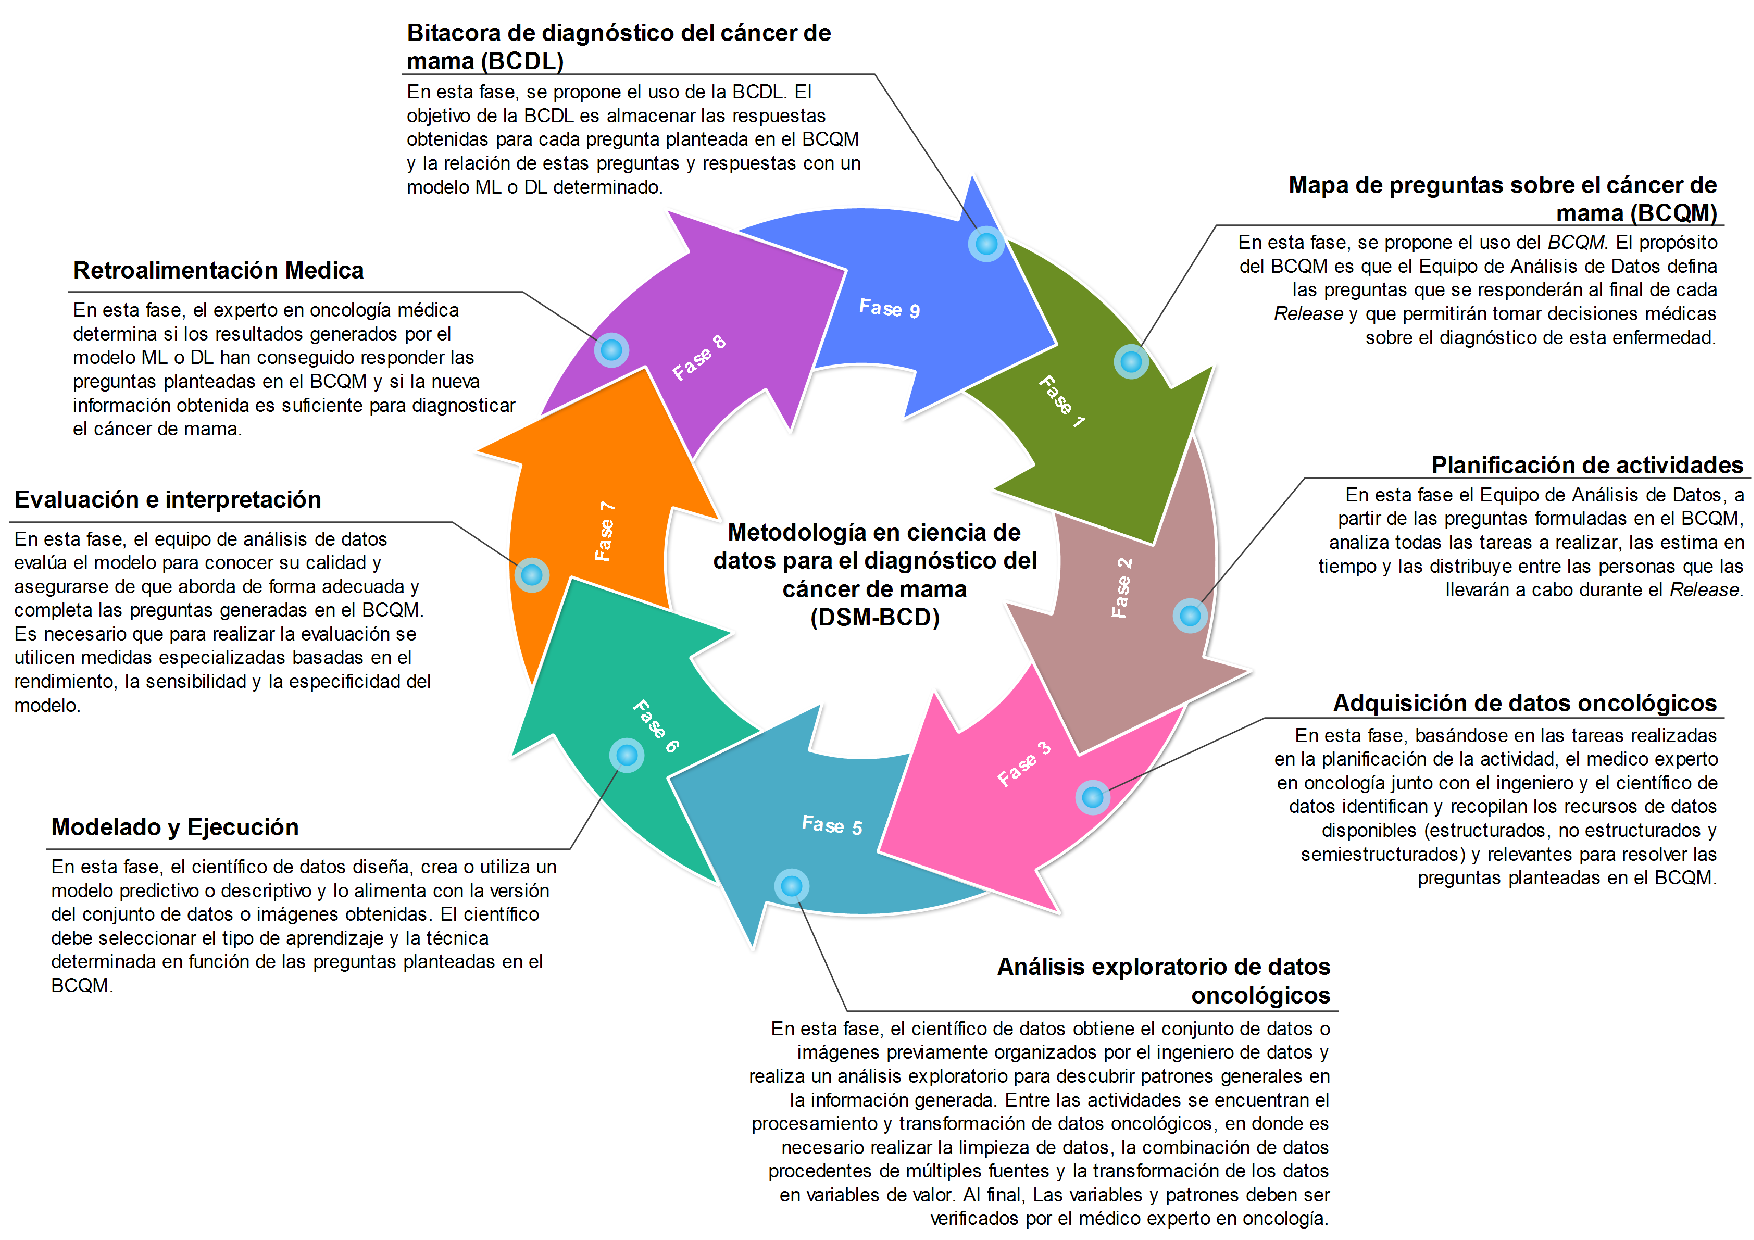
\includegraphics[width=0.9
	\linewidth]{IMAGENES/DSM-BCD_SPANISH.pdf}
	\caption{Metodología en ciencia de datos para el diagnóstico del cáncer de mama 
		(DSM-BCD)\cite{DSMBCD023}.}
	\label{DSM-BCD}
\end{figure*}

Esta metodología tiene como base el \textit{manifestó ágil} aplicado a un contexto de resultados basados en datos. Dado lo anterior \textit{DSM-BCD} no se enfoca en evaluar la precisión de las técnicas de ML y DL sino su objetivo principal es generar valor a los datos en el tiempo más corto posible para que los médicos diagnostiquen de manera ágil el cáncer de mama. Para lograrlo \textit{DSM-BCD} integra la perspicacia médica y los resultados obtenidos por las técnicas de ML y DL en una retroalimentación continúa generada en cada \textit{Release} para producir mayor eficacia en la toma de decisiones

En \textit{DSM-BCD}, se sugiere la conformación de un \textit{Equipo de análisis de datos (Data Analysis Team)}. Este equipo debe estar encabezado por el medico experto en oncología, al menos un ingeniero de datos y un científico de datos. Se recomienda que el equipo este conformado por un máximo de 5 personas para facilitar el trabajo en equipo y la comunicación interna.

Para comprender mejor el uso de DSM-BCD, se realizó un análisis descriptivo y predictivo basados en datos genéticos característicos de tumores generados por los tipos de cáncer \textit{Carcinoma ductal invasivo (IDC)} y \textit{Carcinoma lobulillar invasivo (ILC)}, en donde se logró determinar que el IDC y ILC son enfermedades molecularmente distintas con rasgos genéticos característicos, lo que proporciona información importante para la estratificación de los pacientes permitiendo realizar diagnóstico clínico ágil con precedentes para un tratamiento puntual.

\section{Fase 1: BCQM} 
En esta fase se propone el uso de un mapa de preguntas sobre el cáncer de mama (Por sus siglas en ingles Breast Cancer Question Map (BCQM)). El proposito del \textit{BCQM} es que el \textit{Data Analysis Team} defina las preguntas que serán resueltas al finalizar cada \textit{Release} y que permitirán tomar decisiones medicas con respecto al diagnostico de esta enfermedad. En la figura \ref{BCQM} se observa la estructura del BCQM.

\begin{figure}
	\centering
	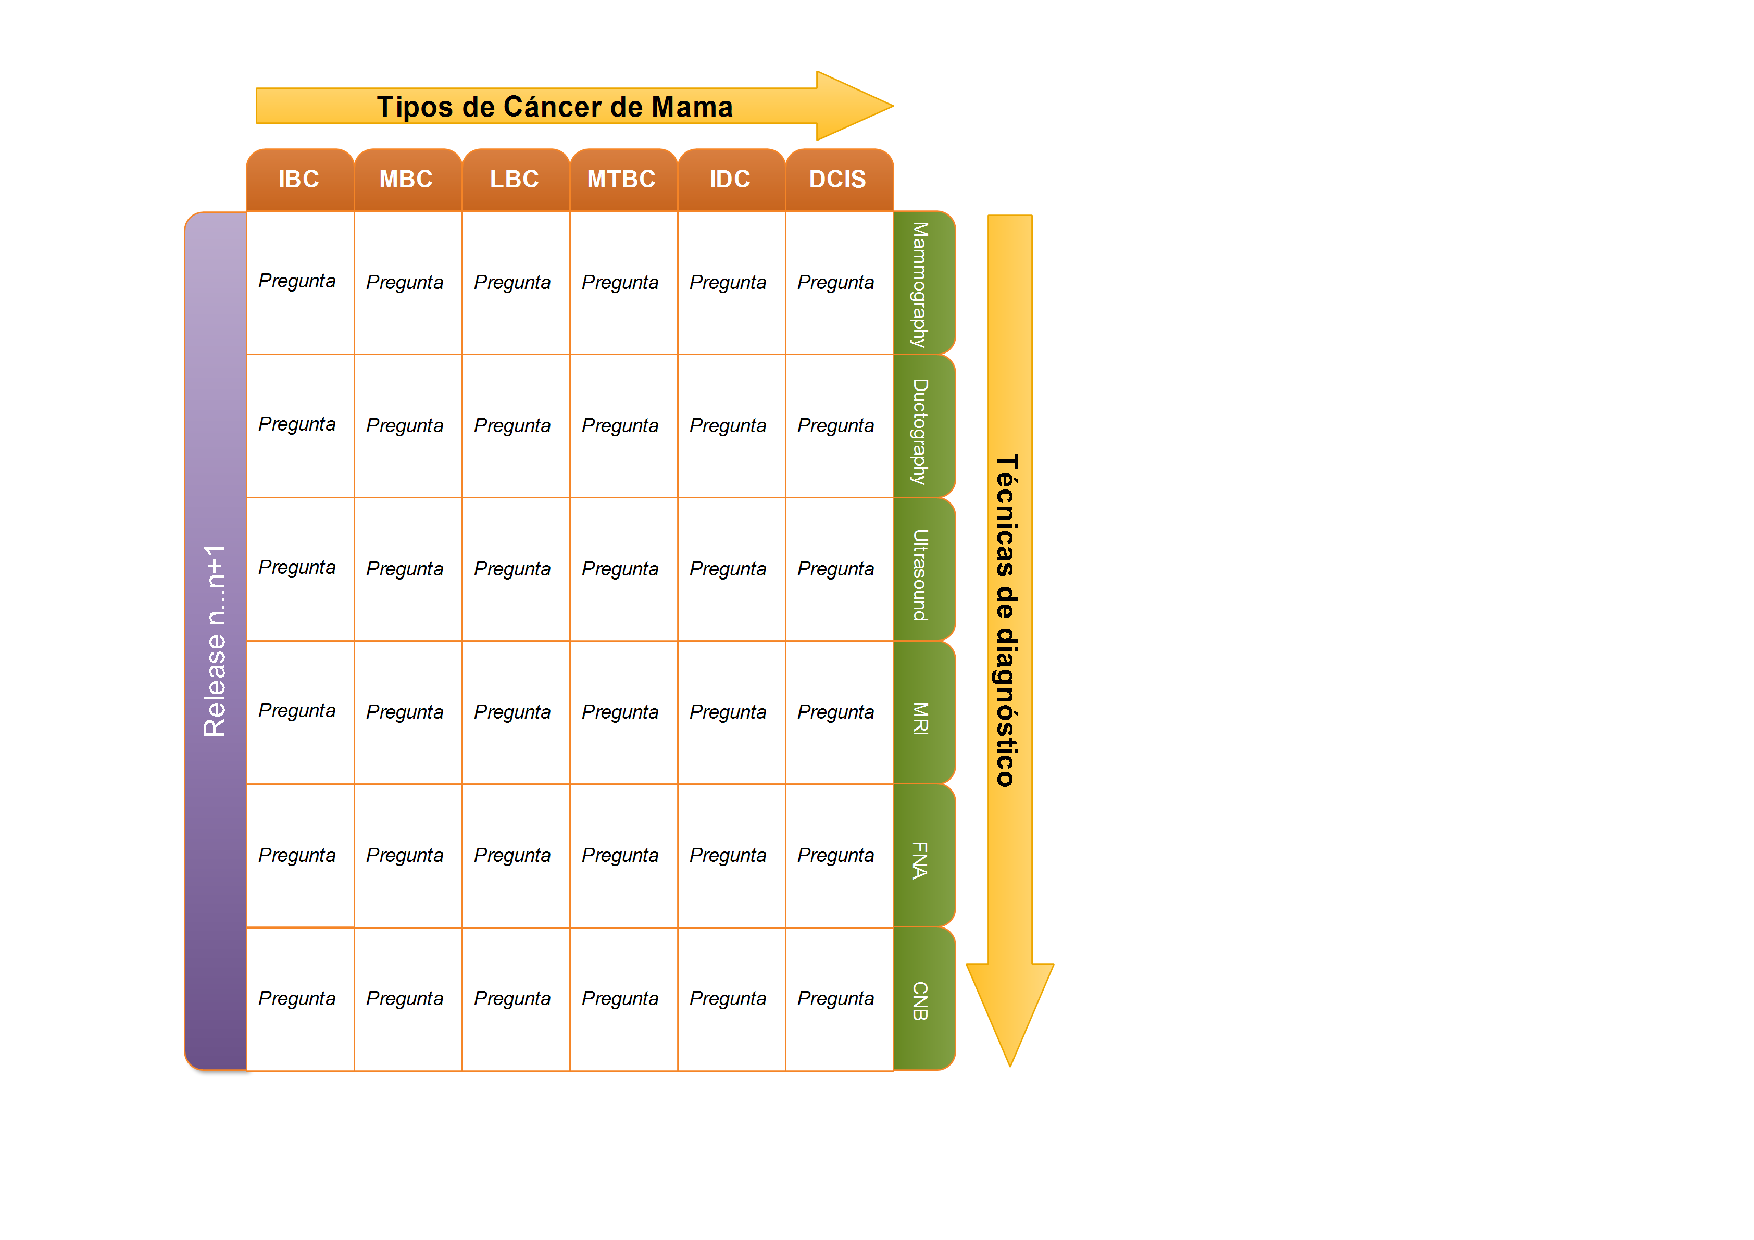
\includegraphics[width=0.8
	\linewidth]{IMAGENES/BCQM_SPANISH}
	\caption{Breast Cancer Question Map (BCQM). Aplicado a tipos de cáncer \textit{Inflamatorio (IBC)}, \textit{mucinoso (MBC)}, \textit{Lobulillar (LBC)}, \textit{Tumores mixtos (MTBC)}, \textit{Carcinoma ductal invasivo (IDC)} y \textit{Carcinoma ductal in situ (DCIS)}}
	\label{BCQM}
\end{figure}

El BCQM permite plantear preguntas relacionadas a los tipos de cáncer de mama y a las técnicas para el diagnostico de la misma. De modo que al finalizar el tiempo de cada \textit{Release}, el cual puede variar entre 1 y 4 semanas, las preguntas serán respondidas según el análisis de datos generado, y el medico podrá tomar una decisión de valor. Cabe resaltar, que es posible tener una o mas preguntas relacionadas a una técnica y a un tipo de cáncer de mama por cada \textit{Release}, razón por la cual es posible encontrar correlaciones entre las variables características de cada tipo de cáncer encontrando así patrones ocultos en los diferentes conjuntos de datos.

 Con base a lo anterior, es recomendable que se generen máximo 3 preguntas por Release, debido a que a nivel de ciencia de datos la respuesta de una sola pregunta conlleva a un proceso complejo y el objetivo principal de la metodología es generar respuestas de valor que aporten en la agilidad del diagnostico del cáncer de mama, por lo que generar una cantidad muy grande de preguntas puede generar un desperdicio de informacion en el tiempo establecido en el Release para dar una respuesta.
 
 Adicionalmente, el BCQM permite identificar a que técnica para el diagnostico de cáncer mama esta relacionada la pregunta a resolver, lo cual de antemano hace posible conocer el tipo información (imágenes o datos) y el algoritmo  ML o DL requerido para dar solución al problema. Dada la naturaleza de las preguntas, es posible  que las mismas estén relacionadas a varias técnicas de diagnostico al mismo tiempo. Así mismo, el BCQM permite definir desde la fase inicial el tipo de modelo predictivo o descriptivo según el enfoque analítico generado por la pregunta planteada. Sintetizando, el uso de BCQM facilita la comprensión del problema medico y permite identificar previamente la técnica, el tipo de información y enfoque que debe ser utilizado para el análisis de datos.  

Para este caso de estudio, se plantearon las preguntas que observan en la figura \ref{BCQ_TCGA} a partir del proyecto de carcinoma invasivo de mama denominado \textit{“Comprehensive Molecular Portraits of Invasive Lobular Breast Cancer”}\cite{Ciriello2015}, basado en el \textit {Atlas del Genoma del Cáncer (TCGA\footnote{Acrónimo de “The Cancer Genome Atlas (TCGA)”, en inglés })} cuya finalidad es catalogar cambios moleculares de importancia biológica responsables de la aparición de cáncer haciendo uso de la secuenciación genómica y la bioinformática \cite{TCGA2023}.
\begin{figure}
	\centering
	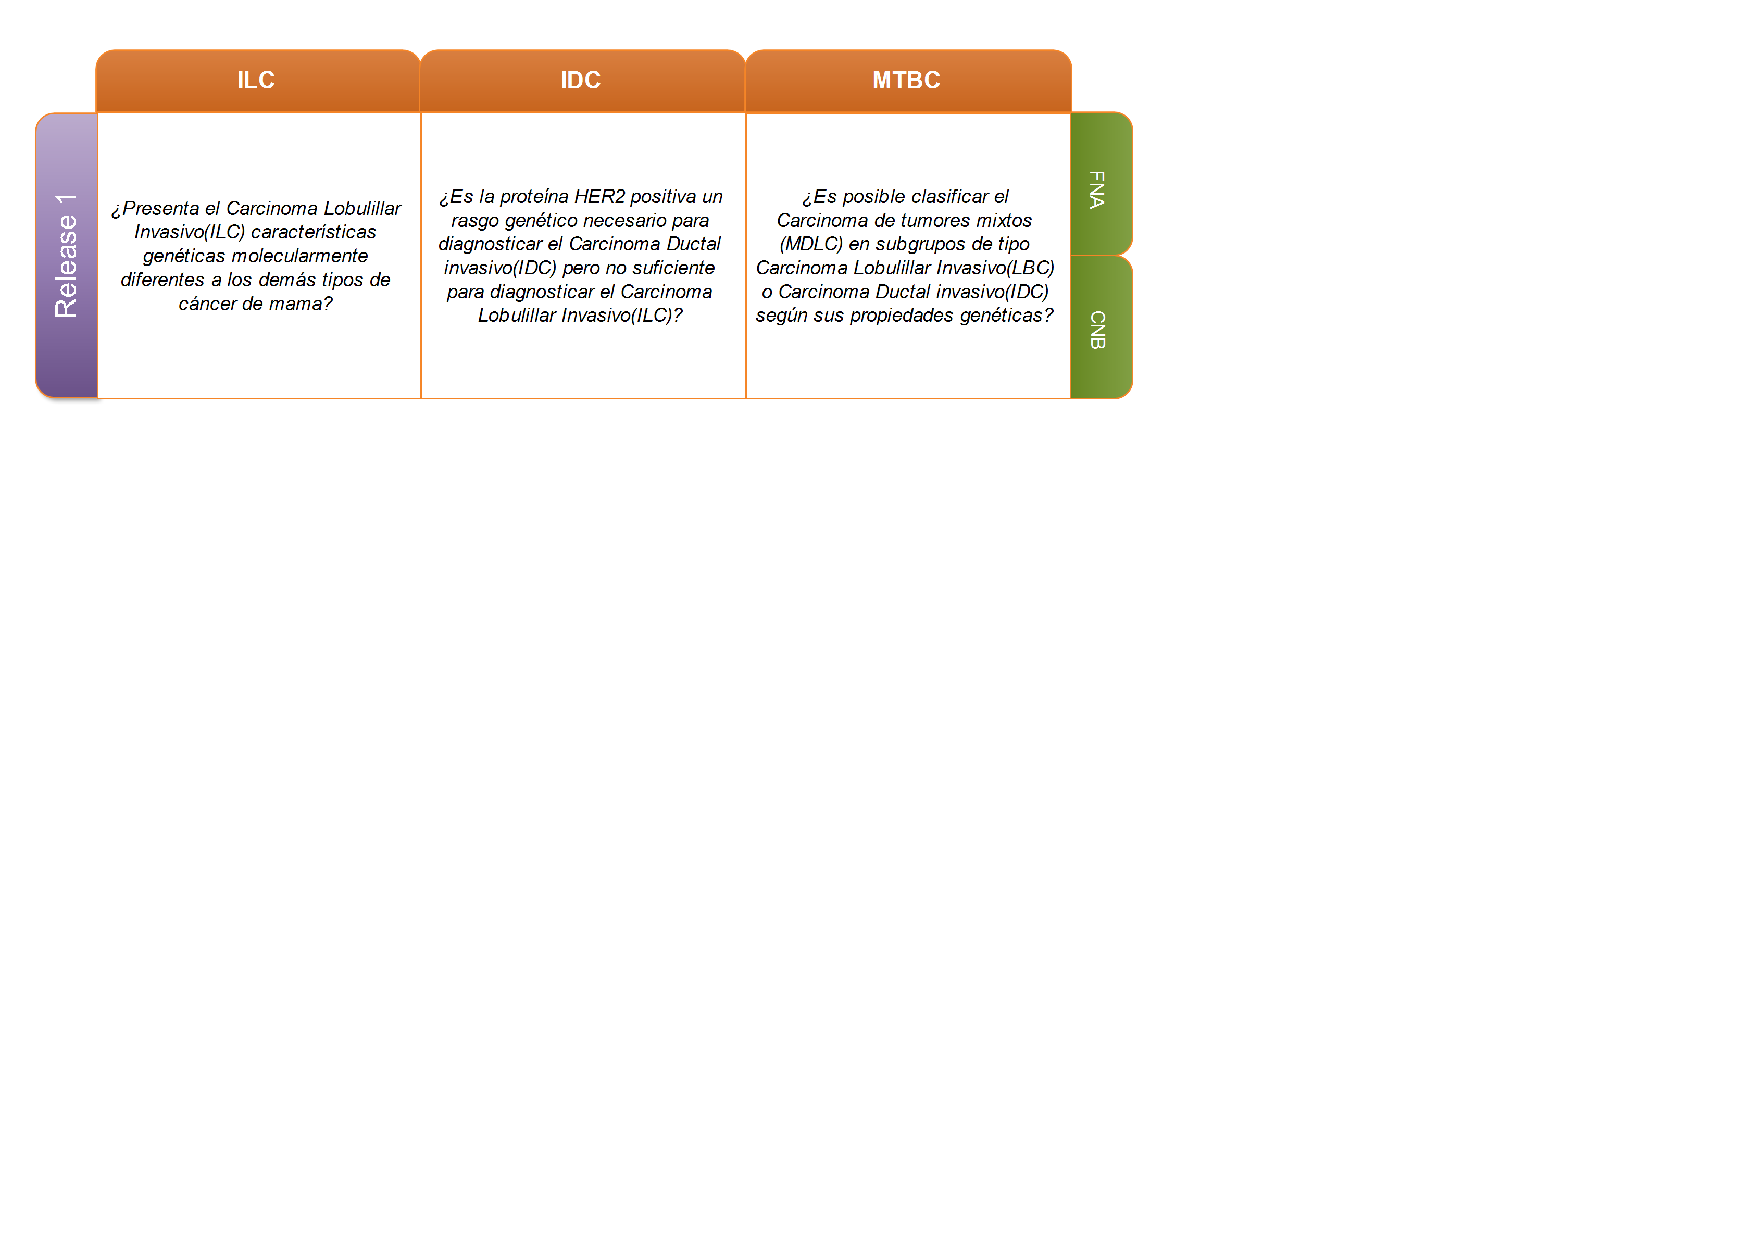
\includegraphics[width=1
	\linewidth]{IMAGENES/BCQM_TCGA}
	\caption{BCQM generado para el caso de estudio.}
	\label{BCQ_TCGA}
\end{figure}

Dadas las preguntas generadas, los tipos de cáncer de mama seleccionados son los siguientes:
\begin{itemize}[label=\HandRight]
	\item \textbf{Carcinoma Lobulillar Invasivo (LBC)}:  Este tipo de cáncer ocurre dentro del lóbulo mamario y aumenta las posibilidades de otros cánceres invasivos. 
	\item \textbf{Carcinoma Ductal Invasivo (IDC)}:Este tipo de cáncer ocurre cuando las células anormales de la mama se diseminan por los conductos conformados por los tejidos mamarios.
	\item \textbf{Tumores Mixtos (MTBC)}: Este tipo de cáncer es causado por las células anormales de los conductos y las células lobulillares, por que esta conformado por los tipos de cáncer LBC e IDC.
\end{itemize}

Con base a los tipos de cáncer de mama anteriores y a las preguntas planteadas en el BCQM que requieren informacion de índole genético, la técnica de diagnóstico mas adecuada es la \textit{Biopsia}. Dado lo anterior, en el BCQM se relacionan las biopsias que incluyen las siguientes técnicas: 

\begin{itemize}[label=\HandRight]
	\item \textbf{Biopsia por aspiración con aguja fina (FNA\footnote{Fine Needle Aspiration})}: Se usa una aguja calibre 22 de 4 cm unida a una jeringa de 10 ml. El uso de un soporte de la jeringa permite que el cirujano que toma la biopsia controle la jeringa y la aguja con una mano en tanto sitúa la masa mamaria con la mano opuesta. Tras colocar la aguja en la masa, se aspira en tanto se mueve la aguja hacia adelante y atrás dentro de la masa. La aspiración se detiene y la aguja se extrae una vez que se observa material celular en la cabeza de la aguja \cite{Brunicardi2010}. Este procedimiento quirúrgico se puede observar en la figura \ref{FNB}.
	 \begin{figure}[!htb]
	 	\centering
	 	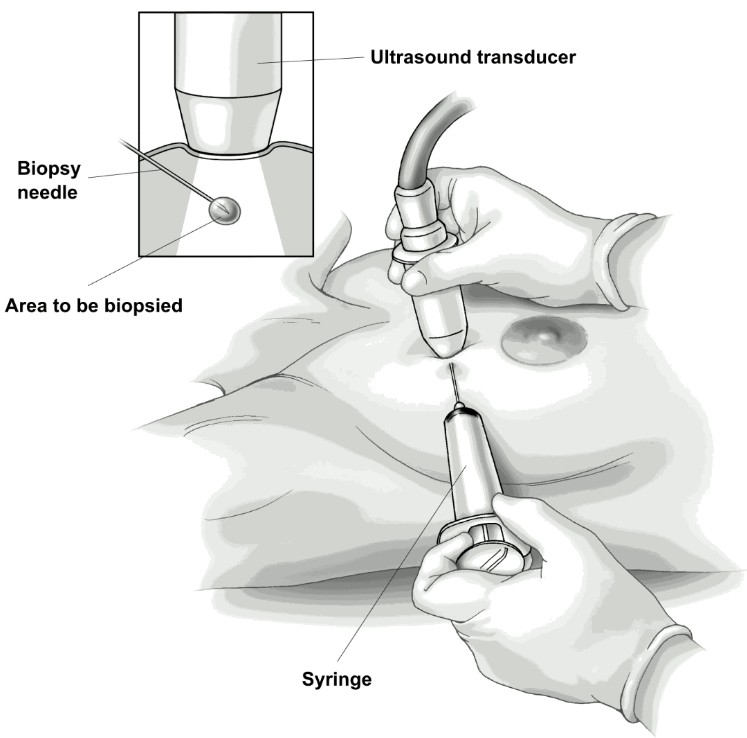
\includegraphics[width=0.5
	 	\linewidth]{IMAGENES/FNB}
	 	\caption{Aspiración con aguja fina\cite{FNB}.}
	 	\label{FNB}
	 \end{figure}	
	 \\
	
	\item \textbf{Biopsia con aguja gruesa (CNB\footnote{Core Needle Biopsy})}: Se usa en masas palpables de la mama  con una aguja calibre 14, como la Tru-Cut. También se cuenta con dispositivos automatizados. Las muestras de tejidos se colocan en formalina y luego se procesan para bloques de parafina \cite{Brunicardi2010}. Este procedimiento quirúrgico se puede observar en la figura \ref{CNB}.
	\begin{figure}[!htb]
		\centering
		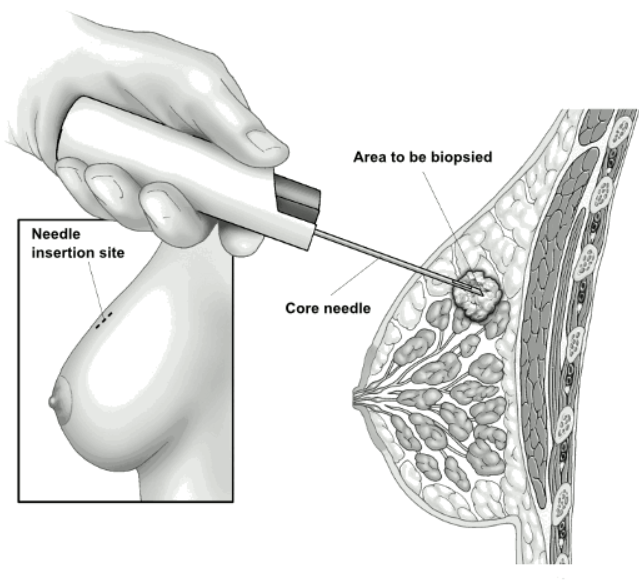
\includegraphics[width=0.5
		\linewidth]{IMAGENES/CNB}
		\caption{Biopsia con aguja gruesa\cite{CNB}.}
		\label{CNB}
	\end{figure}	
\end{itemize}

Considerando la naturaleza de la información, la técnica computacional a utilizar es \textit{Machine Learning} debido a que los datos son de origen genómico y por ende tendrán una representación simbólica con atributos cuantitativos y/o cualitativos. Cabe resaltar, que dado el origen de las preguntas, los modelos de ML a utilizar deben permitir realizar los siguientes tipos de análisis:

\begin{itemize}[label=\HandRight]
	\item \textbf{Análisis Descriptivo}:
	Este tipo de análisis se genera a partir de datos de entrada que no están etiquetados y no tienen un resultado conocido \cite{JorgeCalvo2020}.
	
	\item \textbf{Análisis Predictivo}:Este tipo de análisis se genera a partir de datos históricos reales para hacer predicciones acerca del valor de una variable o dato desconocido \cite{JorgeCalvo2020}.
\end{itemize}


\section{Fase 2: Planeación de actividades}
En esta fase el \textit{Data Analysis Team} basado en las preguntas realizadas en el BCQM analiza todas las tareas que hay que llevar a cabo, las estiman en tiempo y las distribuyen entre las personas que las van a realizar durante el \textit{Release}. Dado que el BCQM nos permite conocer de antemano el tipo de cáncer de mama y la técnica para el diagnóstico de esta enfermedad, el científico de datos con ayuda del médico puede definir el origen de datos, lo cual va a permitir conocer el tipo, cantidad y peso de la información. Dado lo anterior, es recomendable que el equipo tenga al menos un ingeniero datos, ya que él es el encargado de tomar los datos y convertirlos en información significativa para que el científico pueda realizar el respectivo análisis.  

\begin{figure}[!htb]
	\centering
	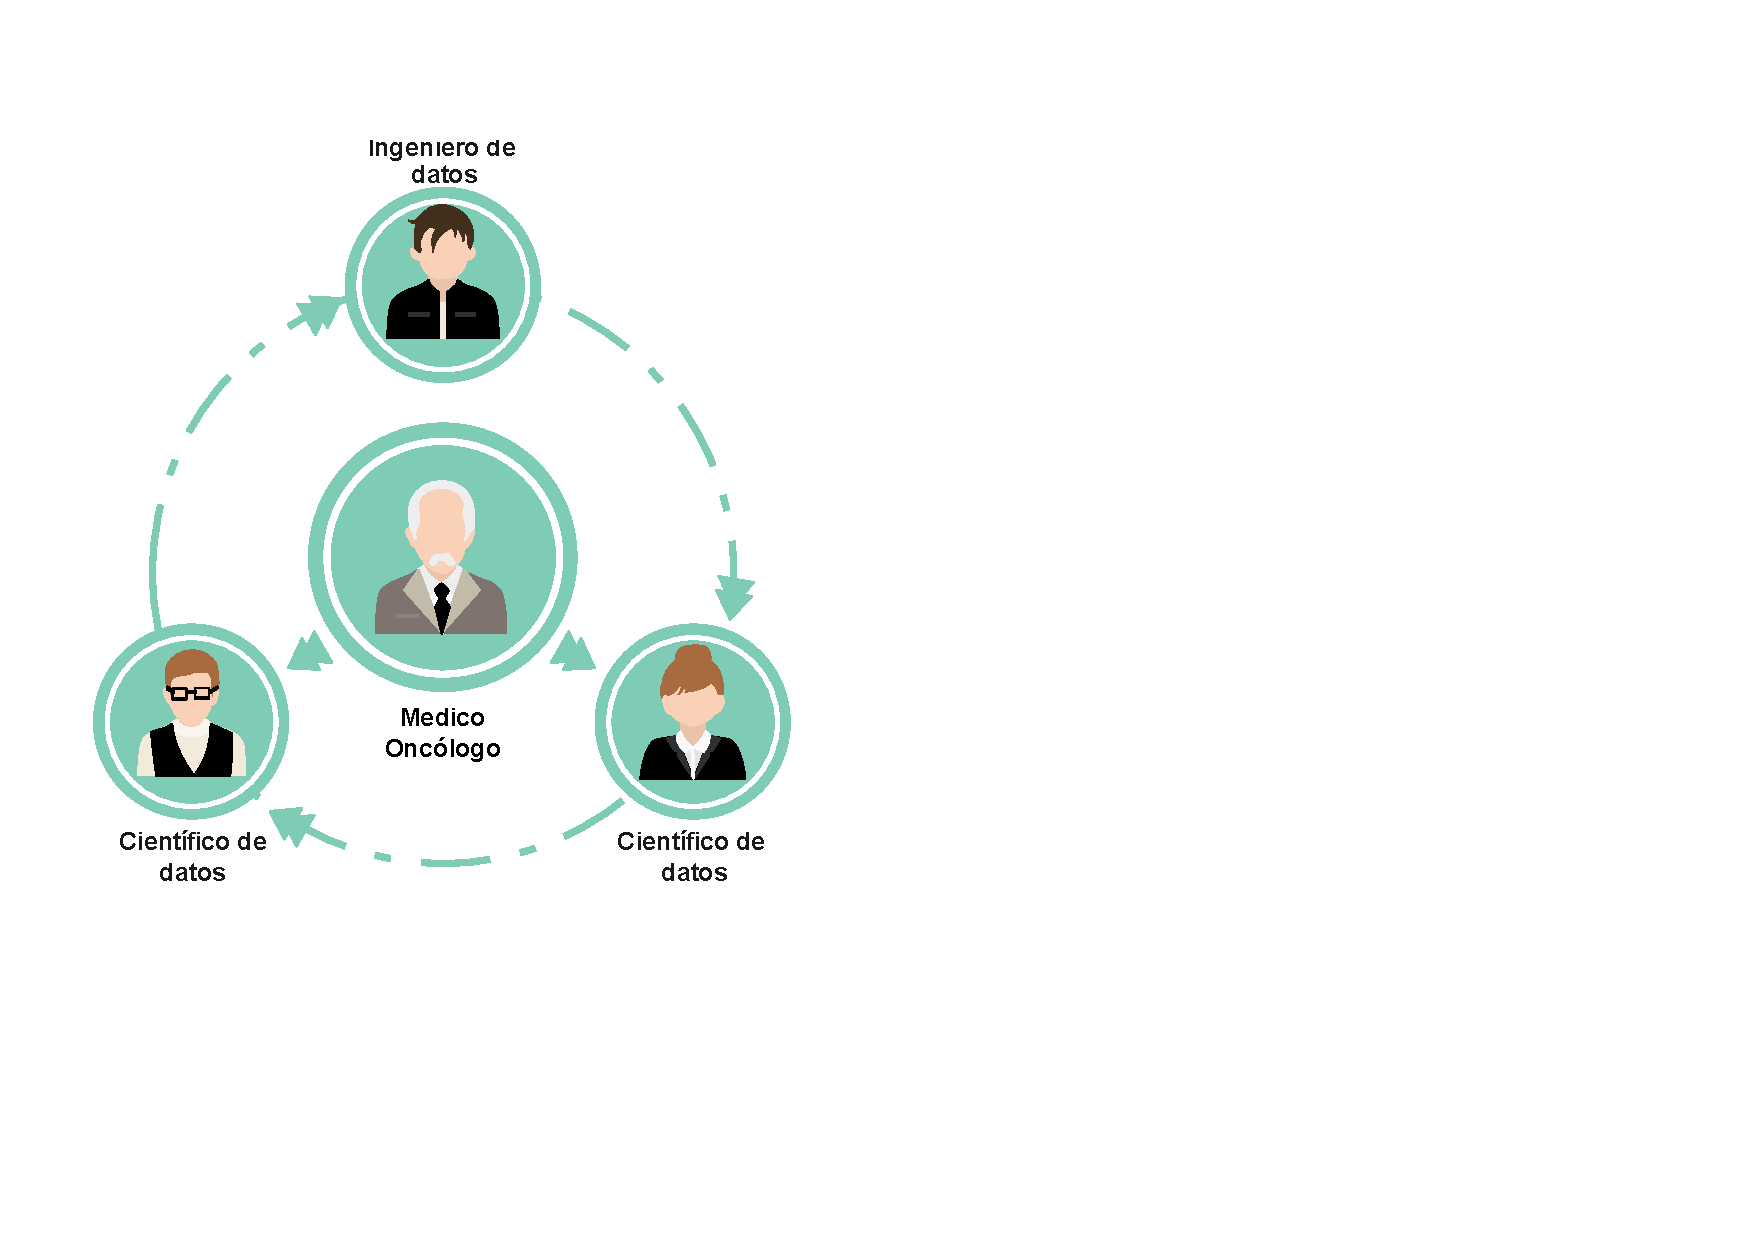
\includegraphics[width=0.36
	\linewidth]{IMAGENES/Data_Analysis_Team}
	\caption{Conformación del Data Analysis Team\cite{planning023}. }
	\label{Data_Analysis_Team}
\end{figure}

\begin{figure}[!htb]
	\centering
	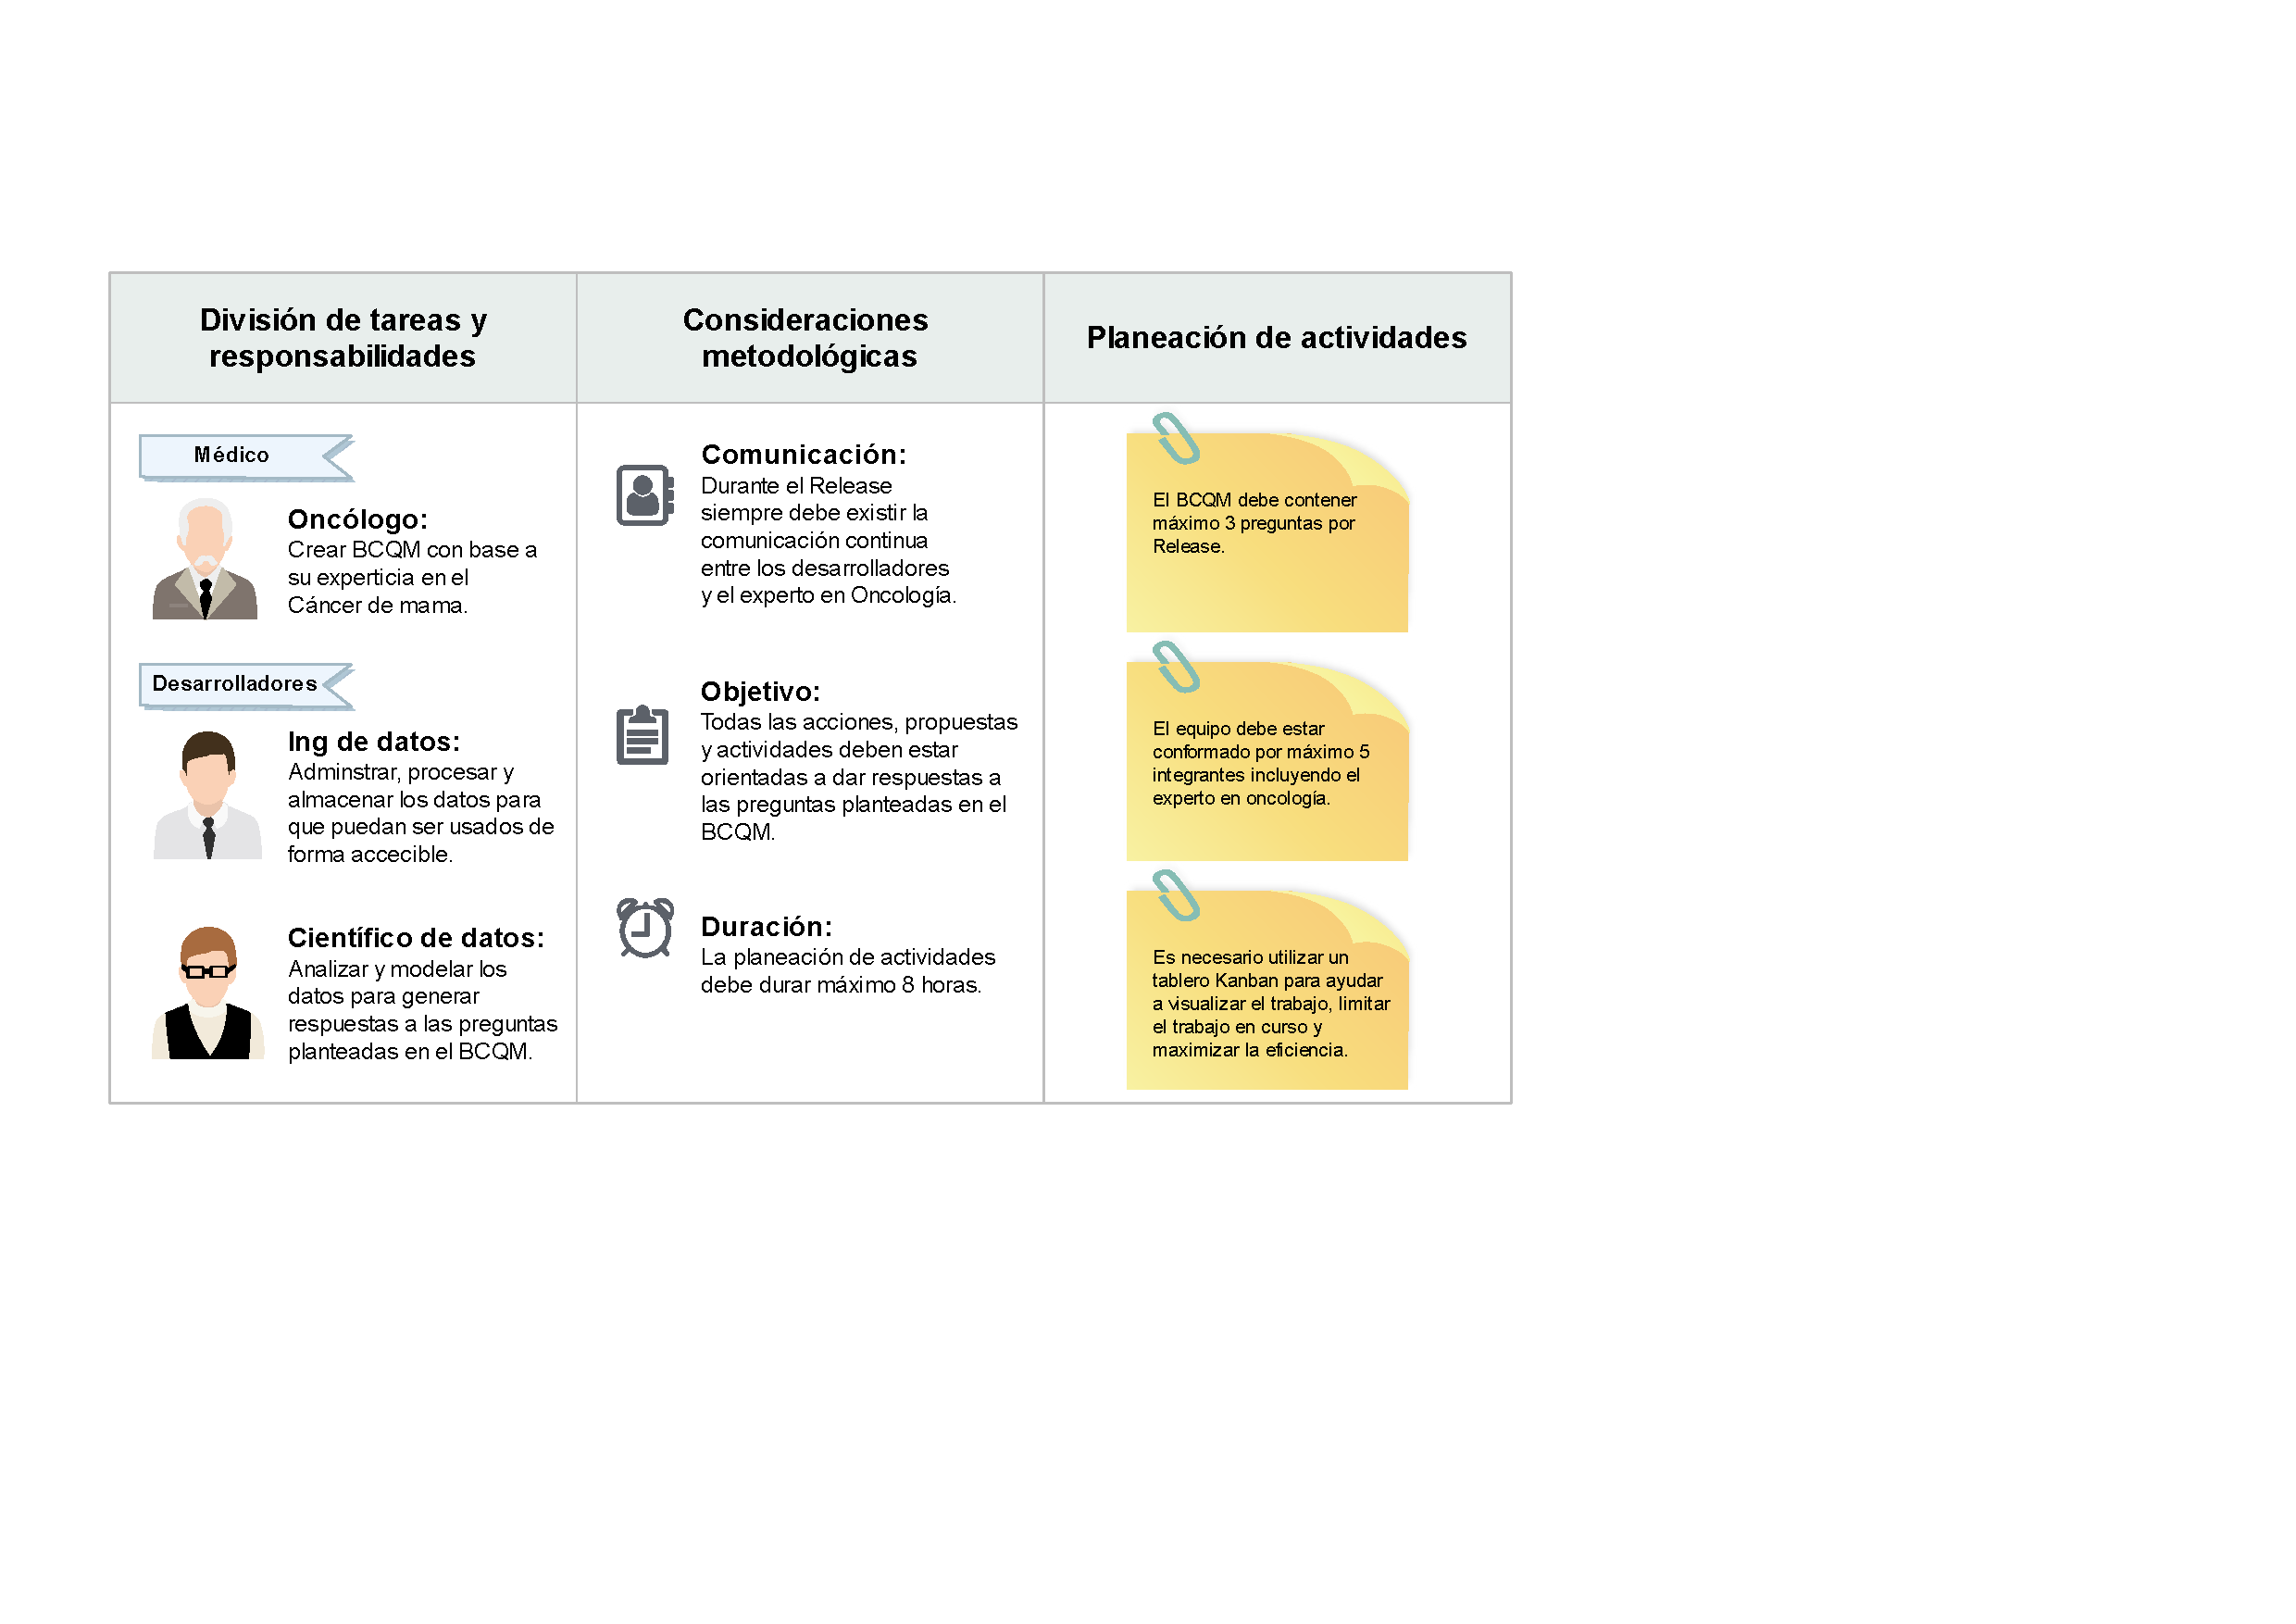
\includegraphics[width=0.68
	\linewidth]{IMAGENES/Activity_Planning}
	\caption{Planeación de actividades \cite{planning023}. }
	\label{Activity_Planning}
\end{figure}

Una vez generadas las preguntas en el BCQM es posible que varias actividades este relacionadas a varias preguntas, por lo tanto, se recomienda al \textit{Data Analysis Team} agrupar en una sola actividad las tareas a realizar para generar una mayor agilidad en la elaboración de interpretaciones y respuestas. Así mismo todas las acciones, propuestas y actividades deben estar orientadas en generar respuestas a las preguntas planteadas, siendo el principal objetivo que el experto en oncología tome una decisión de valor. Dado lo anterior, durante el Release siempre debe existir una comunicación continua y efectiva entre el equipo técnico y el experto en oncología. Finalmente, la planeación de actividades debe durar máximo 8 horas y su creación debe estar de acuerdo a las habilidades técnicas de cada participante del equipo.

Para un mayor entendimiento, basados en las 3 preguntas planteadas en el BCQM, se generó la siguiente planeación de actividades para generar respuestas basados en los datos de índole genómico responsables del desarrollo del cáncer de mama:
\begin{figure}[!htb]
	\centering
	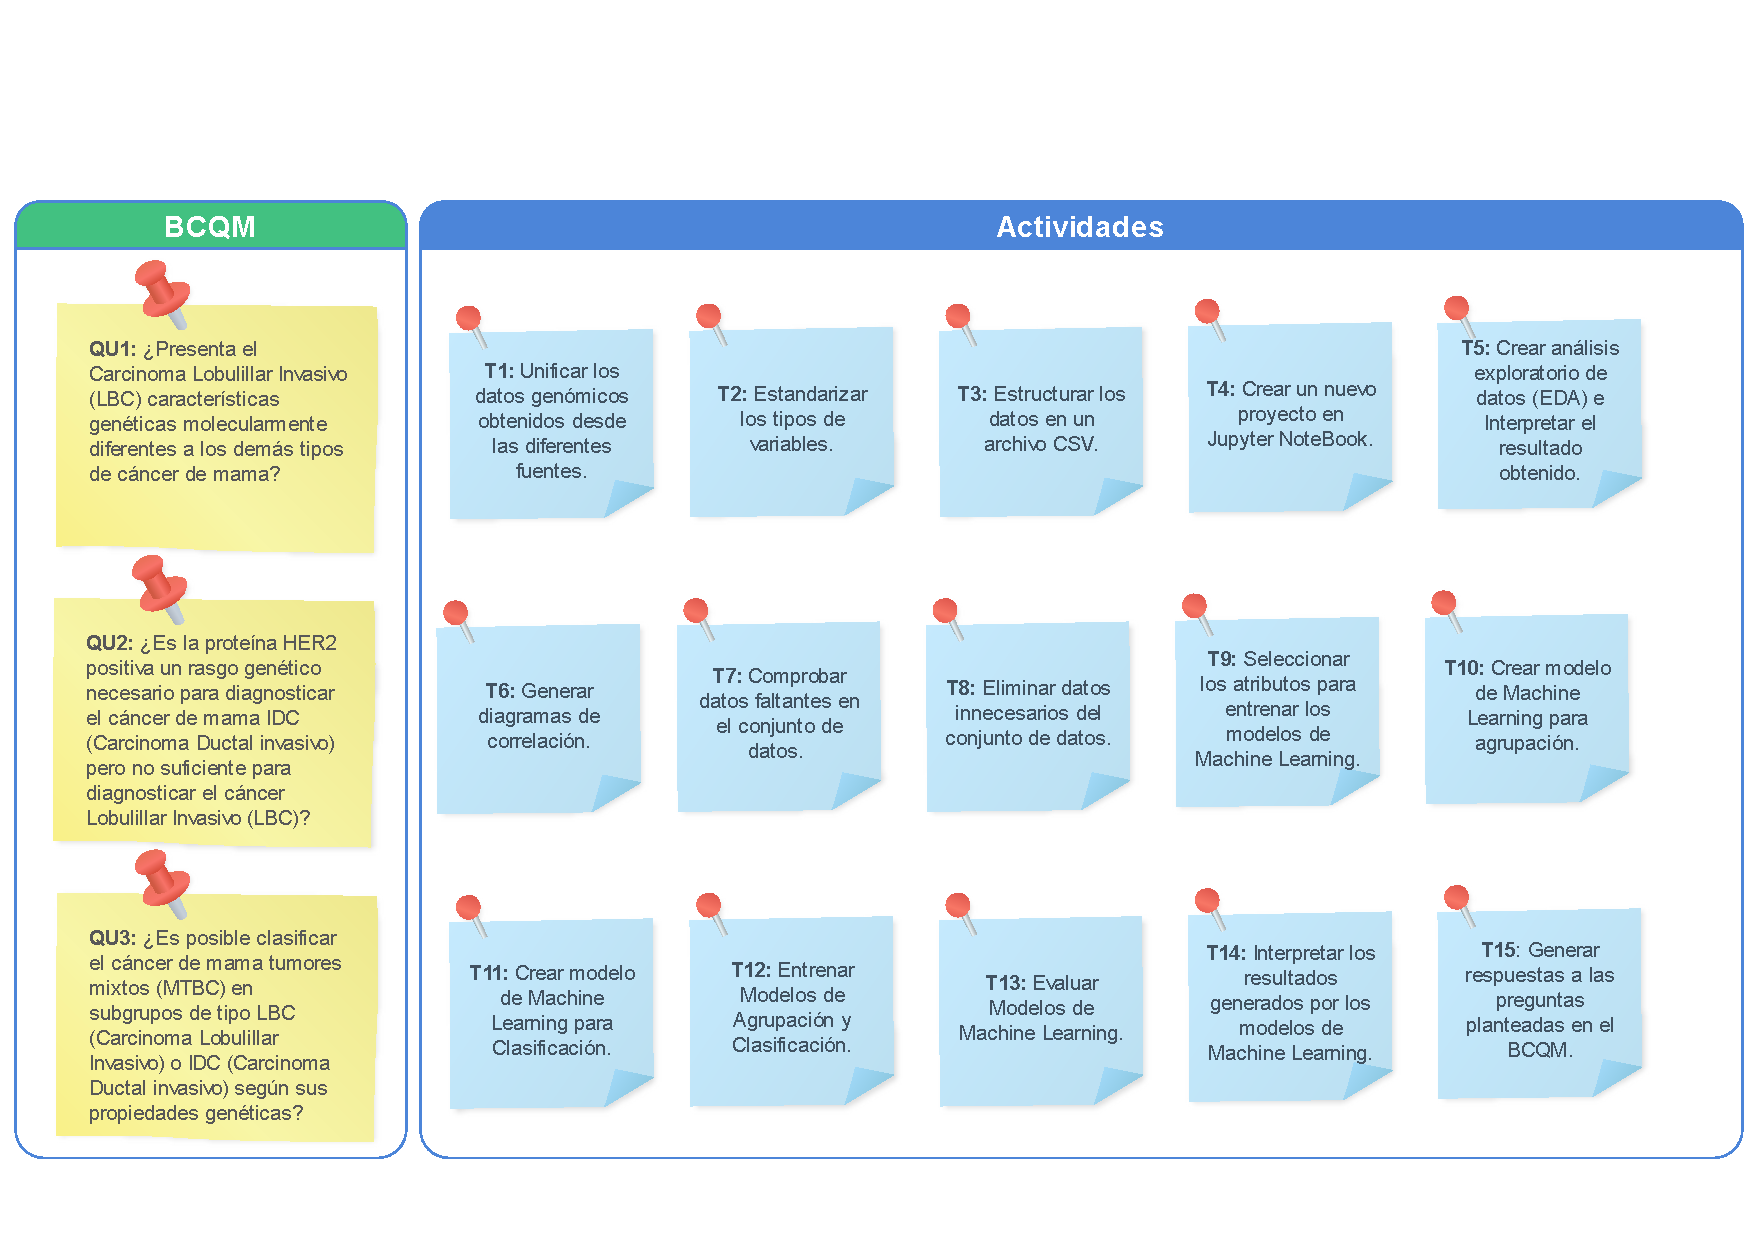
\includegraphics[width=
	\linewidth]{IMAGENES/Planning_TCGA}
	\caption{Planeación de actividades aplicada al caso de estudio\cite{planningDSM2023}.}
	\label{Activity_Planning_TCGA}
\end{figure}

\section{Fase 3: Adquisición de datos oncológicos}
En esta fase, con base a la tareas realizadas en la planeación de actividades, el medico experto en oncología junto con el ingeniero y el científico de datos identifican y reúnen los recursos de datos disponibles (estructurados, no estructurados y semiestructurados) y relevantes para solucionar las preguntas planteadas en el \textit{BCQM}. Cabe resaltar, que en la metodología \textit{\textit{DSM-BCD}} es factible tener varios conjuntos de datos o imágenes que están relacionados a un tipo de cáncer de mama y una técnica de diagnostico, por lo tanto  el \textit{Data Analysis Team} puede tener a varios científicos respondiendo preguntas diferentes en un mismo \textit{Release}. Como consecuencia, al final se pueden obtener como resultado múltiples respuestas y una posible correlación entre las diversas variables oncológicas.  Asimismo, en esta fase el \textit{Data Analysis Team} debe definir la infraestructura de datos necesaria según la cantidad de información a procesar, lo cual permitirá proyectar la escalabilidad, alcance y distribución de dicha información. 

Para este caso de estudio, se utilizaron variables genéticas características de marcadores tumorales  basados en los tipos de cáncer de mama  \textit{Carcinoma ductal invasivo (IDC)} y \textit{Carcinoma lobulillar invasivo (LBC)}. Estas variables fueron obtenidas del conjunto de datos denominado \textit{“Breast Invasive Carcinoma (TCGA, Cell 2015)”} creado a partir del proyecto de carcinoma invasivo de mama \textit{“Comprehensive Molecular Portraits of InvasiveLobular Breast Cancer”} \cite{Ciriello2015} basado en el \textit {Atlas del Genoma del Cáncer (TCGA\footnote{Acrónimo de “The Cancer Genome Atlas (TCGA)”, en inglés })} cuya finalidad es catalogar cambios moleculares de importancia biológica responsables de la aparición de cáncer haciendo uso de la secuenciación genómica y la bioinformática \cite{TCGA2023}. Los datos fueron descargados del sitio público \textit{cBioPortal} para la genómica del cáncer  (\url{https://www.cbioportal.org/study/summary?id=brca_tcga_pub2015}). 

Cabe resaltar, que el conjunto de datos contiene un total de 817 muestras de tumores de mama que  se perfilaron con 6 plataformas moleculares: Análisis del número de copias somáticas basado en array, Secuenciación del exoma completo, perfil de metilación del ADN basado en array, secuenciación del ARN mensajero, Secuenciación de microARN (miARN) y Array de proteínas en fase inversa (RPPA), como se ha descrito previamente en \cite{Bass2014}. Un comité de patología revisó y clasificó todos los tumores en 490 IDC, 127 LBC, 88 casos con características mixtas de IDC y LBC, y 112 con otras histologías. Este conjunto de datos consta de un tamaño de $818$ filas y $110$ columnas. Las variables se describen en la tabla \ref{brca_tcga_pub2015_clinical_data}. 

\begin{table*} [!htb]
	\footnotesize
	\begin{threeparttable}
		\caption{Conjunto de datos del Carcinoma invasivo de mama (TCGA, Cell 2015).}
		\label{brca_tcga_pub2015_clinical_data}
		\begin{tabular}{p{1cm} p{4cm} p{10cm}} \toprule	
			\begin{center}$N$\end{center}   
			&\begin{center}Variable\end{center}             
			&\begin{center}Descripción\end{center}      
			\\ \hline	1	&	Study ID	&	Código de identificación del estudio
			\\ \hline	2	&	Patient ID	&	Código de identificación del paciente
			\\ \hline	3	&	Sample ID	&	Código de identificación de la muestra
			\\ \hline	4	&	Diagnosis Age	&	Edad a la que se diagnosticó por primera vez una afección o enfermedad
			\\ \hline	5	&	American Joint Committee on Cancer Metastasis Stage Code	&	Código para representar la ausencia o presencia definida de diseminación a distancia o metástasis (M) a localizaciones a través de canales vasculares o linfáticos más allá de los ganglios linfáticos regionales, utilizando los criterios establecidos por el Comité Conjunto Americano del Cáncer (AJCC)
			\\ \hline	6	&	Neoplasm Disease Lymph Node Stage American Joint Committee on Cancer Code	&	Los códigos que representan el estadio del cáncer en función de los ganglios presentes (estadio N) según criterios basados en múltiples ediciones del Manual de Estadificación del Cáncer de la AJCC
			\\ \hline	7	&	Neoplasm Disease Stage American Joint Committee on Cancer Code	&	Estadio de la extensión de un cáncer, especialmente si la enfermedad se ha propagado desde el sitio original a otras partes del cuerpo según los criterios de estadificación del AJCC
			\\ \hline	8	&	American Joint Committee on Cancer Publication Version Type	&	Versión o edición del American Joint Committee on Cancer Cancer Staging Handbooks, publicación del grupo formado con el propósito de desarrollar un sistema de estadificación clínica del cáncer que sea aceptable para la profesión médica estadounidense y compatible con otras clasificaciones aceptadas
			\\ \hline	9	&	American Joint Committee on Cancer Tumor Stage Code	&	Código de T patológico (tumor primario) para definir el tamaño o la extensión contigua del tumor primario (T), utilizando los criterios de estadificación del AJCC
			\\ \hline	10	&	Brachytherapy first reference point administered total dose	&	Primer punto de referencia dosis total administrada en la Braquiterapia
			\\ \hline	11	&	Cancer Type	&	Tipo de cáncer
			\\ \hline	12	&	Cancer Type Detailed	&	Detalle del tipo de cáncer
			\\ \hline	13	&	Cent17 Copy Number	&	Intervalo de resultados de la señal del cromosoma 17 del procedimiento de diagnóstico de hibridación in situ con fluorescencia.
			\\ \hline	14	&	Birth from Initial Pathologic Diagnosis Date	&	Intervalo de tiempo desde la fecha de nacimiento de una persona hasta la fecha del diagnóstico patológico inicial, representado como un número calculado de días.
			\\ \hline	15	&	Days to Sample Collection.	&	Días para la recolección de muestras
			\\ \hline	16	&	Death from Initial Pathologic Diagnosis Date	&	Intervalo de tiempo desde la fecha de muerte de una persona hasta la fecha del diagnóstico patológico inicial, representado como un número calculado de días.
			\\ \hline	17	&	Last Alive Less Initial Pathologic Diagnosis Date Calculated Day Value	&	Intervalo de tiempo desde el último día en que se sabe que una persona está viva hasta la fecha del diagnóstico patológico inicial, representado como un número calculado de días.
			\\ \hline	18	&	Days to Last Followup	&	Intervalo de tiempo desde la fecha del último seguimiento hasta la fecha del diagnóstico patológico inicial, representado como un número calculado de días.
			\\ \hline	19	&	Disease Free (Months)	&	Sin enfermedad (meses)
			\\ \hline	20	&	Disease Free Status	&	Estado libre de enfermedad
			\\ \hline	21	&	Disease code	&	Código de la enfermedad
			\\ \hline	22	&	ER positivity scale other	&	Escala de medición de otro receptor de estrógeno de hallazgo positivo
			\\ \hline	23	&	ER positivity scale used	&	Escala de hallazgo ER positivo de inmunohistoquímica de carcinoma de mama
			\\ \hline	24	&	ER Status By IHC	&	Estado del receptor de progesterona del carcinoma de mama
			\\ \hline
		\end{tabular}
	\end{threeparttable}
\end{table*}

\begin{table*} [!htb]
	\footnotesize
	\begin{threeparttable}
		\begin{tabular}{p{1cm} p{4cm} p{10cm}}         
			\\ \hline	25	&	ER Status IHC Percent Positive	&	Nivel de receptor de progesterona categoría de porcentaje celular
			\\ \hline	26	&	Ethnicity Category	&	Información sobre el origen étnico.
			\\ \hline	27	&	First surgical procedure other	&	Propósito del procedimiento quirúrgico
			\\ \hline	28	&	Form completion date	&	Fecha de finalización del formulario
			\\ \hline	29	&	Fraction Genome Altered	&	Fracción de genoma alterado
			\\ \hline	30	&	HER2 and cent17 cells count	&	HER2 neu y centrómero 17 número de copia análisis entrada total número recuento
			\\ \hline	31	&	HER2 and cent17 scale other	&	HER2 y centrómero 17 resultados positivos otra escala de medición
			\\ \hline	32	&	HER2 cent17 ratio	&	Valor de la relación de señal del cromosoma 17 de HER2 neu
			\\ \hline	33	&	HER2 copy number	&	Número total de entrada de análisis de copia de carcinoma de mama HER2 neu
			\\ \hline	34	&	HER2 fish method	&	Método de cálculo de hibridación in situ de fluorescencia de HER2 erbb pos
			\\ \hline	35	&	HER2 fish status	&	Procedimiento de laboratorio tipo de resultado híbrido in situ HER2 neu
			\\ \hline	36	&	HER2 ihc percent positive	& Porcentaje de HER2 ihc positivo
			\\ \hline	37	&	HER2 ihc score	&	Resultado del nivel de inmunohistoquímica HER2
			\\ \hline	38	&	HER2 positivity method text	&	Método de positividad HER2
			\\ \hline	39	&	HER2 positivity scale other	&	Otra medida escala pos hallazgo HER2 erbb2 
			\\ \hline	40	&	Neoplasm Histologic Type Name	&	Término que designa el patrón estructural de las células cancerosas utilizado para definir un diagnóstico microscópico.
			\\ \hline	41	&	Tumor Other Histologic Subtype	&	Subtipo histológico de un tumor o el diagnóstico mixto que es diferente de las opciones especificadas anteriormente.
			\\ \hline	42	&	Neoadjuvant Therapy Type Administered Prior To Resection Text	&	Término para describir el historial de tratamiento neoadyuvante del paciente y el tipo de tratamiento administrado antes de la resección del tumor.
			\\ \hline	43	&	Prior Cancer Diagnosis Occurence	&	Término para describir los antecedentes de diagnóstico previo de cáncer del paciente y la ubicación espacial de cualquier aparición previa de cáncer.
			\\ \hline	44	&	ICD-10 Classification	&	Decima revisión de la Clasificación Estadística Internacional de Enfermedades y Problemas Relacionados con la Salud.
			\\ \hline	45	&	International Classification of Diseases for Oncology, Third Edition ICD-O-3 Histology Code	&	Tercera edición de la Clasificación Internacional de Enfermedades Oncológicas, publicada en 2000, utilizada principalmente en los registros de tumores y cáncer para codificar la localización (topografía) y la histología (morfología) de las neoplasias. Estudio de la estructura de las células y su disposición para constituir tejidos y, finalmente, la asociación entre éstos para formar órganos. En patología, proceso microscópico de identificación de las características morfológicas normales y anormales de los tejidos mediante el empleo de diversas tinciones citoquímicas e inmunocitoquímicas.
			\\ \hline	46	&	International Classification of Diseases for Oncology, Third Edition ICD-O-3 Site Code	&	Tercera edición de la Clasificación Internacional de Enfermedades Oncológicas, publicada en 2000, utilizada principalmente en los registros de tumores y cáncer para codificar la localización (topografía) y la histología (morfología) de las neoplasias. Sistema de categorías numeradas para la representación de datos.
			\\ \hline	47	&	IHC-HER2	&	Término que designa el estado de la prueba IHC-HER2
			\\ \hline	48	&	IHC Score	&	Puntuación IHC
			\\ \hline	49	&	Informed consent verified	&	Consentimiento informado verificado
			\\ \hline	50	&	Year Cancer Initial Diagnosis	&	Año del diagnóstico patológico inicial de cáncer de un individuo
			\\ \hline	51	&	Is FFPE	&	Si la muestra es de tejido fijado con formalina e incrustado en parafina (FFPE)
			\\ \hline
		\end{tabular}
	\end{threeparttable}
\end{table*}

\begin{table*} [!htb]
	\footnotesize
	\begin{threeparttable}
		\begin{tabular}{p{1cm} p{4cm} p{10cm}}
			\\ \hline	52	&	Primary Lymph Node Presentation Assessment Ind-3	&	Término que indica si se realizó una evaluación de los ganglios linfáticos en la presentación primaria de la enfermedad.
			\\ \hline	53	&	Positive Finding Lymph Node Hematoxylin and Eosin Staining Microscopy Count	&	Recuento de ganglios linfáticos positivos identificados mediante microscopía óptica con tinción de hematoxilina y eosina (H\&E).
			\\ \hline	54	&	Positive Finding Lymph Node Keratin Immunohistochemistry Staining Method Count	&	Recuento de ganglios linfáticos positivos identificados a través del método de tinción de inmunohistoquímica (IHC) de queratina
			\\ \hline	55	&	Lymph Node(s) Examined Number	&	Número total de ganglios linfáticos extirpados y evaluados patológicamente para la enfermedad
			\\ \hline	56	&	Margin status reexcision	&	Estado de los márgenes de la cirugía del cáncer de mama
			\\ \hline	57	&	Menopause Status	&	Estado de la menopausia de una mujer, el cese permanente de la menstruación, generalmente definido por 6 a 12 meses de amenorrea.
			\\ \hline	58	&	Metastatic Site	&	Localización anatómica a la que se ha extendido el cáncer
			\\ \hline	59	&	Metastatic Site Other	&	Otra localización anatómica a la que se ha extendido el cáncer
			\\ \hline	60	&	Metastatic tumor indicator	&	Presencia de metástasis
			\\ \hline	61	&	First Pathologic Diagnosis Biospecimen Acquisition Method Type	&	Nombre del procedimiento para asegurar el tejido utilizado para el diagnóstico patológico original
			\\ \hline	62	&	First Pathologic Diagnosis Biospecimen Acquisition Other Method Type	&	Método utilizado para obtener tejido para un diagnóstico patológico original que es diferente de otros métodos identificados
			\\ \hline	63	&	Micromet detection by ihc	&	Detección Micromet por ihc
			\\ \hline	64	&	Mutation Count	&	Recuento de mutaciones
			\\ \hline	65	&	New Neoplasm Event Post Initial Therapy Indicator	&	Indicador para identificar si un paciente ha tenido un nuevo evento tumoral después del tratamiento inicial
			\\ \hline	66	&	Nte cent 17 HER2 ratio	&	Valor de la relación señal HER2 neu cromosoma 17 en el carcinoma metastásico de mama 
			\\ \hline	67	&	Nte er ihc intensity score	&	Carcinoma metastásico de mama inmunohistoquímica con puntuación de celulas con ER positivo
			\\ \hline	68	&	Nte er status	&	Estado del receptor de estrógenos del carcinoma metastásico de mama
			\\ \hline	69	&	Nte er status ihc positive	&	Categoría porcentual de células de carcinoma de mama metastásico con nivel de receptores de estrógenos
			\\ \hline	70	&	Nte HER2 fish status	&	Tipo de resultado de hibridación in situ de HER2 neu de procedimiento de laboratorio de carcinoma de mama metastásico
			\\ \hline	71	&	Nte HER2 positivity ihc score	&	Resultado del nivel de inmunohistoquímica erbb2 de carcinoma de mama metastásico
			\\ \hline	72	&	Nte HER2 status	&	Término que indica si se realizó el proceso de laboratorio de carcinoma de mama metastásico estado del receptor de inmunohistoquímica HER2 neu
			\\ \hline	73	&	Nte HER2 status ihc positive	&	Porcentaje de células Carcinoma de mama metastásico HER2 erbb positivos 
			\\ \hline	74	&	Nte pr ihc intensity score	&	Puntuación de intensidad Nte pr ihc
			\\ \hline	75	&	Nte pr status by ihc	&	Estado del receptor de progesterona del carcinoma de mama metastásico
			\\ \hline	76	&	Nte pr status ihc positive	&	Porcentaje de células de nivel de receptor de progesterona de carcinoma de mama metastásico
			\\ \hline	77	&	Oct embedded	&	Término que indica si se realizón una incrustación OCT
			\\ \hline	78	&	Oncotree Code	&	Código del tipo de cancer en formato Oncotree para cBioPortal
			\\ \hline	79	&	Overall Survival (Months)	&	Supervivencia general (meses)
			\\ \hline	80	&	Overall Survival Status	&	Estado de supervivencia global del paciente.
			\\ \hline	81	&	Other Patient ID	&	Otro código de identificación del paciente
			\\ \hline
		\end{tabular}
	\end{threeparttable}
\end{table*}

\begin{table*} [!htb]
	\footnotesize
	\begin{threeparttable}
		\begin{tabular}{p{1cm} p{4cm} p{10cm}}
			\\ \hline	82	&	Other Sample ID	&	Otro código de identificación de la muestra
			\\ \hline	83	&	Pathology Report File Name	&	Nombre del archivo del informe de patología
			\\ \hline	84	&	Disease Surgical Margin Status	&	Resultados concluyentes tras el examen de los márgenes del tejido para detectar la presencia de enfermedad
			\\ \hline	85	&	Adjuvant Postoperative Pharmaceutical Therapy Administered Indicator	&	Término para indicar si el paciente tuvo o no terapia farmacéutica.
			\\ \hline	86	&	Primary Tumor Site	&	Sitio del tumor para identificar la subdivisión de órganos en un individuo con cáncer
			\\ \hline	87	&	Project code	&	Código de proyecto
			\\ \hline	88	&	Tissue Prospective Collection Indicator	&	Indicador de recolección prospectiva de tejido
			\\ \hline	89	&	PR positivity define method	&	Método utilizado para definir PR positiva
			\\ \hline	90	&	PR positivity ihc intensity score	&	Puntuación de intensidad ihc positiva de PR
			\\ \hline	91	&	PR positivity scale other	&	Otra medida de Porcentaje positivo del receptor de progesterona
			\\ \hline	92	&	PR positivity scale used	&	Escala de inmunohistoquímica para el hallazgo de receptores de progesterona positiva en el  carcinoma de mama
			\\ \hline	93	&	PR status by ihc	&	Estado del receptor de progesterona del carcinoma de mama
			\\ \hline	94	&	PR status ihc percent positive	&	Categoría de porcentaje celular del nivel del receptor de progesterona
			\\ \hline	95	&	Race Category	&	Información sobre la raza
			\\ \hline	96	&	Did patient start adjuvant postoperative radiotherapy?	&	Término para indicar si el paciente inició radioterapia postoperatoria adyuvante.
			\\ \hline	97	&	Tissue Retrospective Collection Indicator	&	Término para indicar el marco de tiempo de obtención de tejido, identificando si el tejido fue obtenido y almacenado antes del inicio del proyecto.
			\\ \hline	98	&	Number of Samples Per Patient	&	Número de muestras por paciente
			\\ \hline	99	&	Sample Type	&	Tipo de muestra
			\\ \hline	100	&	Sex	&	Sexo del paciente
			\\ \hline	101	&	Somatic Status	&	Estado somático
			\\ \hline	102	&	Staging System	&	Sistema de estadificación
			\\ \hline	103	&	Staging System\_1	&	Otro sistema de estadificación
			\\ \hline	104	&	Surgery for positive margins	&	Nombre del procedimiento quirúrgico primario de carcinoma de mama
			\\ \hline	105	&	Surgery for positive margins other	&	Nombre del procedimiento quirúrgico para márgenes positivos
			\\ \hline	106	&	Surgical procedure first	&	Nombre del procedimiento quirúrgico de carcinoma de mama
			\\ \hline	107	&	Tissue Source Site	&	Sitio fuente recopilado de la muestra (tejido, células o sangre) y metadatos clínicos que luego se envían al recurso principal de bioespecímenes.
			\\ \hline	108	&	TMB (nonsynonymous)	&	Número total de mutaciones (cambios) que se encuentran en el ADN de las células cancerosas
			\\ \hline	109	&	Person Neoplasm Status	&	El estado o condición de la neoplasia de un individuo en un momento determinado
			\\ \hline	110	&	Tumor Disease Anatomic Site	&	Término que describe el sitio anatómico del tumor o enfermedad
			\\ \hline
		\end{tabular}
	\end{threeparttable}
\end{table*}


\section{Fase 4: Análisis Exploratorio de datos oncológicos}

En esta fase, el científico de datos obtiene el conjunto de datos o imágenes que fueron organizados previamente por el ingeniero de datos y realiza un \textit{Análisis exploratorio de datos} para descubrir patrones generales en la información generada. Cabe resaltar, que en esta fase el acompañamiento del medico experto en oncología es de vital importancia, ya que los datos o imágenes que van ser explorados por el científico pueden contener variables que pueden tener o no un valor significativo para el experto, ayudando así a determinar si el análisis planteado para responder la pregunta va o no por un buen camino, de modo que es posible que se agreguen o eliminen diversas variables para lograr el resultado esperado. Adicionalmente, es necesario que los diversos análisis generados estén apoyados con gráficas que sean entendibles por todo el \textit{Data Analysis Team}, esto con el proposito de aportar ideas, y desde esta fase ir encontrando posibles correlaciones entre las variables oncológicas.

Se debe agregar, que en esta fase se abarcan todas las actividades para construir el conjunto de datos o imágenes que se utilizará en la siguiente etapa de modelado y ejecución. Entre las actividades se encuentran el procesamiento y transformación de datos oncológicos, en donde es necesario realizar la limpieza de datos, combinar datos de múltiples fuentes y transformar los datos en variables de valor. En esta fase, es importante el trabajo en equipo y la comunicación continua entre el ingeniero y el científico de datos para tratar los valores no válidos o faltantes, eliminar duplicados, dar un formato adecuado y combinar archivos, tablas y plataformas. Adicionalmente, el medico experto en oncología deberá proporcionar un visto bueno para proceder con la siguiente fase. Esto dado que al ser experto en el tema de dominio tiene un conocimiento mas profundo de las variables o imágenes que esta observando, y si existiese información innecesaria para el diagnostico del cáncer de mama es posible depurar dicha información para que no afecte el entrenamiento y posterior ejecución del modelo de ML y DL.

\subsection{Análisis parcial de datos crudos}
En primer lugar, se realizó un análisis parcial del conjunto de datos \textit{“Breast Invasive Carcinoma (TCGA, Cell 2015)”} para conocer su composición inicial(cruda) y así poder identificar los registros que deben ser eliminados, transformados ó imputados. Cabe resaltar, que esta etapa es propuesta como parte de esta investigación para los datos de tipo genómico relacionados cáncer de mama. Lo anterior, debido a que el \textit{EDA\footnote{Exploratory Data Analysis}} tradicional parte del análisis descriptivo, y en este caso los tipos de datos son obtenidos de diferentes fuentes medicas las cuales no presentan una estructura fija ni estandar  en la informacion recopilada de los pacientes que padecen esta enfermedad, por lo que seria incorrecto realizar un análisis sobre datos que dada su estructura y forma generan informacion errónea. En la figura \ref{EDA} se puede observar las composición estadística unidimensional de la 110 variables, las cuales permitieron identificar el comportamiento inicial de los datos. Con base a las gráficas obtenidas, se genero el siguiente análisis: 

\begin{itemize}[label=\HandPencilLeft]
	\item El conjunto de datos esta conformado por 95 variables \textit{Categóricas} y 15 variables \textit{Numéricas}.
	
	\item Dada la naturaleza de las preguntas planteadas en el BCQM en donde se busca la identificación de características genéticas, las variables \textit{Study ID, Patient ID, Sample ID, Other Patient ID, Other Sample ID, Form completion date y Pathologyc Report File Name} no generan un aporte significativo para encontrar una respuesta de valor, dado lo anterior fueron eliminadas del conjunto de datos con el cual se entrenaron a los modelos de ML.
\end{itemize}

\newpage
\begin{figure}
	\centering
	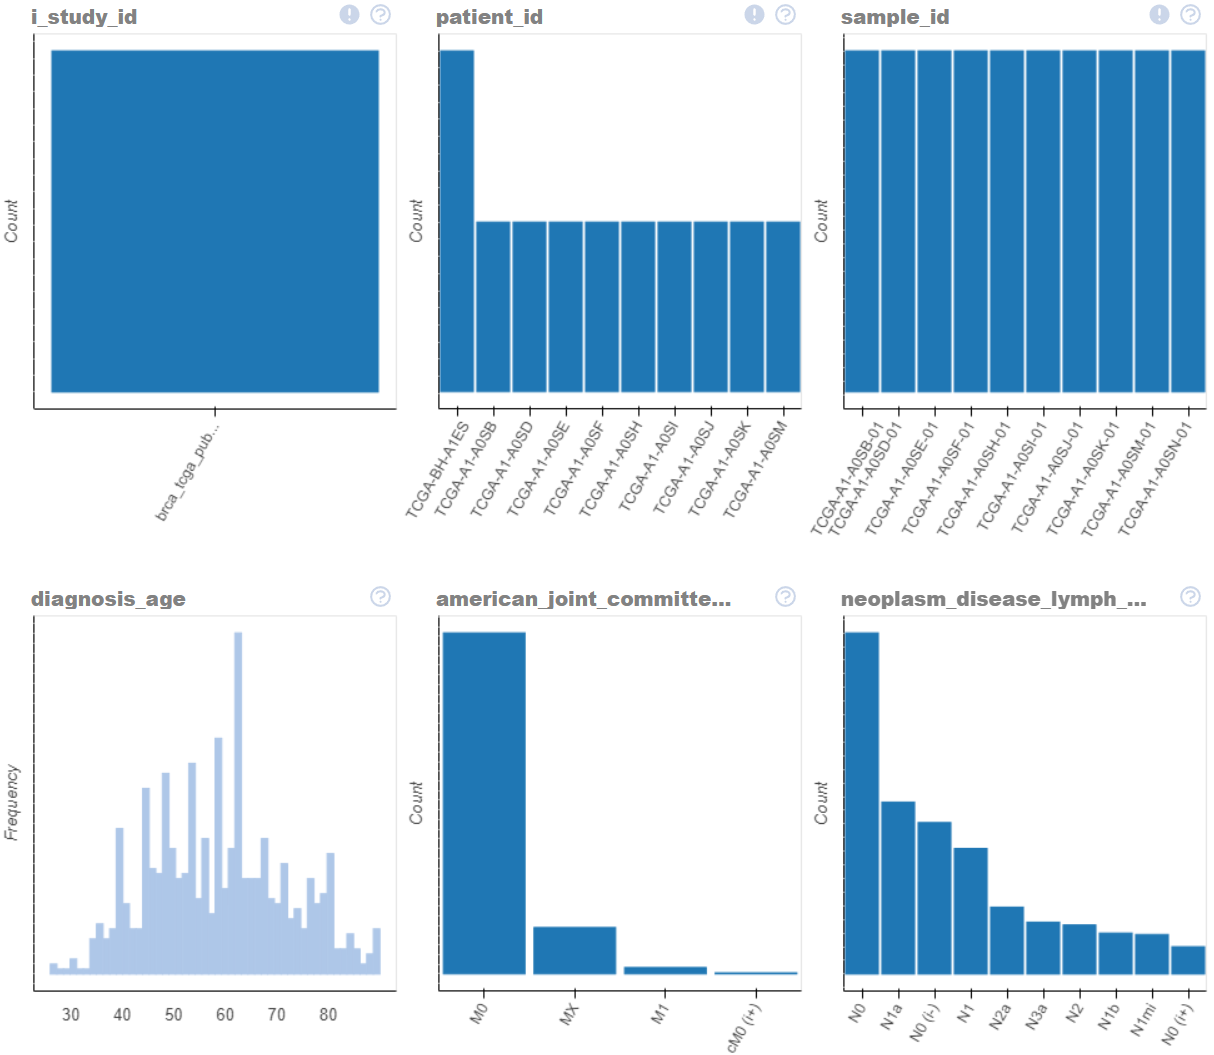
\includegraphics[width=1
	\linewidth]{NOTEBOOK/IMAGES_EDA/1}
\end{figure}

\begin{figure}
	\centering
	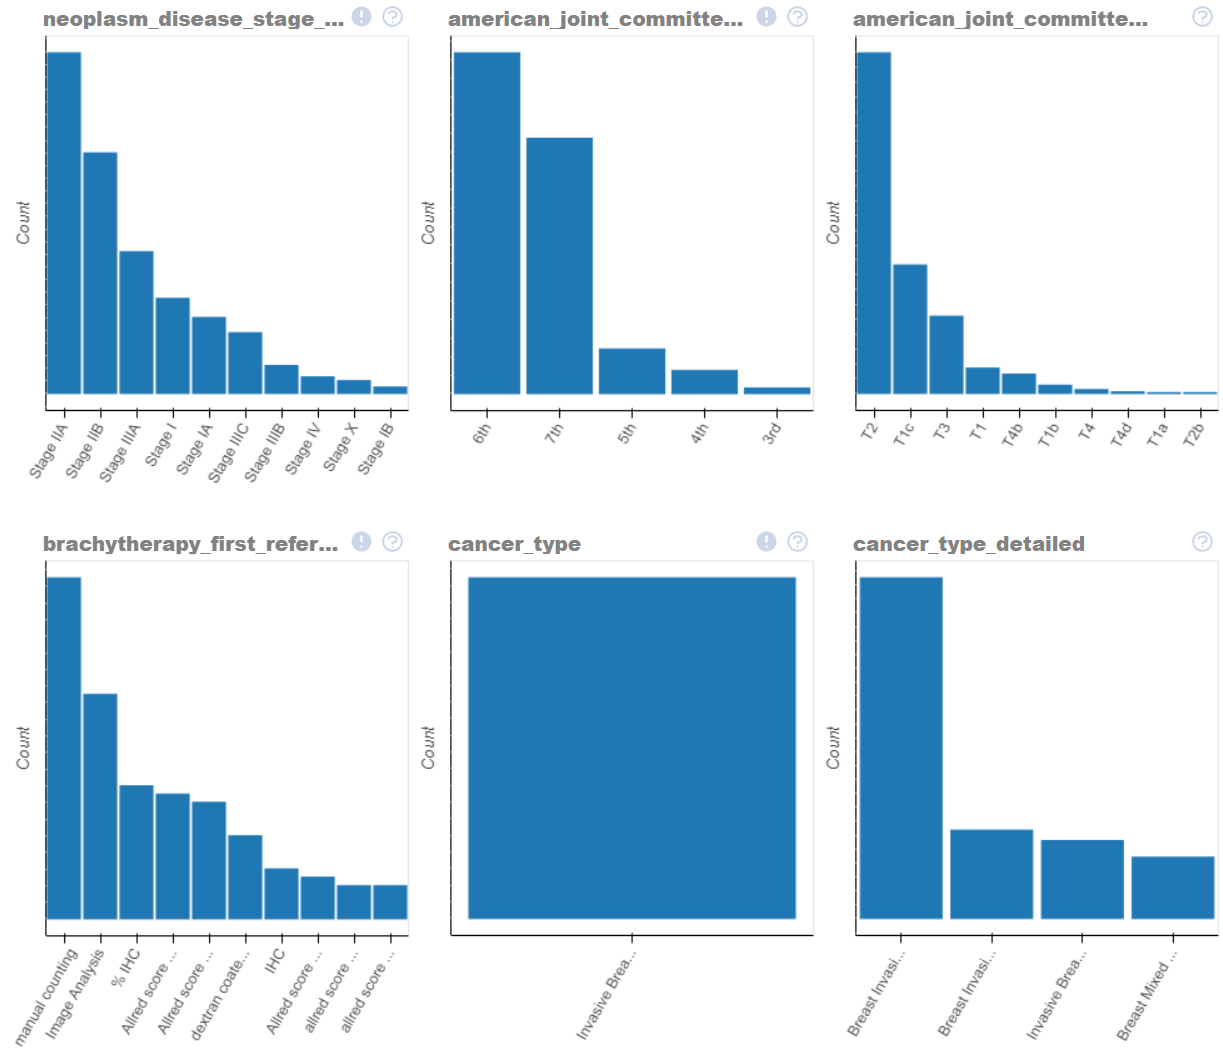
\includegraphics[width=1
	\linewidth]{NOTEBOOK/IMAGES_EDA/2}
\end{figure}

\begin{figure}
	\centering
	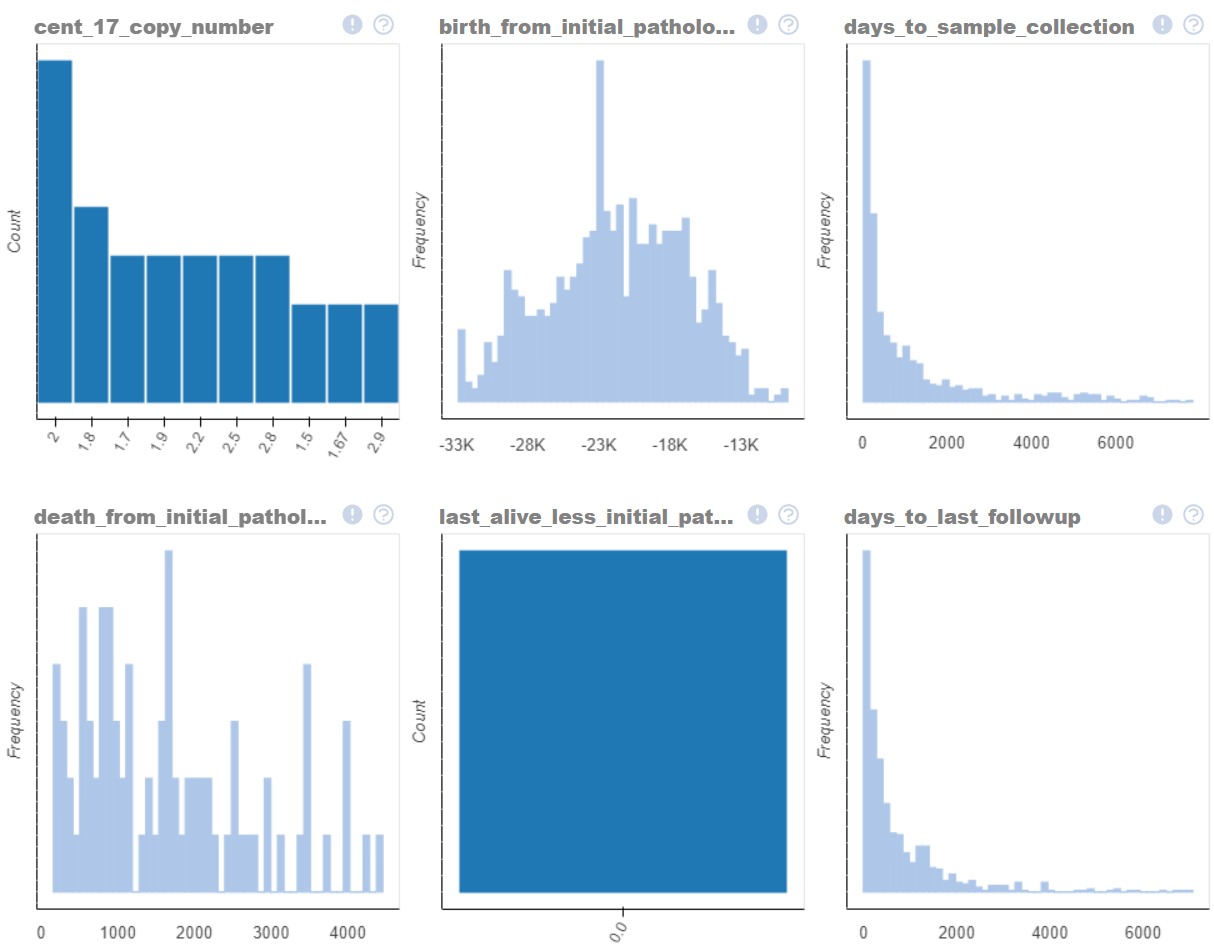
\includegraphics[width=1
	\linewidth]{NOTEBOOK/IMAGES_EDA/3}
\end{figure}

\begin{figure}
	\centering
	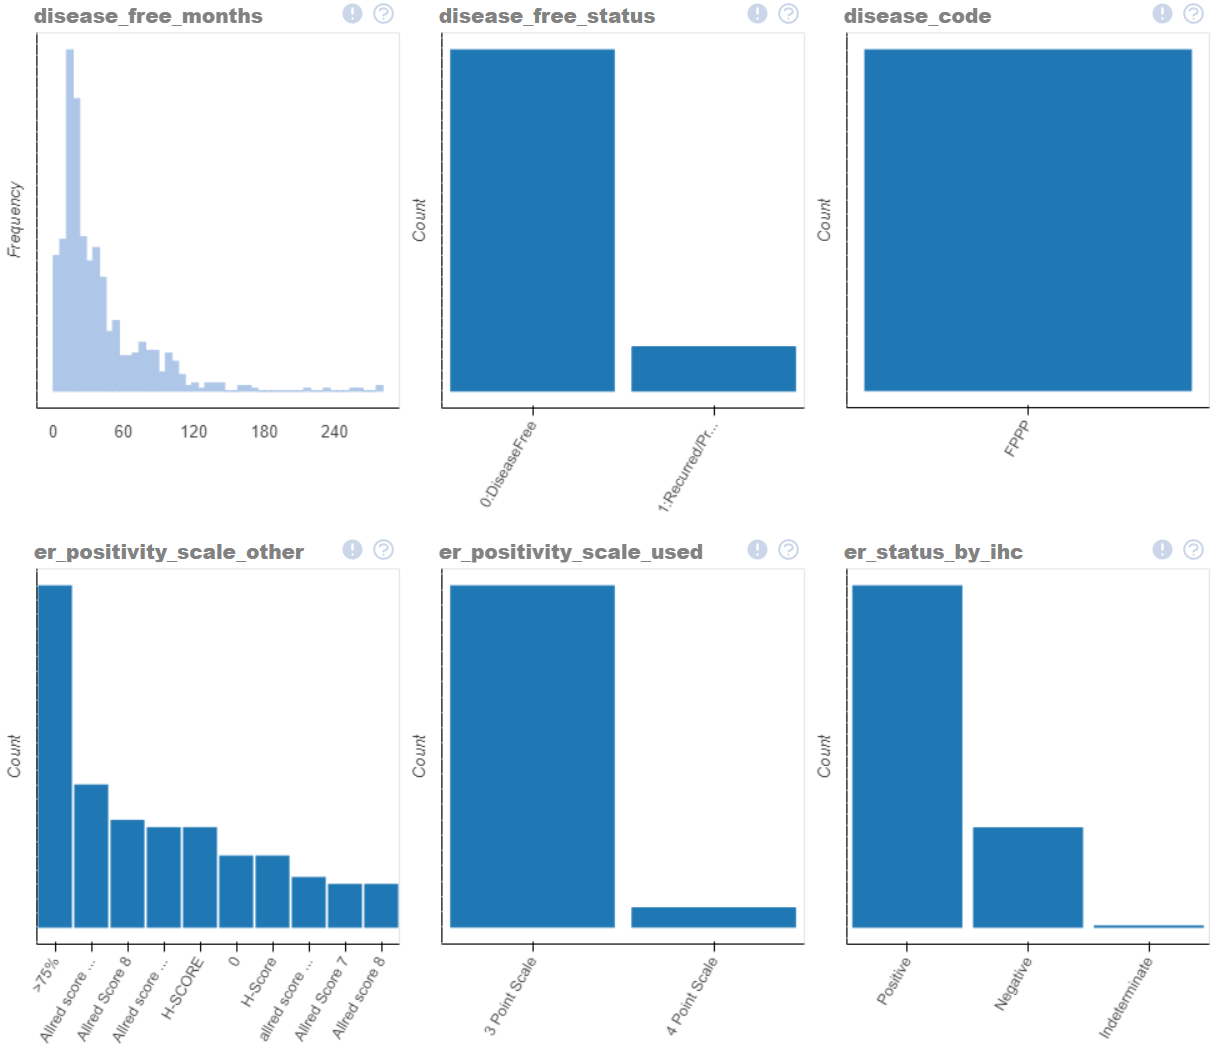
\includegraphics[width=1
	\linewidth]{NOTEBOOK/IMAGES_EDA/4}
\end{figure}

\begin{figure}
	\centering
	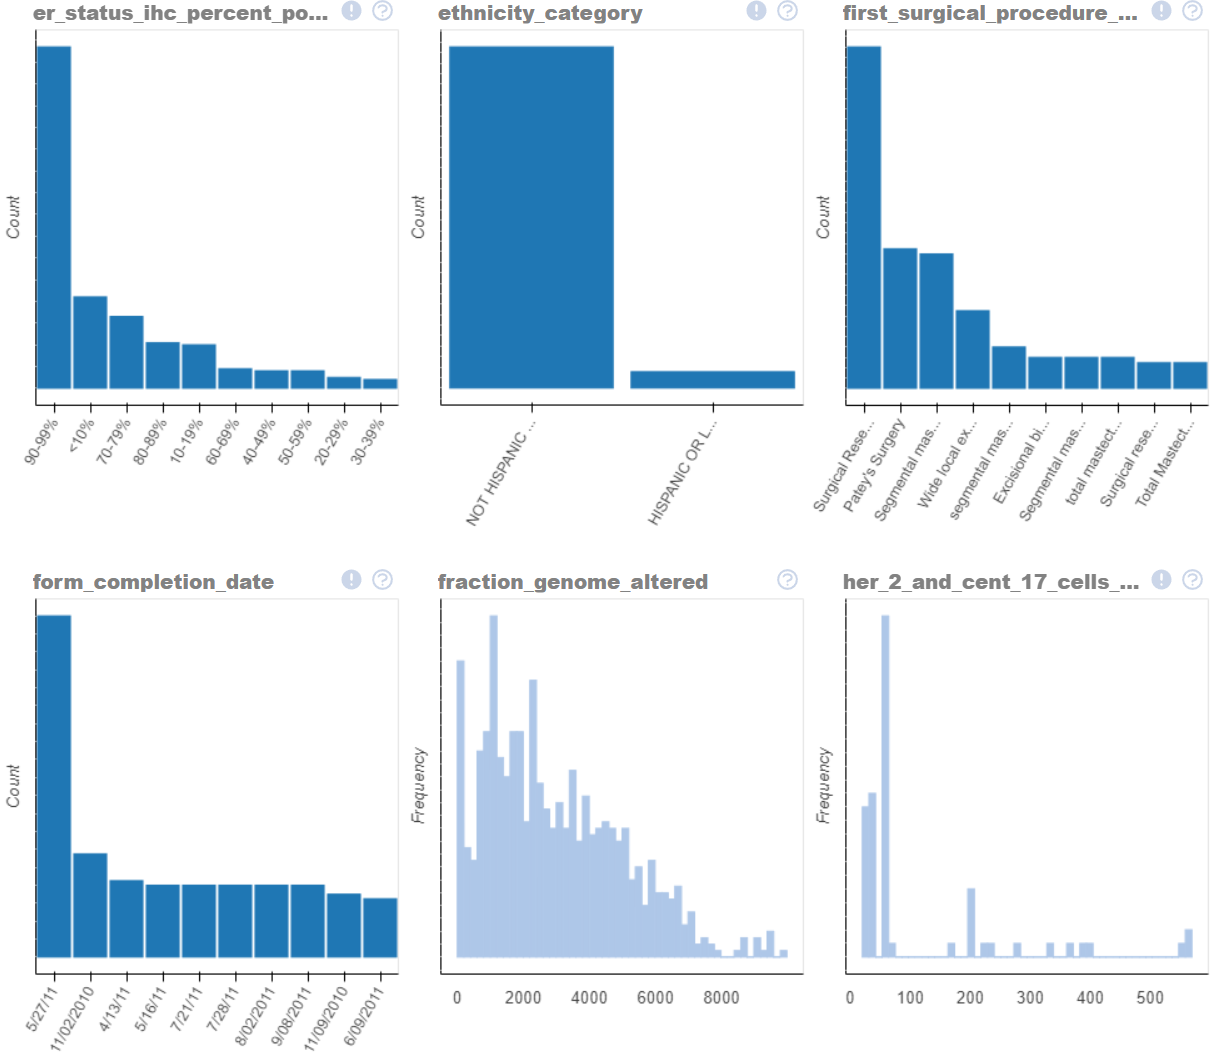
\includegraphics[width=1
	\linewidth]{NOTEBOOK/IMAGES_EDA/5}
	\label{EDA}
	\caption{Distribución del conjunto de datos del Carcinoma invasivo de mama.}\label{fig:foobar}
\end{figure}


\subsection{Detección de datos Ausentes}
En segundo lugar, basados en la obtención de los atributos del conjunto de datos \textit{“Breast Invasive Carcinoma (TCGA, Cell 2015)”}, se realizo un análisis de la cantidad de datos perdidos para identificar las variables y en la etapa posterior realizar la limpieza y el pre-procesamiento de los datos de destino hacerlos consistentes y sin ningún tipo de ruido. Los resultados obtenidos se pueden observar en la figura \ref{Missing_Bar_Chart}:


\begin{figure}[!htb]
	\centering
	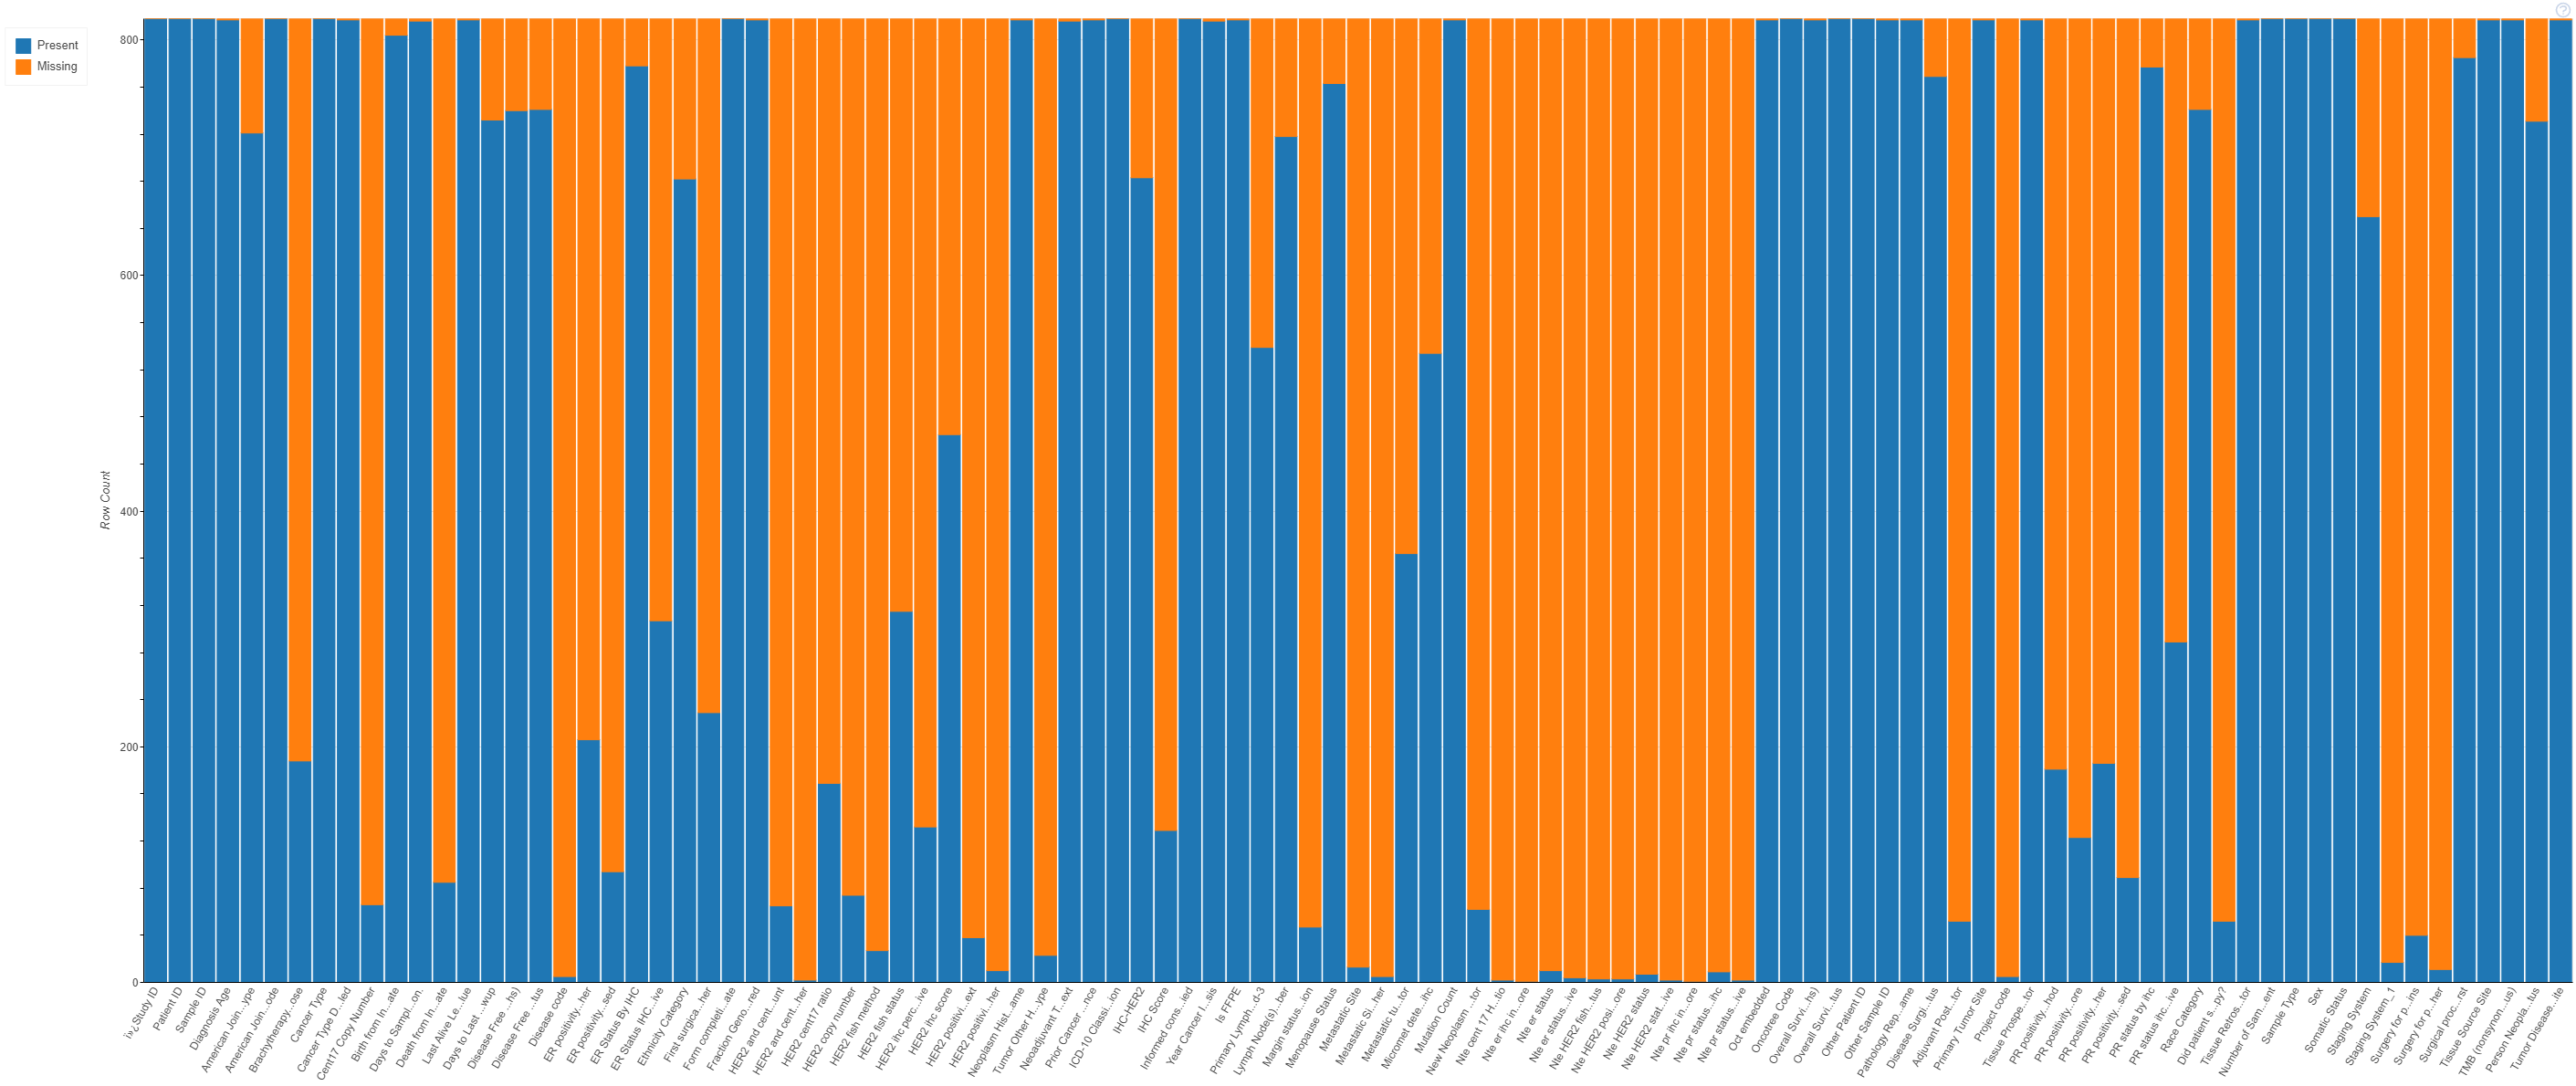
\includegraphics[width=1\linewidth]{IMAGENES/Missing_Bar_Chart}
	\caption{Datos perdidos expresados en una gráfica de barras.}
	\label{Missing_Bar_Chart}
\end{figure}

\begin{figure}[!htb]
	\centering
	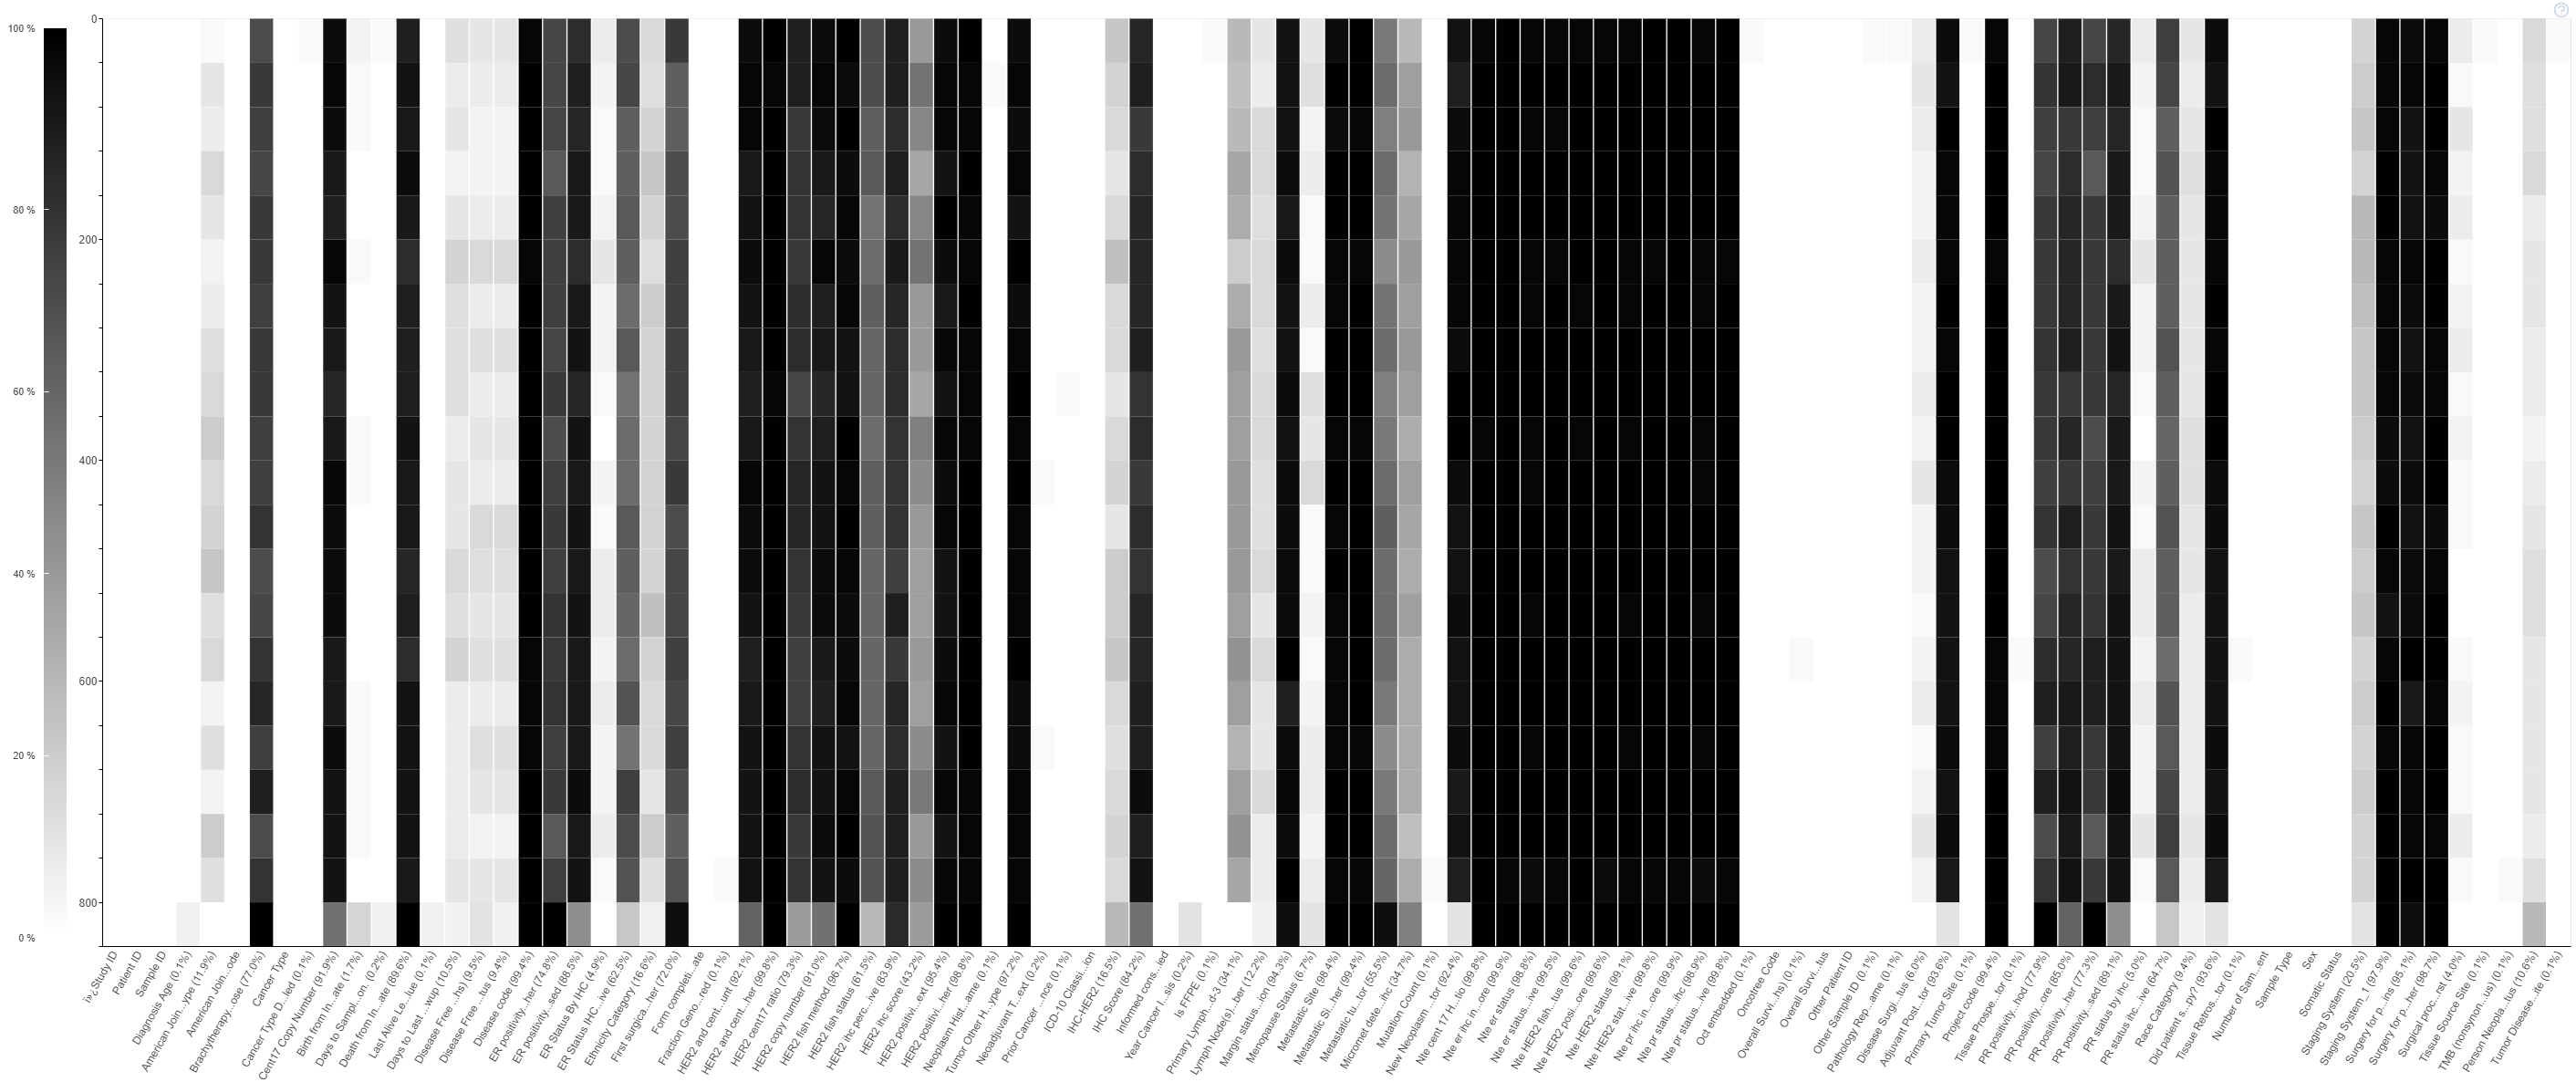
\includegraphics[width=1
	\linewidth]{IMAGENES/Missing_Spectrum}
	\caption{Datos perdidos expresados en un diagrama espectral.}
	\label{Missing_Spectrum}
\end{figure}


\subsection{Análisis Descriptivo }
En primer lugar, se realizo el respectivo análisis descriptivo para detectar cual es comportamiento de los atributos del conjunto de datos \textit{“Breast Invasive Carcinoma (TCGA, Cell 2015)”}. En la gráfica \ref{EDA} se puede observar las gráficas estadísticas unidimensionales de la 110 variables, las cuales permitieron extraer  las características mas representativas y permitieron identificar el comportamiento de los datos.

\begin{table*}[!htb]
	\footnotesize
	\begin{threeparttable}
		\caption{Conjunto de datos del Carcinoma invasivo de mama (TCGA, Cell 2015).}
		\label{Analisis_Descriptivo}
		\begin{tabular}{p{2.5cm} p{7cm} p{6.5cm}} \toprule
			\begin{center}Variable\end{center}   	 
			&\begin{center}Análisis descriptivo\end{center}             
			&\begin{center}Gráfico estadístico\end{center}\\ \hline
			%------------------------------------------------------	
			Diagnosis Age
			& La \textit{edad de diagnostico} del cáncer de mama tiene una tendencia central de 59 años, en donde la edad mínima presentada es de  26 años y la edad máxima presentada es de 90 años.
			
			& \begin{center}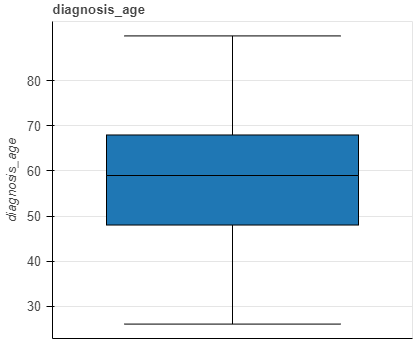
\includegraphics[width=1\linewidth]{NOTEBOOK/IMAGENES_DESCRIPTIVAS/1_diagnosis_age}\end{center}
			\\ \hline
			%------------------------------------------------------	
			AJCC Metastasis Stage Code 
			& El código AJCC para la \textit{estadificación metastásica(M) del cáncer} se visualiza en orden descendente de la siguiente manera: En primer lugar, el código \textit{m0} se presenta en 707 pacientes en donde el cáncer hizo metástasis pero no se  disemino a otras partes del cuerpo. En segundo lugar se encuentra el código \textit{mx} presentado en 96 pacientes a los cuales no fue posible medir la metástasis. En tercer lugar se encuentra el código \textit{m1} presentado en 13 pacientes en donde el cáncer se diseminó a otras partes del cuerpo. En ultimo lugar se encuentra el código \textit{cM0(i+)} presentado en 2 pacientes en los cuales no se detecto evidencia de metástasis a distancia, pero hubo un pequeño número de células en las cuales se encontró una metástasis diminuta (no mayor de 0.2 mm) detectada en ganglios linfáticos no regionales \cite{NCI}.
			
			& \begin{center}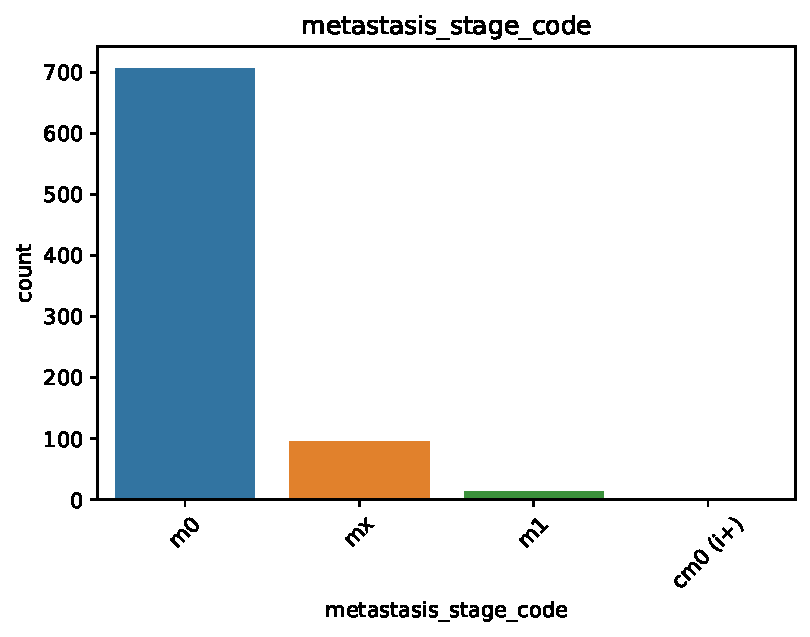
\includegraphics[width=1\linewidth]{NOTEBOOK/IMAGENES_DESCRIPTIVAS/2_metastasis_stage_code}\end{center}
			\\ \hline
			%------------------------------------------------------	
			AJCC Neoplasm Disease Lymph Node Stage Code
			& El código AJCC para la \textit{estadificación del cáncer por neoplasia del ganglio linfático(N)} se visualiza en orden descendente de la siguiente manera: En primer lugar, el código \textit{n0} se presenta en 250 pacientes en donde no hay cáncer en los ganglios linfáticos cercanos. En segundo lugar, el código \textit{n1a} se presento en 126 pacientes en donde el cáncer se diseminó a 1 ganglio linfáticos debajo del brazo con al menos un área de cáncer diseminada de más de 2 mm de ancho. En tercer lugar el código \textit{n0(i-)} se presento en 126 pacientes en donde, no hay evidencia histológica de metástasis en los ganglios linfáticos regionales. Del cuarto lugar en adelante, se refiere a la cantidad y ubicación de los ganglios linfáticos que contienen cáncer. Cuanto mayor sea el número después de la $n$, más ganglios linfáticos se vieron afectados.	
			
			& \begin{center}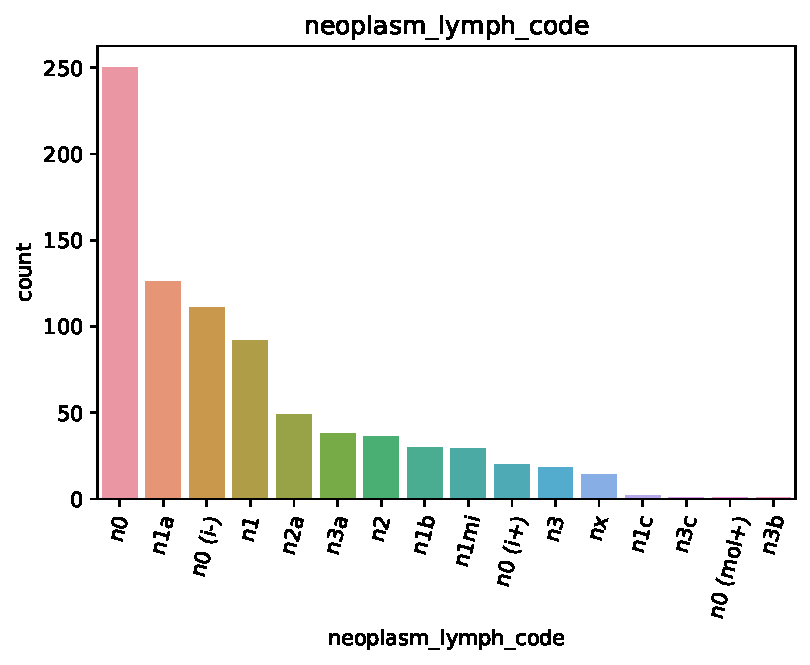
\includegraphics[width=1\linewidth]{NOTEBOOK/IMAGENES_DESCRIPTIVAS/3_neoplasm_lymph_code}\end{center}
			\\ \hline
			%------------------------------------------------------	
		\end{tabular}
	\end{threeparttable}
\end{table*}

\begin{table*}[!htb]
	\footnotesize
	\begin{threeparttable}
		\begin{tabular}{p{2.5cm} p{7cm} p{6.5cm}} \toprule
			%------------------------------------------------------	
			AJCC Neoplasm Disease Stage Code
			& Las etapas AJCC para la \textit{estadificación del cáncer por neoplasia} se visualiza en orden descendente de la siguiente manera: En primer lugar, la \textit{etapa iia} se presenta en 278 pacientes en donde el tumor mide más de 20 mm pero no más de 50 mm y no se ha propagado a los ganglios linfáticos axilares. En segundo lugar, la \textit{etapa iib} se presento en 190 pacientes en donde el tumor mide más de 50 mm pero no se ha propagado a los ganglios linfáticos axilares. En tercer lugar la \textit{etapa iiia} se presento en 112 pacientes en donde el tumor se diseminó de 4 a 9 ganglios linfáticos axilares o los ganglios linfáticos mamarios internos, pero no se ha propagado a otras partes del cuerpo. En cuarto lugar, la \textit{etapa i} se presento en 75 pacientes  en donde el tumor es pequeño, invasivo y no se ha propagado a los ganglios linfáticos. En quinto lugar, la \textit{etapa ia} se presento en 60 pacientes en donde el tumor mide menos de 20 mm  y no se ha propagado a los ganglios linfáticos. Del sexto lugar en adelante, el tumor puede tener cualquier tamaño y se ha propagado a otros órganos, como los huesos, los pulmones, el cerebro, el hígado, los ganglios linfáticos distantes o la pared torácica.
			
			& \begin{center}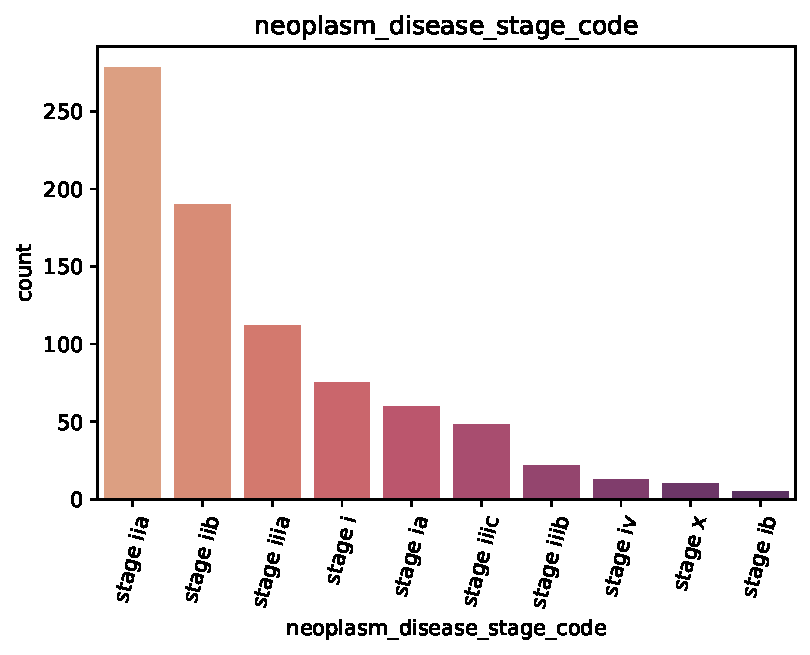
\includegraphics[width=1\linewidth]{NOTEBOOK/IMAGENES_DESCRIPTIVAS/4_neoplasm_disease_stage_code}\end{center}
			\\ \hline
			%------------------------------------------------------	
			AJCC Tumor Stage Code 
			& El código AJCC para la \textit{estadificación el tumor (T) primario del cáncer} se visualiza en orden descendente de la siguiente manera: En primer lugar, el código \textit{t2} se presenta en 459 pacientes en donde el tumor mide más de 20 mm pero no más de 50 mm. En segundo lugar, el código \textit{t1c} se presento en 173 pacientes en donde el tumor mide  de 10 mm a 20 mm o menos. En tercer lugar el código \textit{t3} se presento en 104 pacientes en donde el tumor mide más de 50 mm. En cuarto lugar el código \textit{t1} se presento en 34 pacientes en donde el tumor  mide 20 mm o menos en su área más ancha. En quinto lugar el código \textit{t4b} se presento en 26 pacientes en donde el tumor ha crecido dentro de la piel. Del sexto lugar en adelante, el código \textit{t1b} se presento en 11 pacientes en donde el tumor mide más de 5 mm pero menos de 10 mm, el código \textit{t4} se presento en 5 pacientes en donde el tumor ha crecido hacia la pared torácica, el código \textit{t4d} se presento en 2 pacientes en donde es cáncer de mama inflamatorio, el código \textit{t1a} se presento en 1 paciente en donde el tumor mide más de 1 mm pero menos de 5 mm, el código \textit{t2b} se presento en 1 paciente en donde el tumor mide más de el tumor mide más de 25 mm pero menos de 50 mm.
			
			& \begin{center}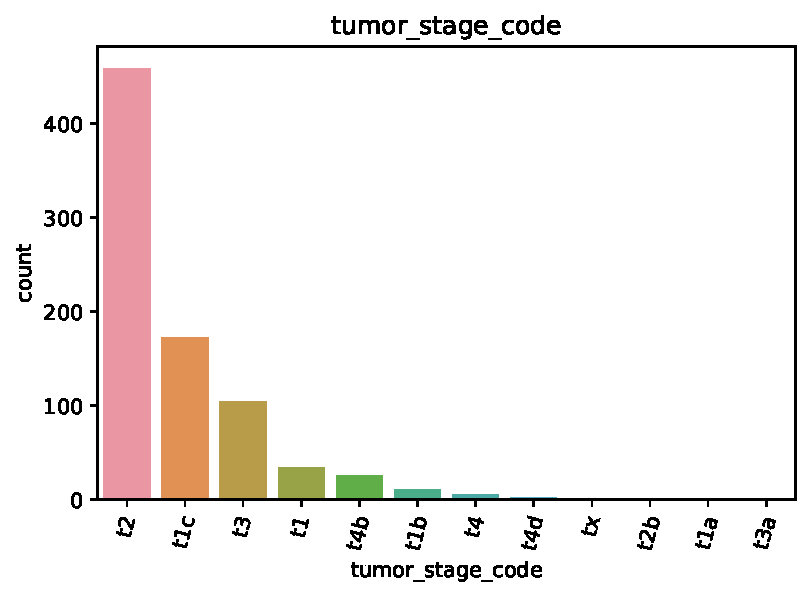
\includegraphics[width=1\linewidth]{NOTEBOOK/IMAGENES_DESCRIPTIVAS/5_tumor_stage_code}\end{center}
			\\ \hline
		\end{tabular}
	\end{threeparttable}
\end{table*}


\begin{table*}[!htb]
	\footnotesize
	\begin{threeparttable}
		\begin{tabular}{p{2.5cm} p{7cm} p{6.5cm}} \toprule
			%------------------------------------------------------	
			Cancer Type Detailed
			& El \textit{tipo de cáncer de mama} se visualiza en orden descendente de la siguiente manera: En primer lugar, el \textit{cáncer Ductal invasivo} se presento en 491 pacientes. En segundo  lugar, el \textit{cáncer Lobulillar invasivo} se presento en 127 pacientes. En tercer lugar, el \textit{cáncer invasivo con otros diagnósticos} se presento en 112 pacientes. En cuarto lugar,  el \textit{cáncer mixto (Ductal y Lobulillar)} se presento en 88 pacientes.
			
			& \begin{center}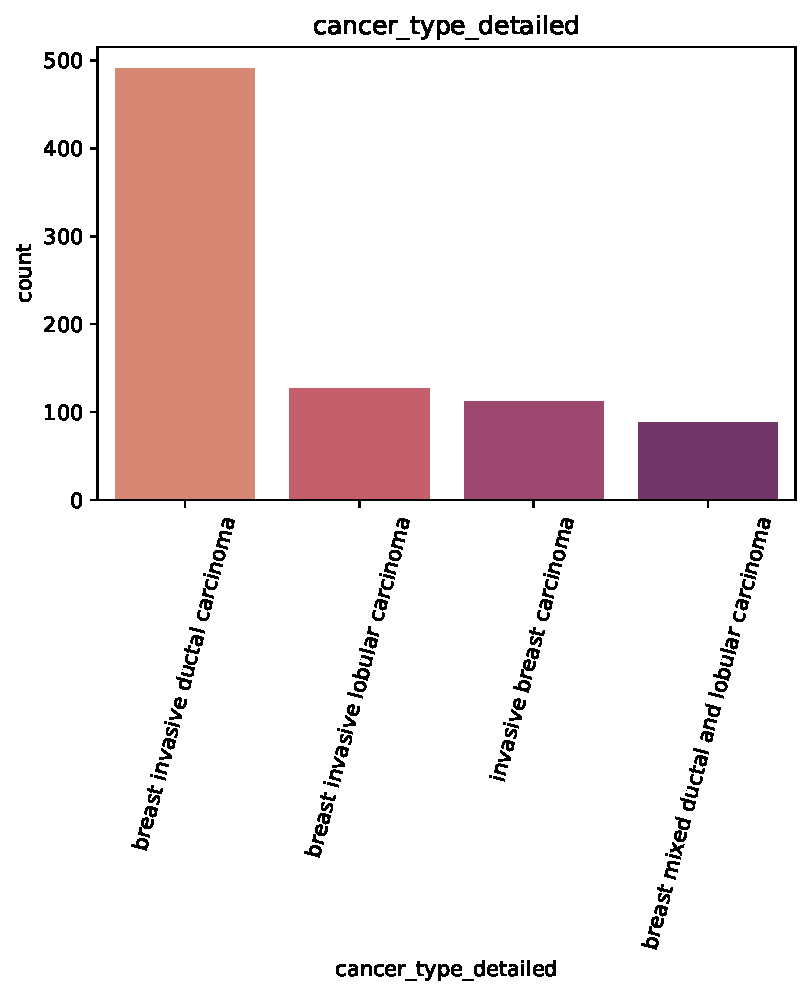
\includegraphics[width=1\linewidth]{NOTEBOOK/IMAGENES_DESCRIPTIVAS/6_cancer_type_detailed}\end{center}
			\\ \hline
			%------------------------------------------------------	
			Days to Sample Collection
			& El intervalo de días para la \textit{recolección de muestras} tiene una tendencia central aproximada de 451 días, en donde el tiempo mínimo presentado es de 16 días y el tiempo máximo presentado de 7804 días.
			
			& \begin{center}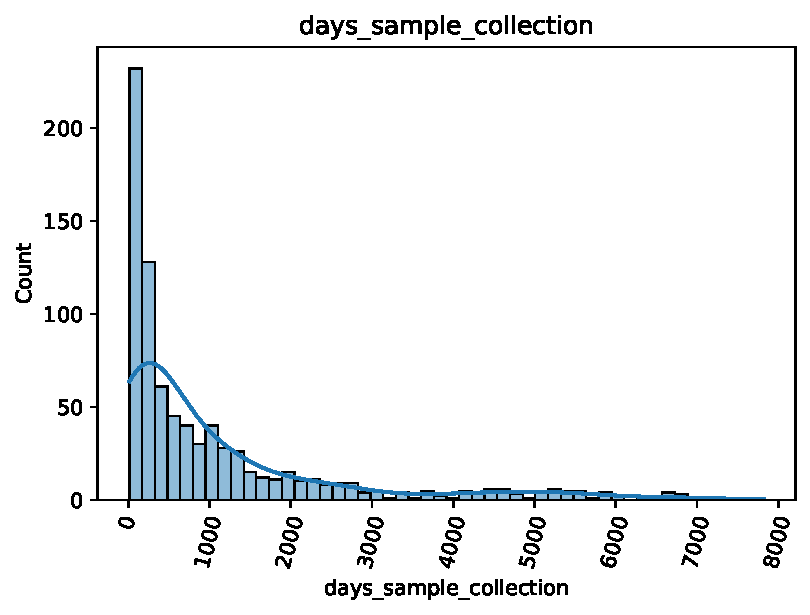
\includegraphics[width=1\linewidth]{NOTEBOOK/IMAGENES_DESCRIPTIVAS/7_days_sample_collection}\end{center}
			\\ \hline
			%------------------------------------------------------	
			Days to Last Followup
			& El Intervalo de tiempo desde la fecha del \textit{último seguimiento} hasta la fecha del diagnóstico patológico inicial tiene una tendencia central aproximada de 579 días, en donde el tiempo mínimo de diagnostico  presentado es de 1 día y el tiempo maximo de diagnostico presentado de 7067 días.
			
			& \begin{center}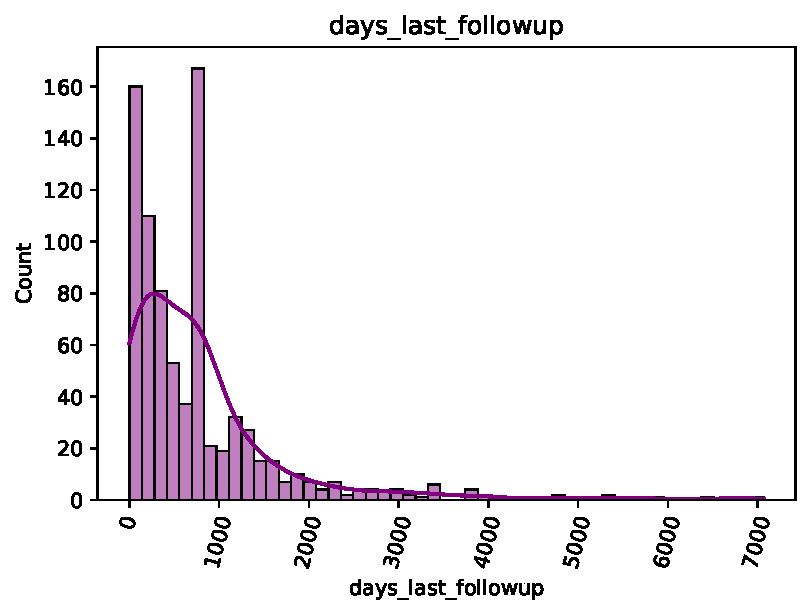
\includegraphics[width=1\linewidth]{NOTEBOOK/IMAGENES_DESCRIPTIVAS/8_days_last_followup}\end{center}
			\\ \hline
		\end{tabular}
	\end{threeparttable}
\end{table*}


\begin{table*}[!htb]
	\footnotesize
	\begin{threeparttable}
		\begin{tabular}{p{2.5cm} p{7cm} p{6.5cm}} \toprule
			%------------------------------------------------------	
			Disease Free (Months)
			& El Intervalo de \textit{meses sin enfermedad} tiene una tendencia central aproximada de 32 meses, en donde el tiempo mínimo presentado es de 16 meses y el tiempo máximo presentado de 281 meses.
			
			& \begin{center}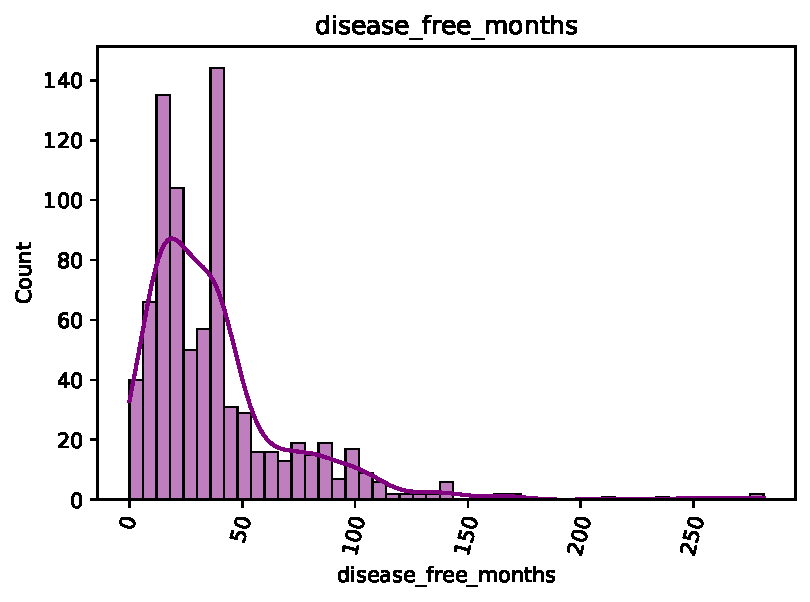
\includegraphics[width=1\linewidth]{NOTEBOOK/IMAGENES_DESCRIPTIVAS/9_disease_free_months}\end{center}
			\\ \hline
			
			%------------------------------------------------------	
			Disease Free Status
			& El \textit{estado libre de enfermedad} se clasifica de forma nominal en dos categorías: La primera categoría corresponde al estado \textit{disease free} en donde se encuentran 733 pacientes que estuvieron libre de enfermedad durante un tiempo determinado y la segunda categoría corresponde al estado el estado \textit{progressed} en donde se encuentran 85 pacientes en donde la enfermedad fue avanzando de manera progresiva. 
			
			& \begin{center}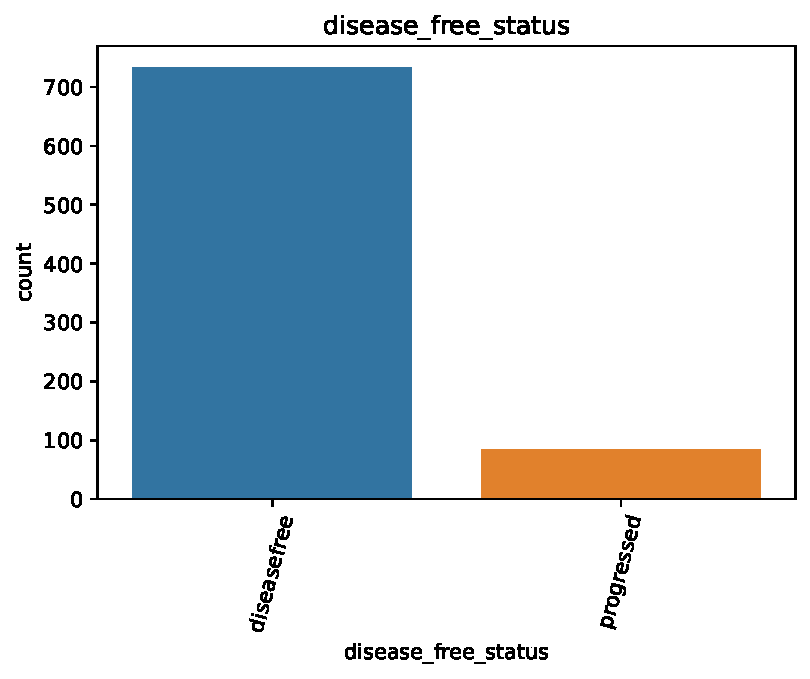
\includegraphics[width=1\linewidth]{NOTEBOOK/IMAGENES_DESCRIPTIVAS/10_disease_free_status}\end{center}
			\\ \hline
			
			%------------------------------------------------------	
			ER positivity scale other
			&La variable \textit{Otra escala de receptor de estrogeno positivo} se visualiza en orden descendente de la siguiente manera: En primer lugar, la escala \textit{allred score 8} se presenta en 671 pacientes que tienen células cancerosas con receptores positivos de estrogeno con un crecimiento fuerte. En segundo lugar, la escala $>$\textit{75\%} se presento en 48 pacientes que tienen células cancerosas con receptores positivos de estrogeno con un crecimiento anormal. En tercer lugar la escala \textit{h-score} se presento en 26 pacientes con un porcentaje moderado de células tumorales con tinción de membrana celular positivo de estrogeno. En cuarto, la escala \textit{allred score 0} se presenta en 15 pacientes que tienen células cancerosas con receptores negativos de estrogeno. Del quinto lugar en adelante, los pacientes presentan células cancerosas con receptores positivos de estrogeno con un comportamiento de crecimiento moderado.
			& \begin{center}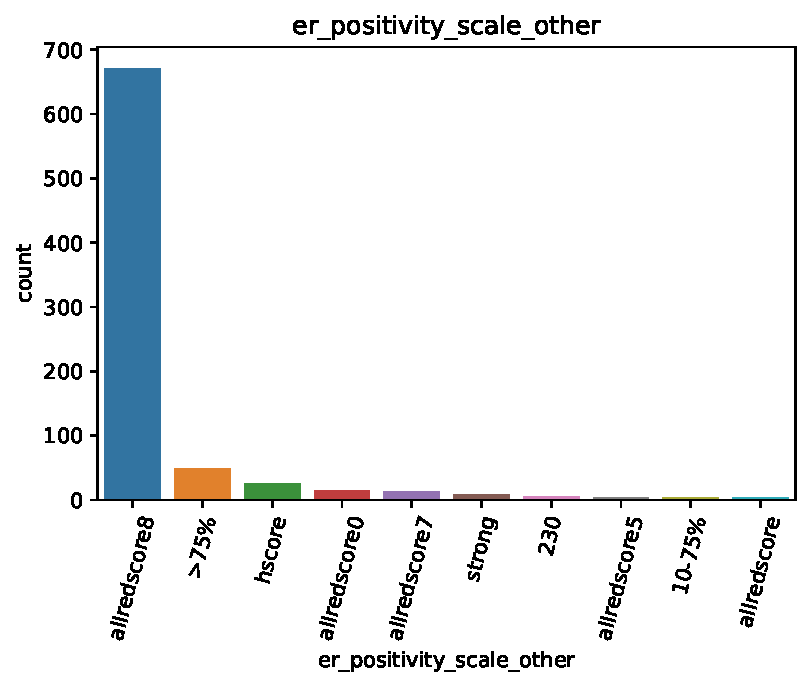
\includegraphics[width=1\linewidth]{NOTEBOOK/IMAGENES_DESCRIPTIVAS/11_er_positivity_scale_other}\end{center}
			\\ \hline
		\end{tabular}
	\end{threeparttable}
\end{table*}

\begin{table*}[!htb]
	\footnotesize
	\begin{threeparttable}
		\begin{tabular}{p{2.5cm} p{7cm} p{6.5cm}} \toprule
			ER Status By IHC
			&El \textit{Estado del receptor de estrogeno por análisis IHC} se clasifica de forma nominal en dos categorías: La primera categoría corresponde al estado \textit{positive} en donde se encuentran 643 pacientes a los cuales al realizar el análisis de inmunohistoquímica(IHC) sobre tejido mamario canceroso se determino que las células cancerosas tienen receptores positivos de estrogeno y la segunda categoría corresponde al estado \textit{negative} en donde se encuentran 175 pacientes a los cuales al realizar el análisis IHC sobre tejido mamario canceroso se determino que las células cancerosas no presentan receptores de estrogeno.
			& \begin{center}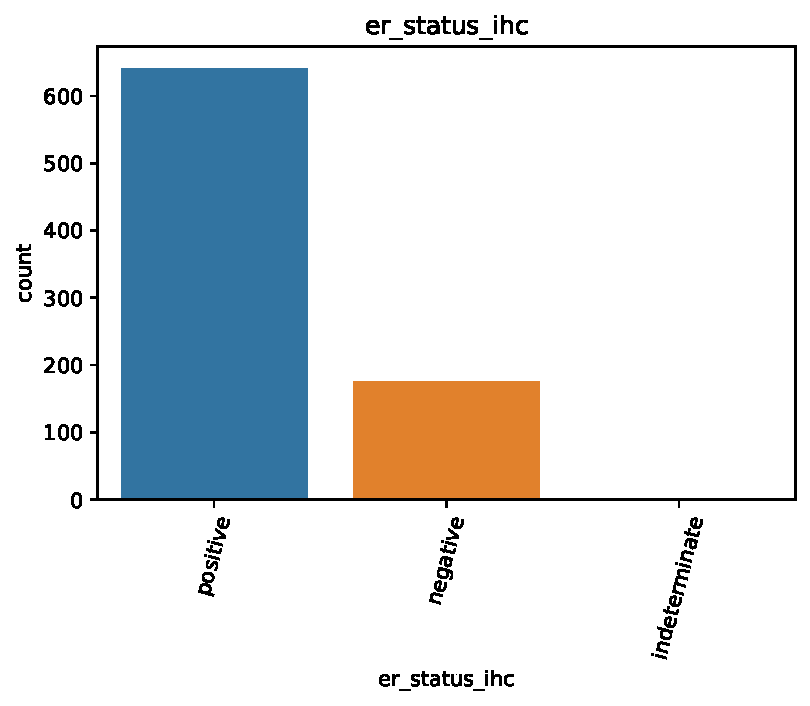
\includegraphics[width=1\linewidth]{NOTEBOOK/IMAGENES_DESCRIPTIVAS/13_er_status_ihc}\end{center}
			\\ \hline
			
			%------------------------------------------------------	
			ER Status IHC Percent Positive
			&El \textit{Estado del porcentaje del receptor de estrogeno por análisis IHC} se visualiza en orden descendente de la siguiente manera: En primer lugar, 668 pacientes presentan células cancerosas con receptores positivos de estrogeno en un \textit{90-99\%} obre tejido mamario. En segundo lugar, 42 pacientes presentan células cancerosas con receptores positivos de estrogeno en un $<$\textit{10\%} sobre tejido mamario. En tercer lugar, 33 pacientes presentan células cancerosas con receptores positivos de estrogeno en un \textit{70-79\%} sobre tejido mamario. En cuarto lugar, 21 pacientes presentan células cancerosas con receptores positivos de estrogeno en un \textit{80-89\%} sobre tejido mamario. En quinto lugar, 20 pacientes presentan células cancerosas con receptores positivos de estrogeno en un \textit{10-19\%} sobre tejido mamario. Del sexto lugar en adelante, los pacientes presentan células cancerosas con receptores positivos de estrogeno con un porcentaje variable.
			& \begin{center}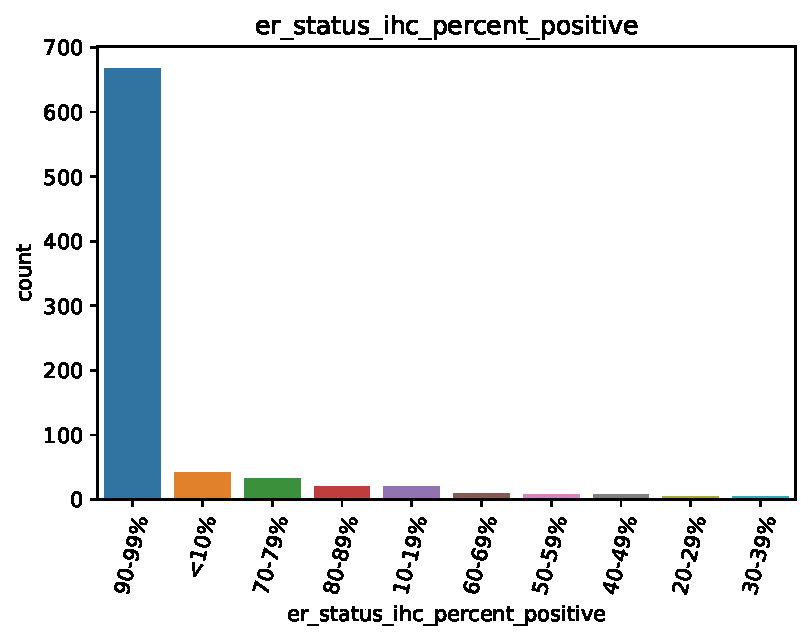
\includegraphics[width=1\linewidth]{NOTEBOOK/IMAGENES_DESCRIPTIVAS/14_er_status_ihc_percent_positive}\end{center}
			\\ \hline
			
			%------------------------------------------------------	
			Ethnicity Category
			&La \textit{Categoría étnica} se clasifica de forma nominal en dos categorías: La primera categoría corresponde al estado \textit{not hispanic or latino} en donde se encuentran 787 pacientes que no presentan una ascendencia latina o de origen español y la segunda categoría corresponde al estado estado \textit{hispanic or latino} en donde se encuentran 31 pacientes que presentan una ascendencia latina o de origen español.
			& \begin{center}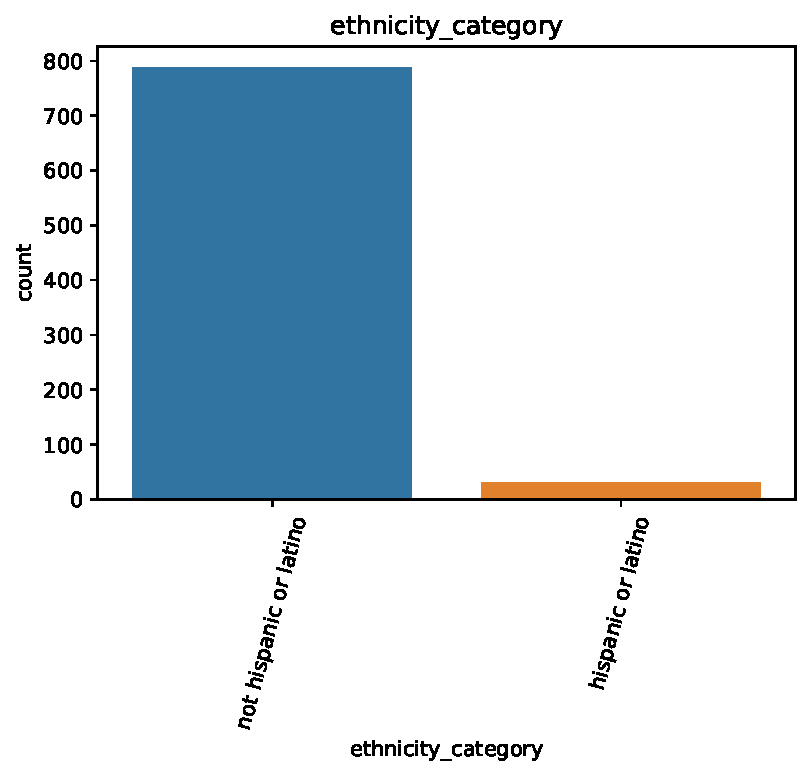
\includegraphics[width=1\linewidth]{NOTEBOOK/IMAGENES_DESCRIPTIVAS/15_ethnicity_category}\end{center}
			\\ \hline
			
		\end{tabular}
	\end{threeparttable}
\end{table*}

\begin{table*}[!htb]
	\footnotesize
	\begin{threeparttable}
		\begin{tabular}{p{2.5cm} p{7cm} p{6.5cm}} \toprule
			%------------------------------------------------------	
			First surgical procedure other
			& La \textit{Primera intervención quirúrgica} se visualiza en orden descendente de la siguiente manera: En primer lugar, la intervención quirúrgica \textit{surgical resection} se realizo a 660 pacientes a los cuales se les extirpo todo el tumor o la mayor cantidad posible del mismo. 	En segundo lugar, la intervención quirúrgica \textit{pateys surgery} se realizo a 44 pacientes a los cuales se les extirpo todo el seno, incluida la piel, el tejido mamario, la areola y el pezón junto con la mayoría de los ganglios linfáticos axilares. En tercer lugar, la intervención quirúrgica \textit{surgical resection} se realizo a 34 pacientes a los cuales se les extirpo el cáncer u otro tejido anormal del seno y parte del tejido normal que lo rodea, pero no el seno en sí. En cuarto lugar, la intervención quirúrgica \textit{wide local excision} se realizo a 17 pacientes a los cuales se uso un bisturí para extirpar un tumor u otra lesión anormal y parte del tejido normal que lo rodeaba. En quinto lugar, la intervención quirúrgica \textit{exicional biposy} se realizo a 8 pacientes a los cuales se les extirpo una masa completa o área sospechosa. Del sexto lugar en adelante se utilizaron otros tipos de intervenciones quirúrgicas.
			
			& \begin{center}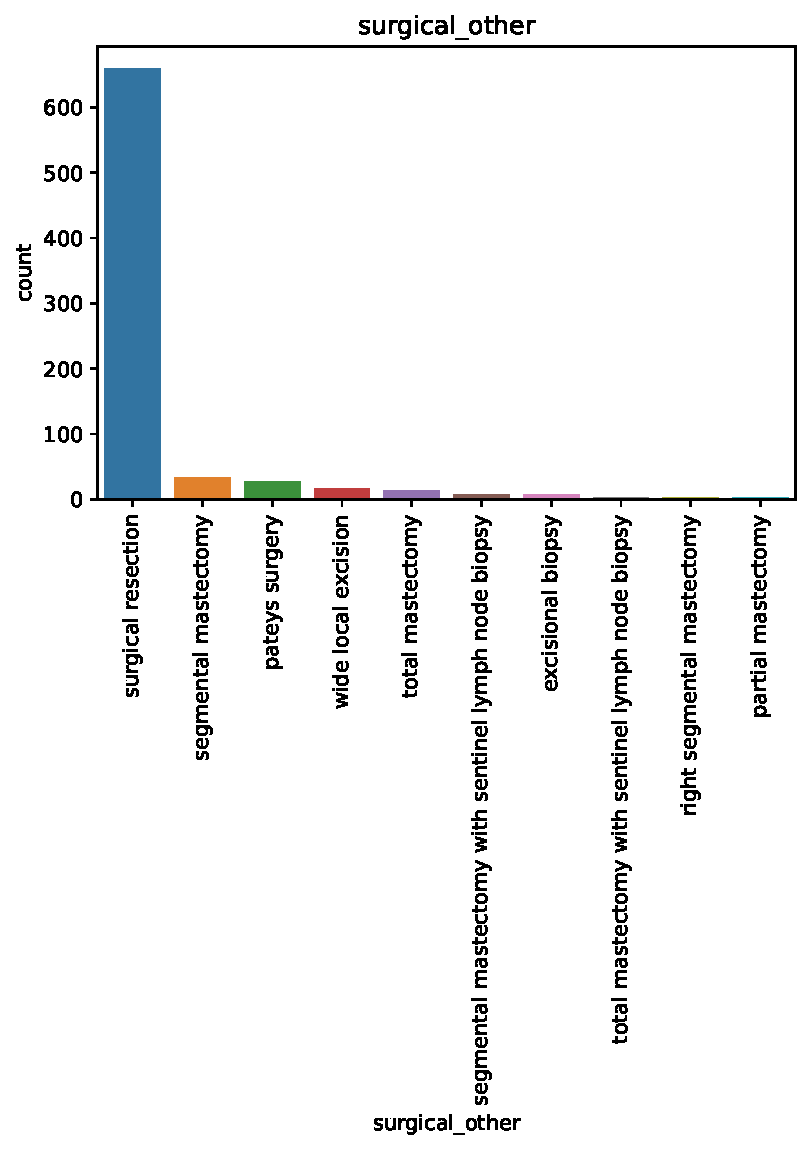
\includegraphics[width=1\linewidth]{NOTEBOOK/IMAGENES_DESCRIPTIVAS/16_surgical_other}\end{center}
			\\ \hline
			
			%------------------------------------------------------	
			Fraction Genome Altered
			& La \textit{Estabilidad genómica} o también llamado \textit{Fenotipo mutador} necesaria para que las células acumulen múltiples mutaciones estimulando el desarrollo del cáncer, presenta un tendencia central de 25.07\% relacionado a genes que se han visto afectados por las ganancias o pérdidas del número de copias celulares, en donde el porcentaje mínimo presentado es del 12,22\% y el máximo del 99,71\%
			
			& \begin{center}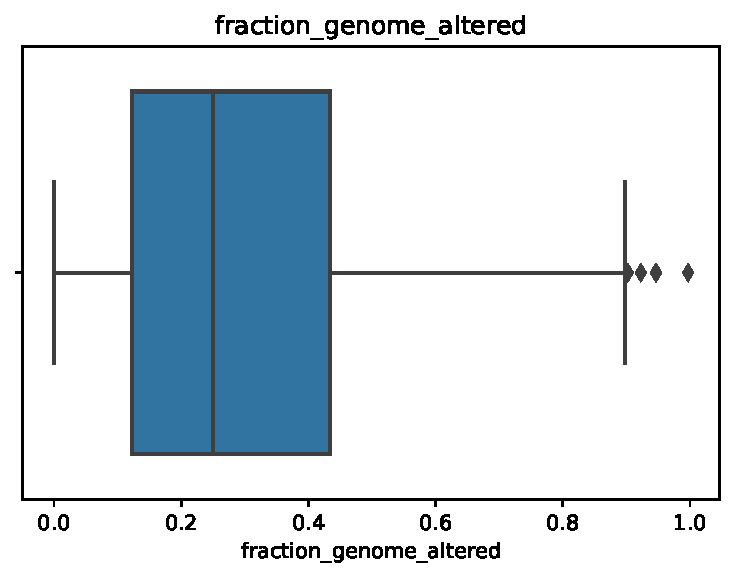
\includegraphics[width=1\linewidth]{NOTEBOOK/IMAGENES_DESCRIPTIVAS/17_fraction_genome_altered}\end{center}
			\\ \hline
			
			%------------------------------------------------------	
			HER2 fish status
			& La \textit{prueba FISH (hibridación fluorescente in situ)} analiza el ADN de las células cancerosas en busca de copias adicionales del gen \textit{HER2 (Receptor 2 del factor de crecimiento epidérmico humano)}. En este caso el \textit{estado FISH} se clasifica de forma nominal en dos categorías: La primera categoría corresponde al estado \textit{negativo} en donde se encuentran 758 pacientes en los cuales la proteína HER2 no está involucrada en el crecimiento del tumor mamario y la segunda categoría corresponde al estado \textit{Positivo} en donde se encuentran 60 pacientes en los cuales las células cancerígenas producen demasiada HER2 estimulando el crecimiento del tumor mamario. 
			& \begin{center}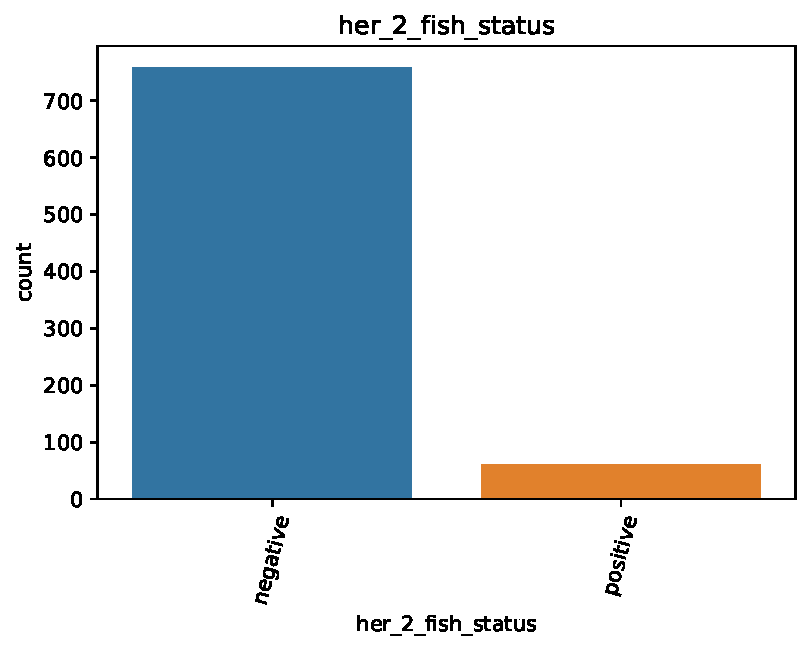
\includegraphics[width=1\linewidth]{NOTEBOOK/IMAGENES_DESCRIPTIVAS/19_her_2_fish_status}\end{center}
			\\ \hline
		\end{tabular}
	\end{threeparttable}
\end{table*}

\begin{table*}[!htb]
	\footnotesize
	\begin{threeparttable}
		\begin{tabular}{p{2.5cm} p{7cm} p{6.5cm}} \toprule
			%------------------------------------------------------	
			HER2 ihc percent positive
			& El \textit{Porcentaje positivo de HER2 según la prueba de inmunohistoquímica (IHC)}, se visualiza en orden descendente de la siguiente manera: En primer lugar, 757 pacientes presentan tinción apenas perceptible, observada en un valor $<$\textit{10\%} de las células tumorales. En segundo lugar, 17 pacientes presentan una tinción de membrana moderada observada en \textit{10-19\%} de las células tumorales. En tercer lugar, 12 pacientes presentan una tinción de membrana intensa observada en \textit{90-99\%} de las células tumorales. Del cuarto lugar en adelante, los pacientes presentan una tinción de membrana variable en un rango de débil a moderada.
			& \begin{center}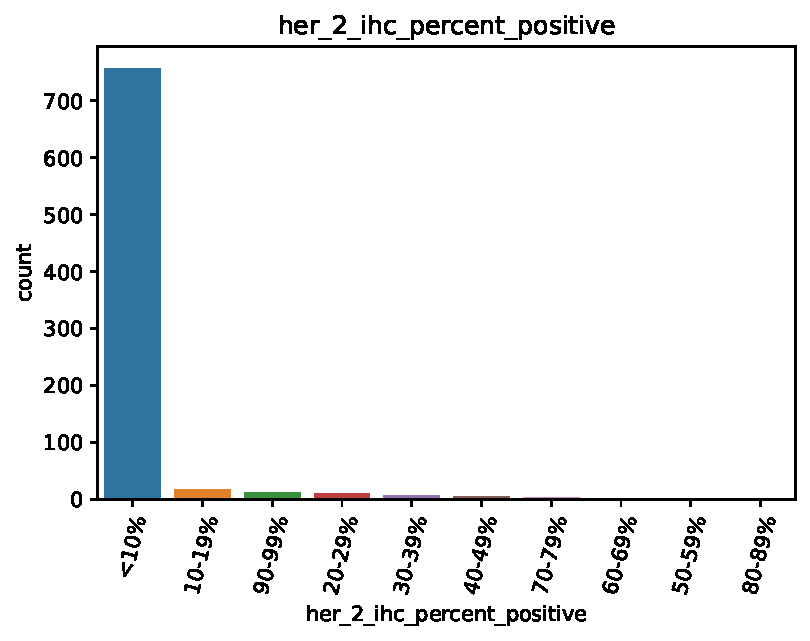
\includegraphics[width=1\linewidth]{NOTEBOOK/IMAGENES_DESCRIPTIVAS/20_her_2_ihc_percent_positive}\end{center}
			\\ \hline
			
			%------------------------------------------------------	
			HER2 ihc score
			& El \textit{puntaje HER2 según la prueba de inmunohistoquímica (IHC)}, se visualiza en orden descendente de la siguiente manera: En primer lugar, 601 pacientes presentan una puntuación \textit{1+}, esto significa  que el tipo de cáncer es HER2-negativo y no es posible tratarlo con medicamentos que tienen a la proteína HER2 como blanco. En segundo lugar, 151 pacientes presentan una puntuación \textit{2+}, esto significa que el estado de HER2 del tumor no está claro, es decir es \textit{ambiguo} y es necesario hacer una prueba del estado FISH para clarificar el resultado. En tercer lugar, 66 pacientes presentan una puntuación \textit{3+}, esto significa que el cáncer es HER2-positivo y es posible tratarlo con medicamentos que tienen a la proteína HER2 como blanco.
			
			& \begin{center}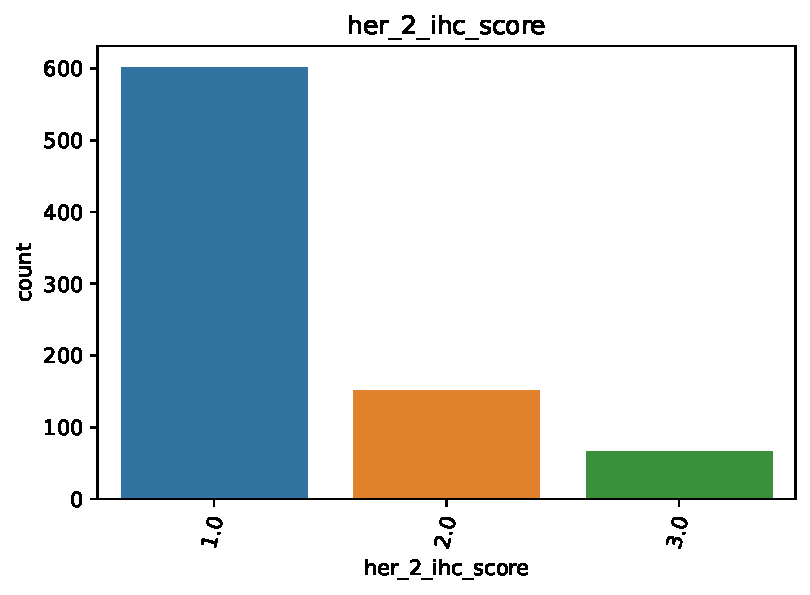
\includegraphics[width=1\linewidth]{NOTEBOOK/IMAGENES_DESCRIPTIVAS/21_her_2_ihc_score}\end{center}
			\\ \hline
			
			%------------------------------------------------------	
			Neoplasm Histologic Type Name
			& El \textit{Nombre del tipo histológico de neoplasia}, se visualiza en orden descendente de la siguiente manera: En primer lugar, 602 pacientes presentan \textit{Carcinoma Ductal Invasivo (IDC)} también llamado \textit{Carcinoma Ductal Infiltrante}. En segundo lugar, 143 pacientes presentan \textit{Carcinoma Lobulillar Invasivo (ILC)} también llamado \textit{Carcinoma Lobulillar Infiltrante.} En tercer lugar, 28 pacientes presentan otro tipo de neoplasia. En cuarto lugar, 23 pacientes presentan \textit{Tumores o Neoplasia mixta (MTCB)}, es decir conformada por los tipos de cáncer LBC e IDC. En quinto lugar, 14 pacientes presentan \textit{Carcinoma Mucinoso (MBC)}. En quinto lugar, 5 pacientes presentan \textit{Carcinoma Medular (MC)}. En sexto lugar, 3 pacientes presentan \textit{Carcinoma Metaplastico (MMC)}.
			& \begin{center}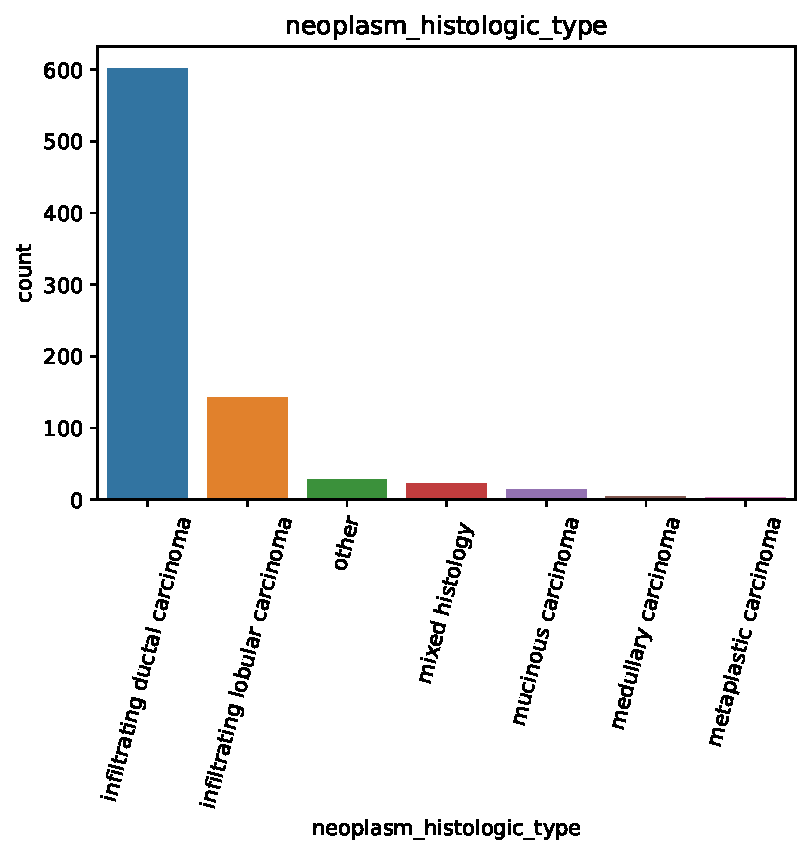
\includegraphics[width=1\linewidth]{NOTEBOOK/IMAGENES_DESCRIPTIVAS/22_neoplasm_histologic_type}\end{center}
			\\ \hline
		\end{tabular}
	\end{threeparttable}
\end{table*}

\begin{table*}[!htb]
	\footnotesize
	\begin{threeparttable}
		\begin{tabular}{p{2.5cm} p{7cm} p{6.5cm}} \toprule
			%------------------------------------------------------	
			Neoadjuvant Therapy Type Administered Prior To Resection Text
			& El \textit{Tratamiento neoadyuvante del paciente} se clasifica de forma nominal en dos categorías: La primera categoría corresponde al estado \textit{No} en donde se encuentran 809 pacientes que no recibieron un tratamiento inicial antes del tratamiento principal y la segunda categoría corresponde al estado \textit{Si} en donde se encuentran 9 pacientes a los cuales se les realizó un tratamiento inicial como quimioterapia, radioterapia o terapia hormonal para reducir el tamaño del tumor antes del tratamiento principal que generalmente consiste en cirugía.
			& \begin{center}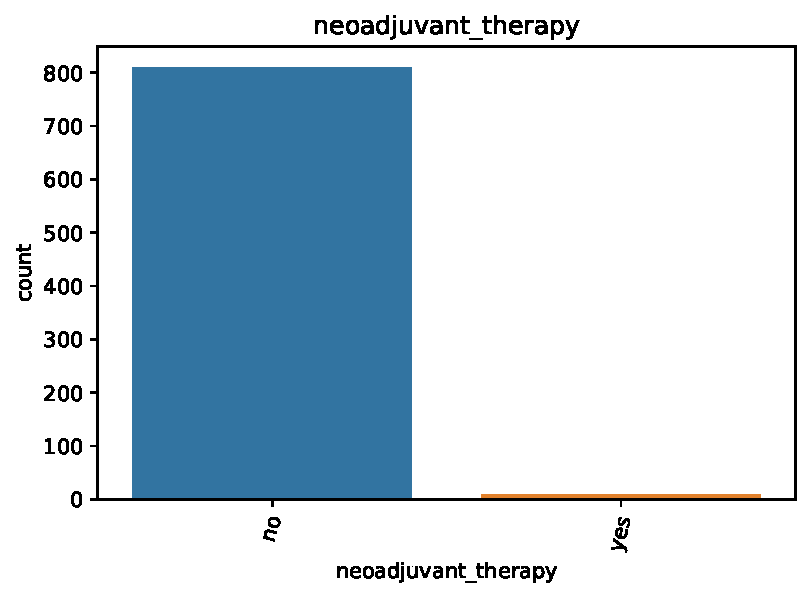
\includegraphics[width=1\linewidth]{NOTEBOOK/IMAGENES_DESCRIPTIVAS/23_neoadjuvant_therapy}\end{center}
			\\ \hline
			
			%------------------------------------------------------	
			ICD-10 Classification
			& El \textit{Diagnóstico de cáncer de mama por medio de la décima revisión ICD} se visualiza en orden descendente de la siguiente manera: En primer lugar, 810 pacientes presentan el código \textit{C50.9} el cual corresponde a una neoplasia maligna de sitio no especificado en la mama derecha. En segundo lugar, 3 pacientes presentan el código \textit{C50.3} el cual corresponde a una neoplasia maligna de cuadrante inferior interno de la mama derecha. En tercer lugar, 2 pacientes presentan el código \textit{C50.4} el cual corresponde a una neoplasia maligna de cuadrante superior externo de la mama derecha. En cuarto lugar, 1 paciente presentan el código \textit{C50.5} el cual corresponde a una neoplasia maligna de cuadrante superior interno de la mama derecha. En quinto lugar, 1 paciente presentan el código \textit{C50.2} el cual corresponde a una neoplasia maligna de cuadrante inferior externo de la mama derecha. En sexto lugar, 1 paciente presentan el código \textit{C50.8} el cual corresponde a una neoplasia maligna de sitios superpuestos de la mama derecha.
			
			& \begin{center}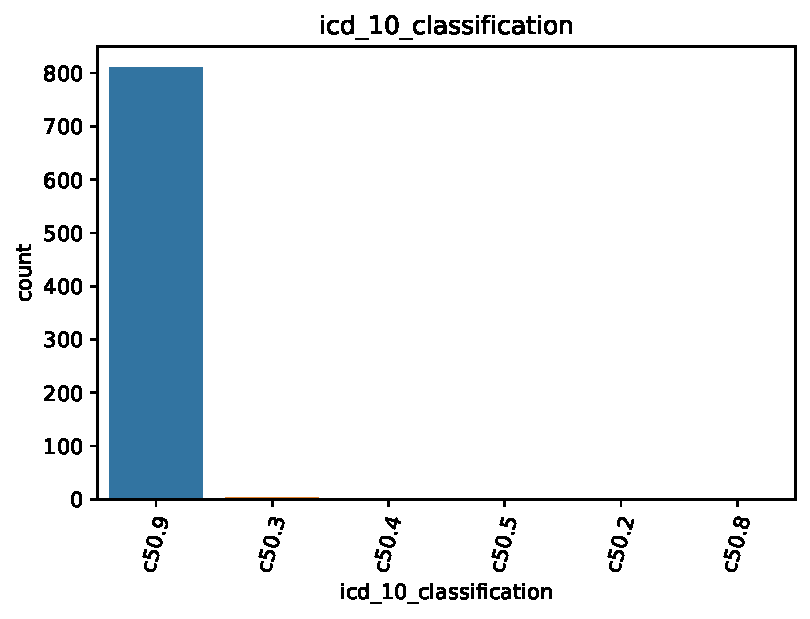
\includegraphics[width=1\linewidth]{NOTEBOOK/IMAGENES_DESCRIPTIVAS/25_icd_10_classification}\end{center}
			
			\begin{center}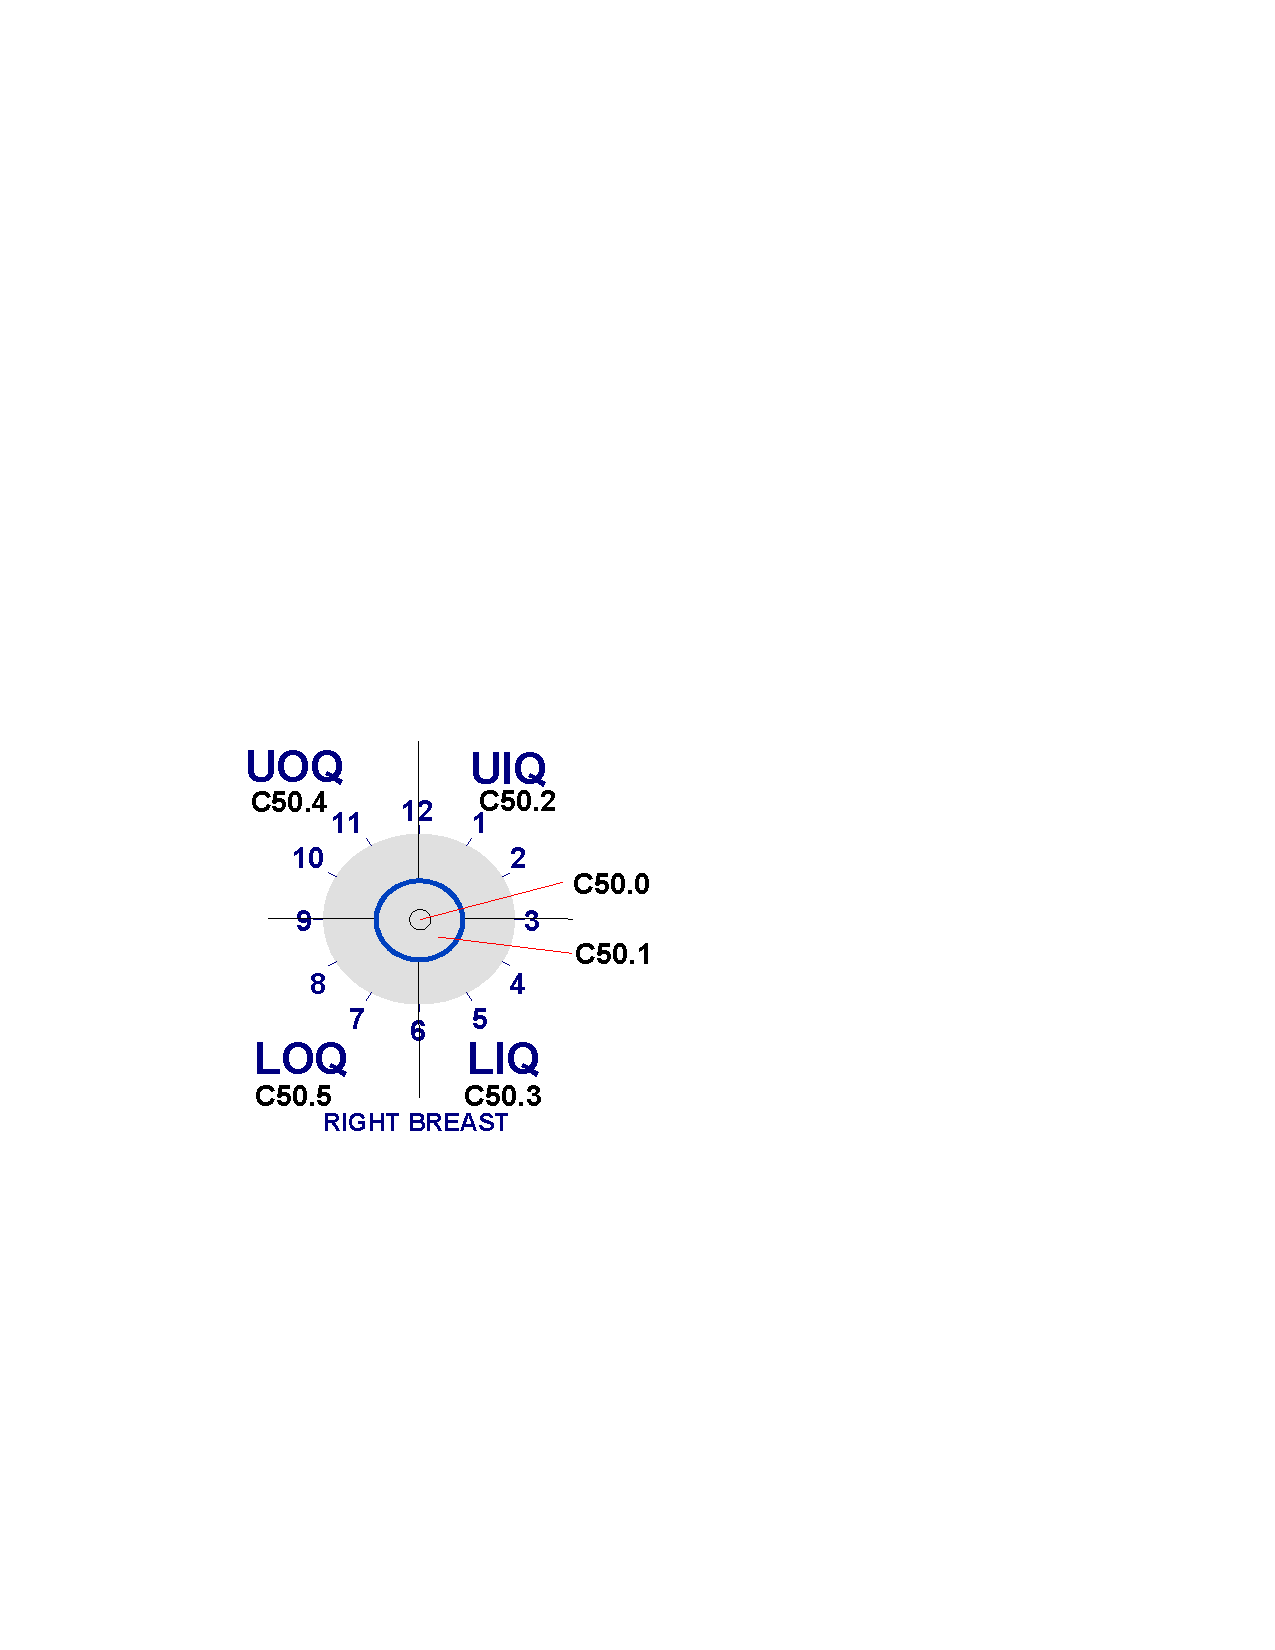
\includegraphics[width=0.75\linewidth]{NOTEBOOK/IMAGENES_DESCRIPTIVAS/25_icd_Breast_Clock_Position}\end{center}
			\\ \hline
			
			%------------------------------------------------------	
			IHC-HER2
			& El \textit{Estado de HER2 según la prueba de inmunohistoquímica (IHC)}, se visualiza en orden descendente de la siguiente manera: En primer lugar, 552 pacientes presentan un estado \textit{negativo}, es decir el cáncer no es posible tratarlo con medicamentos que tienen a la proteína HER2 como blanco. En segundo lugar, 145 pacientes presentan un estado \textit{ambiguo} esto significa que el estado de HER2 del tumor no está claro y es necesario hacer una prueba del estado FISH para clarificar el resultado. En tercer lugar, 121 pacientes presentan un estado \textit{positivo}, es decir el cáncer es posible tratarlo con medicamentos que tienen a la proteína HER2 como blanco.
			& \begin{center}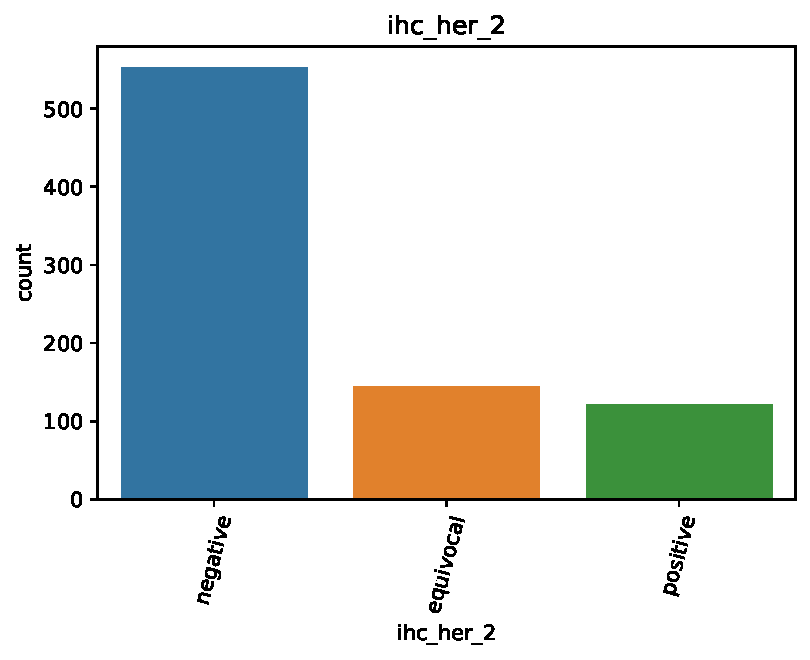
\includegraphics[width=1\linewidth]{NOTEBOOK/IMAGENES_DESCRIPTIVAS/26_ihc_her_2}\end{center}
			\\ \hline
		\end{tabular}
	\end{threeparttable}
\end{table*}

\begin{table*}[!htb]
	\footnotesize
	\begin{threeparttable}
		\begin{tabular}{p{2.5cm} p{7cm} p{6.5cm}} \toprule
			%------------------------------------------------------	
			Year Cancer Initial Diagnosis
			& El intervalo de años para el \textit{Diagnóstico Patológico inicial del cáncer} tiene una tendencia central aproximada en el año 2009, en donde el año de diagnóstico mínimo presentado es 1998 y año de diagnóstico máximo presentado es 2013.
			
			& \begin{center}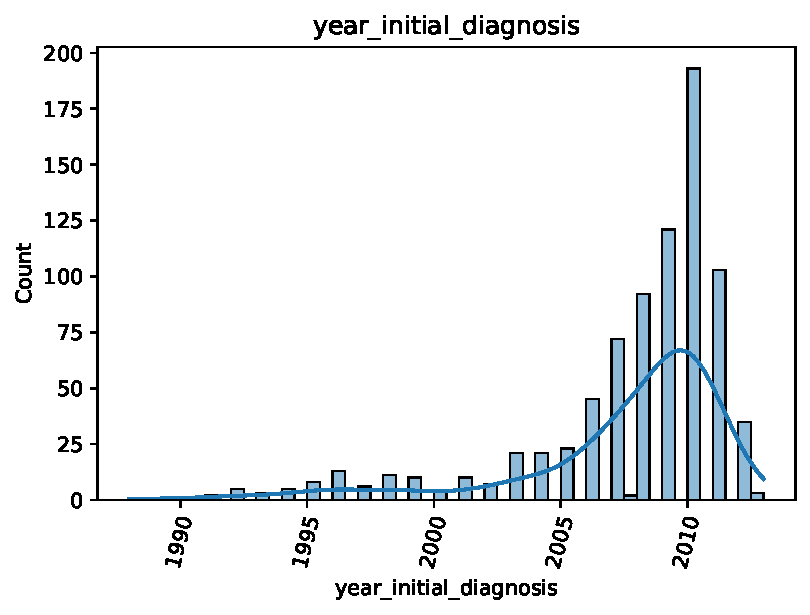
\includegraphics[width=1\linewidth]{NOTEBOOK/IMAGENES_DESCRIPTIVAS/27_year_initial_diagnosis}\end{center}
			\\ \hline
			
			%------------------------------------------------------	
			Primary Lymph Node Presentation Assessment Ind-3
			& La \textit{Evaluación de los ganglios linfáticos} en la presentación primaria de la enfermedad se clasifica de forma nominal en dos categorías: La primera categoría corresponde al estado \textit{Si} en donde se encuentran 798 pacientes en los que el oncólogo detecto la presencia de enfermedad metastásica en los ganglios linfáticos axilares y la segunda categoría al estado \textit{No} en donde se encuentran 20 pacientes en los que el oncólogo no detecto la presencia de enfermedad metastásica.
			
			& \begin{center}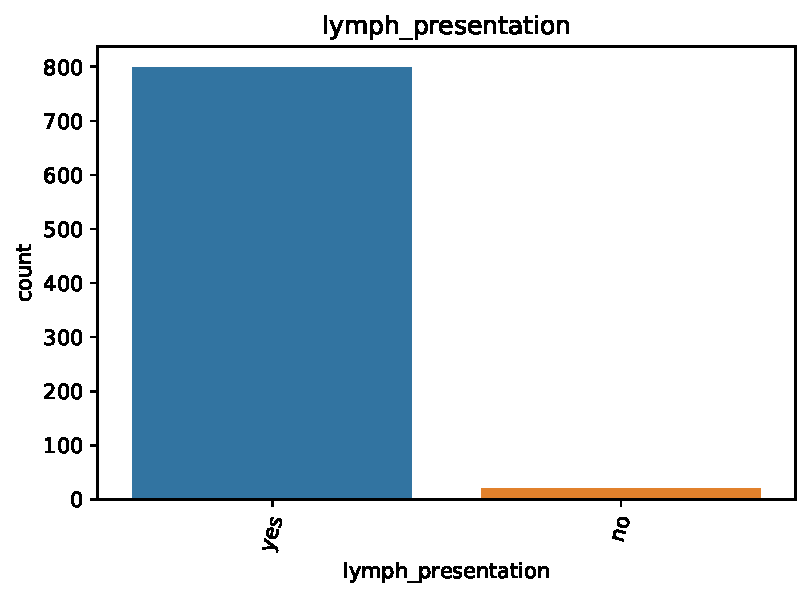
\includegraphics[width=1\linewidth]{NOTEBOOK/IMAGENES_DESCRIPTIVAS/28_lymph_presentation}\end{center}
			\\ \hline
			
			%------------------------------------------------------	
			Positive Finding Lymph Node Hematoxylin and Eosin Staining Microscopy Count
			& El \textit{Recuento de ganglios linfáticos positivos identificados mediante microscopía óptica con tinción de hematoxilina y eosina (H\&E)} tiene una tendencia central aproximada de 5 ganglios linfáticos con estado positivo, es decir que la tinción de hematoxilina presento una mayor proporción evidenciando la presencia de un tumor en crecimiento. Adicionalmente, se puede observar que  el valor mínimo ganglios linfáticos afectados fue 1 y el valor máximo de ganglios linfáticos afectados fue 34. 
			& \begin{center}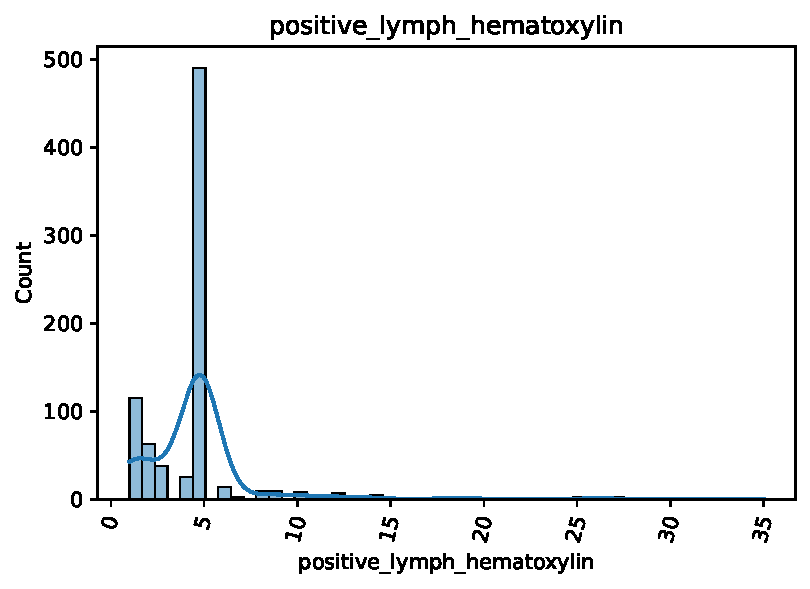
\includegraphics[width=1\linewidth]{NOTEBOOK/IMAGENES_DESCRIPTIVAS/29_positive_lymph_hematoxylin}\end{center}
			\\ \hline
			
			%------------------------------------------------------	
			Lymph Node(s) Examined Number
			& El número de \textit{ganglios linfáticos extirpados} y evaluados patológicamente para la enfermedad tiene una tendencia central aproximada de 10 ganglios linfáticos extirpados , en donde el número mínimo de ganglios linfáticos extirpados es 1 y el número máximo de ganglios linfáticos extirpados es 44.
			& 
			\begin{center}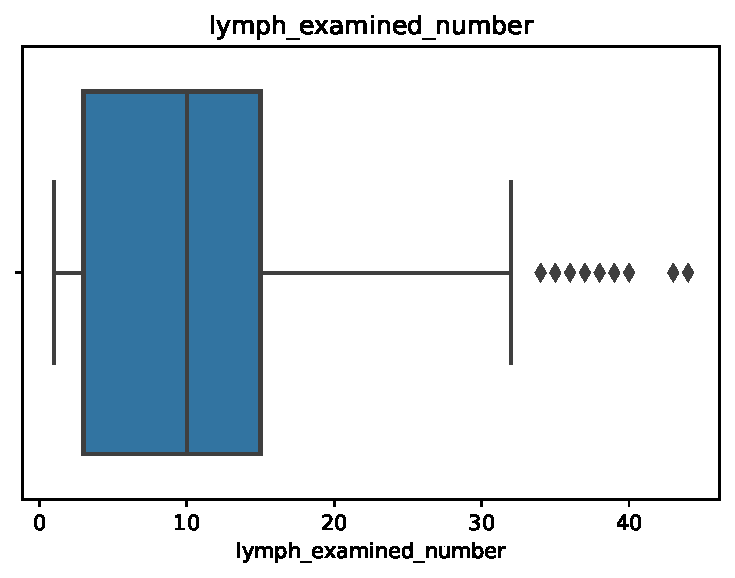
\includegraphics[width=1\linewidth]{NOTEBOOK/IMAGENES_DESCRIPTIVAS/31_lymph_examined_number}\end{center}
			\\ \hline
		\end{tabular}
	\end{threeparttable}
\end{table*}

\begin{table*}[!htb]
	\footnotesize
	\begin{threeparttable}
		\begin{tabular}{p{2.5cm} p{7cm} p{6.5cm}} \toprule
			%------------------------------------------------------	
			Menopause Status
			& El \textit{estado de la menopausia}, se visualiza en orden descendente de la siguiente manera: En primer lugar, 593 pacientes presentan un estado de \textit{PostMenopausia}, en el cual los niveles hormonales permanecen bajos y ya no se presenta un período mensual debido a que los ovarios han dejado de liberar óvulos. En segundo lugar, 166 pacientes presentan un estado de \textit{PreMenopausia}, en el cual la reserva ovárica empieza a disminuir y la mujer pierde su fertilidad. Suele iniciarse sobre los 40 años y tener una duración muy variable, desde pocos años hasta 10 o más. En tercer lugar, 59 pacientes presentan un estado de \textit{PeriMenopausia} el cual se presenta en una etapa más corta que precede a la menopausia y dura hasta los 12 meses posteriores de la última menstruación. Suele durar unos 2 o 3 años y se caracteriza por las irregularidades en el ciclo menstrual. La edad más habitual en la que se presenta la perimenopausia es entre los 45 y los 50 años\cite{ReproAsistidaORG}.
			
			& \begin{center}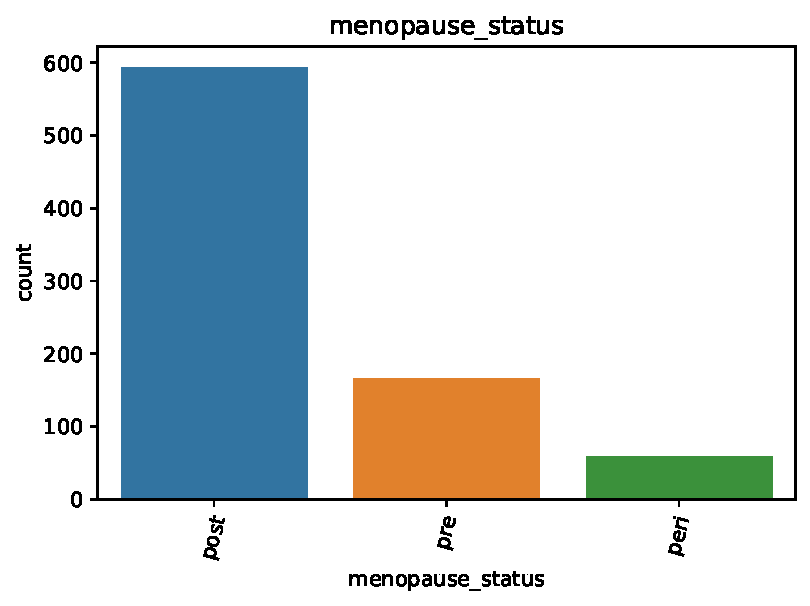
\includegraphics[width=1\linewidth]{NOTEBOOK/IMAGENES_DESCRIPTIVAS/32_menopause_status}\end{center}
			  \begin{center}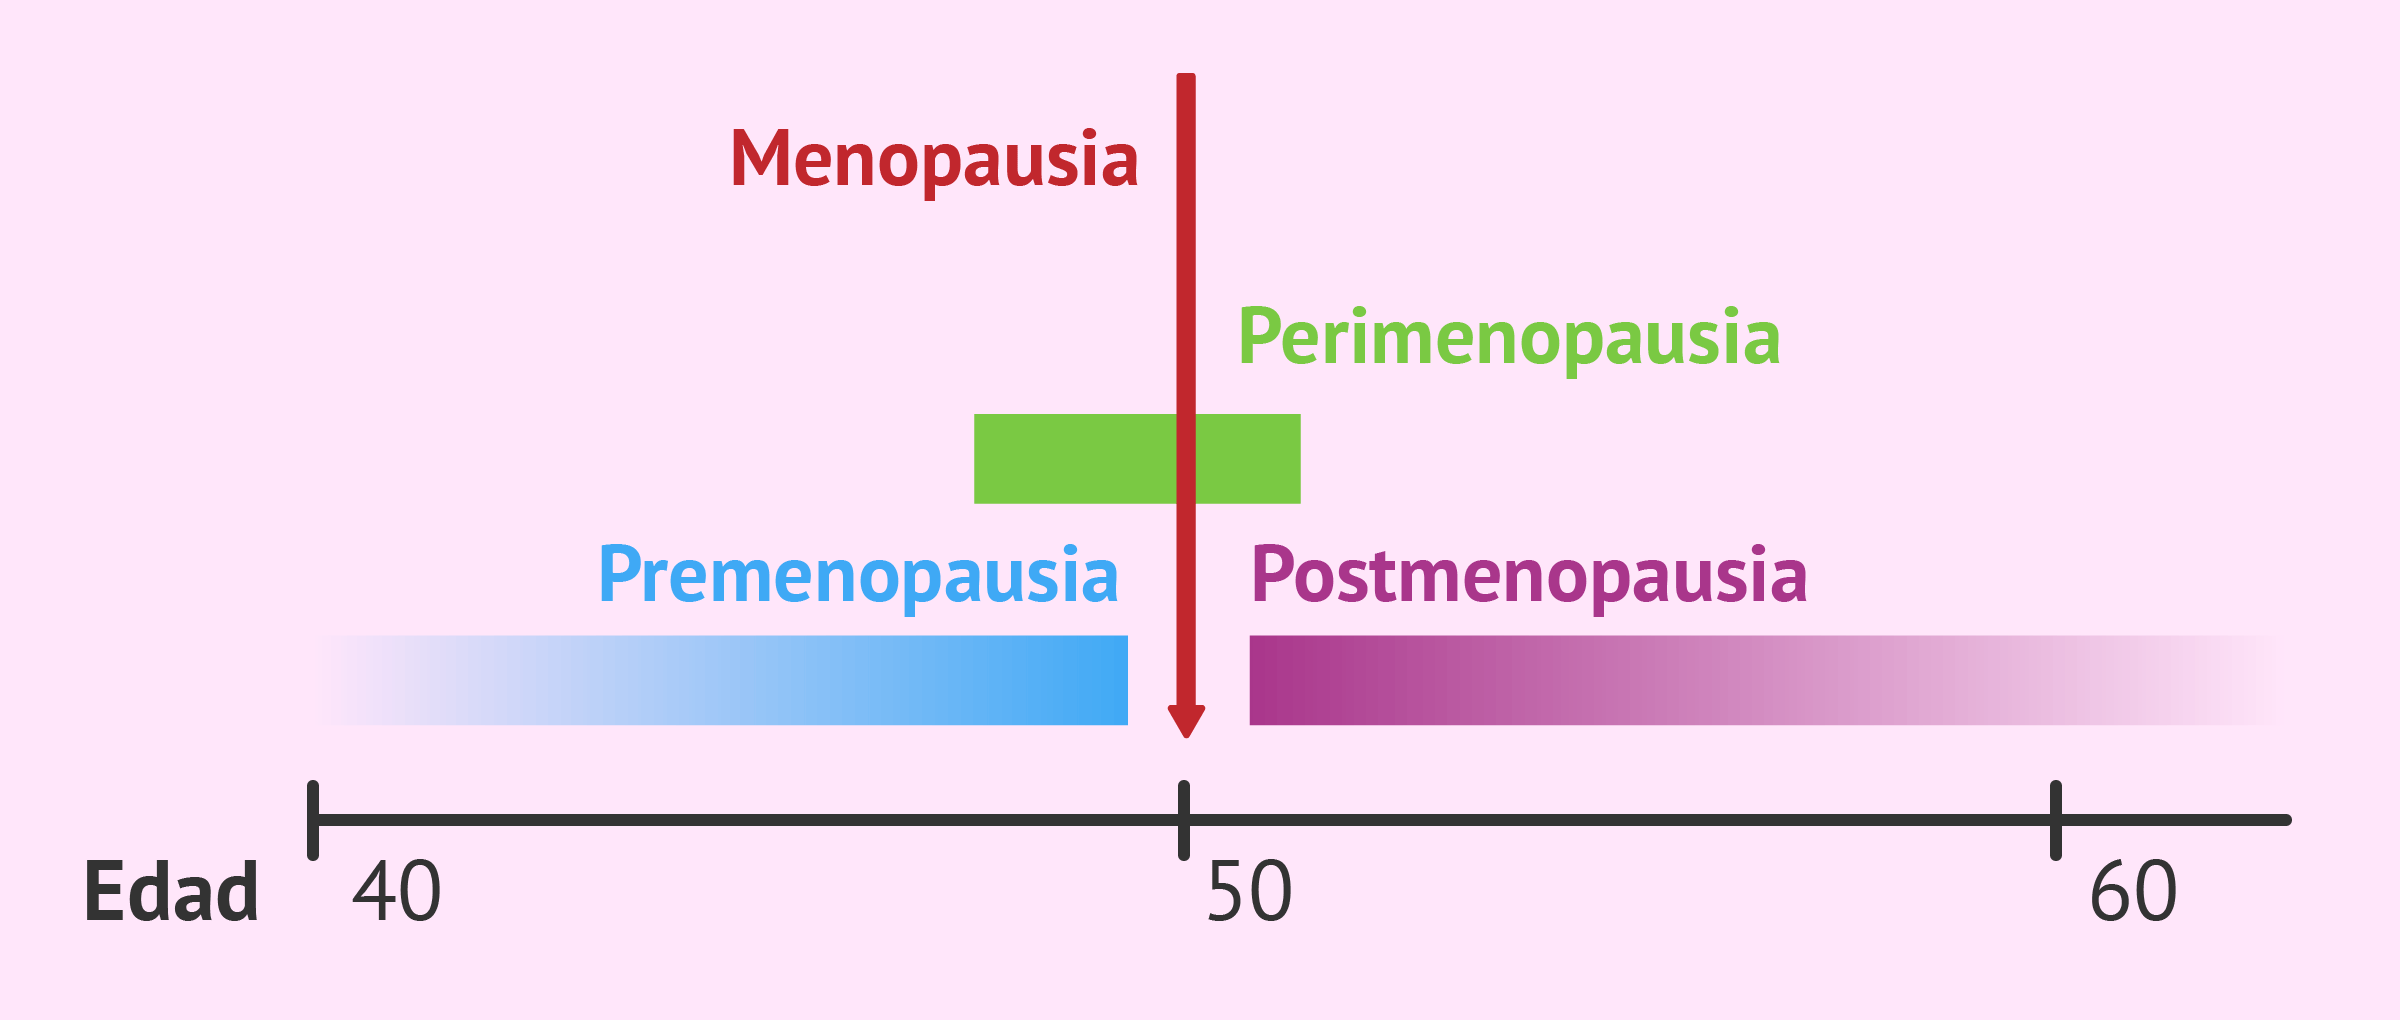
\includegraphics[width=1\linewidth]{IMAGENES/menopausia}\end{center}
			\\ \hline
			
			%------------------------------------------------------	
			Variable
			& Descripcion
			
			& \begin{center}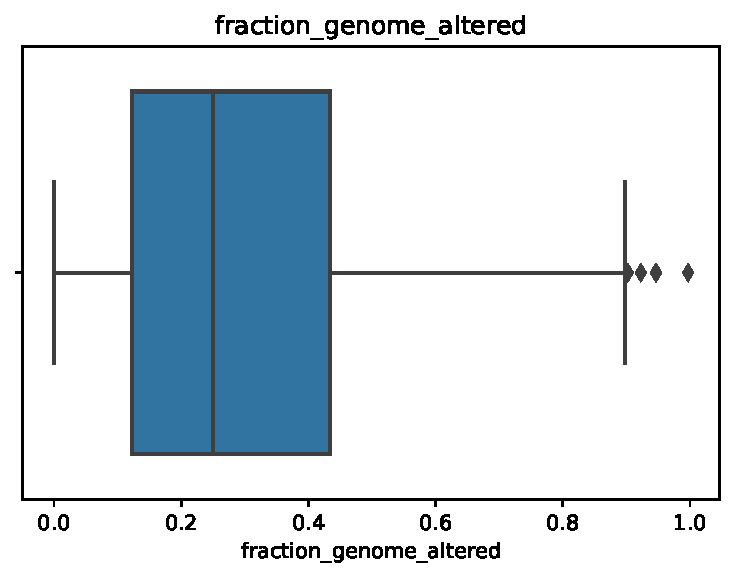
\includegraphics[width=1\linewidth]{NOTEBOOK/IMAGENES_DESCRIPTIVAS/17_fraction_genome_altered}\end{center}
			\\ \hline
			
			%------------------------------------------------------	
			Variable
			& Descripcion
			& \begin{center}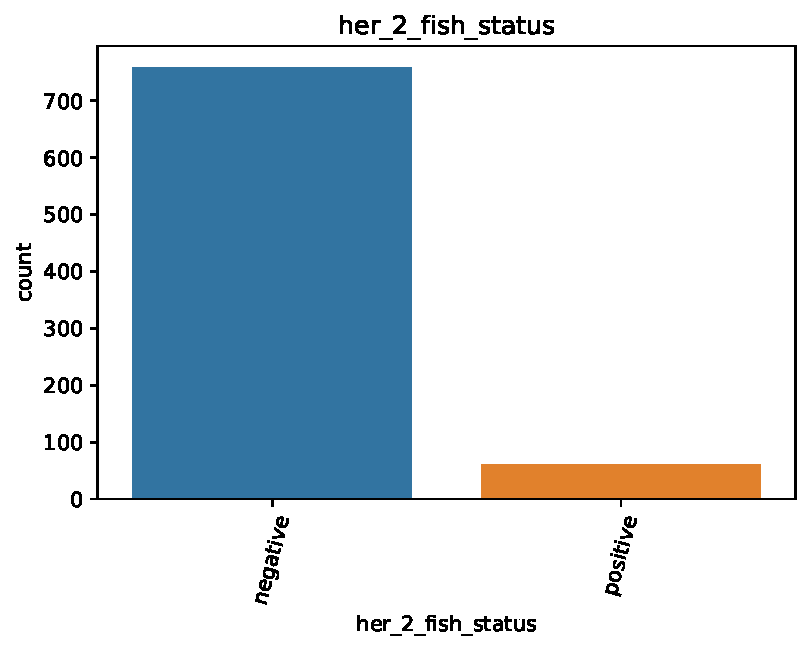
\includegraphics[width=1\linewidth]{NOTEBOOK/IMAGENES_DESCRIPTIVAS/19_her_2_fish_status}\end{center}
			\\ \hline
		\end{tabular}
	\end{threeparttable}
\end{table*}








\clearpage
\section{Fase 6: Modelado y Ejecución}
En esta fase, el científico de datos diseña, crea o utiliza un modelo predictivo o descriptivo y lo alimenta con la versión del conjunto de datos o imágenes obtenidos en la fase de procesamiento y transformación. En esta fase, el científico debe seleccionar el tipo de aprendizaje (supervisado, no supervisado y por refuerzo) y la técnica determinada (regresión, clasificación, clustering, CNN, RNN, etc.) acorde a las preguntas planteadas en el \textit{BCQM}. Hay que mencionar que en esta fase el \textit{Data Analysis Team} debe definir junto al médico experto en oncología la tolerancia de error permitida en el modelo, esto dado a que la sensibilidad de los análisis puede variar dependiendo del tipo de cáncer de mama y la técnica de diagnóstico. Es probable que el científico de datos pruebe múltiples algoritmos con sus respectivos parámetros para encontrar el mejor modelo para las variables oncológicas disponibles. Cabe resaltar, que es de vital importancia que los modelos propuestos no tengan problemas de sobreajuste o infra ajuste ya que esto puede generar resultados erróneos o poco significativos. Adicionalmente, el científico de datos en cuestión junto al \textit{Data Analysis Team} deben definir la infraestructura a nivel de servidor necesaria para el entrenamiento y prueba del modelo según la cantidad de información a procesar, esto con el propósito de generar resultados acertados en el menor tiempo posible en pro de cumplir las tareas definidas en la fase de planeación de actividades y dar valor a los datos oncológicos una vez finalice el \textit{Release}.

\subsection{Agrupamiento(Clustering)}
Ahora bien, dado que las preguntas sobre el cáncer de mama planteadas en el BCQM se basan en datos de origen genómico y por ende tienen una representación simbólica con atributos cuantitativos y/o cualitativos en este caso de estudio se requiere un \textit{análisis diagnostico} para determinar las causas de las tendencias y las correlaciones entre las 41 variables oncológicas. Por lo tanto, se seleccionó el método de agrupamiento(\textit{Clustering}), ya que nos permite reunir los datos genómicos en clases o \textit{clusters} basados en los tipos de cáncer lobulillar invasivo(ILC) o ductal invasivo(IDC), de tal forma que es posible identificar que las variables de un determinado cluster tengan una similaridad alta o baja con respecto a los demás clusters.

Dado lo anterior, en la tabla \ref{Clustering_Models} se observan los algoritmos de agrupamiento que fueron ejecutados para posteriormente seleccionar el de mejor desempeño. Para ejecutarlos, se utilizó el lenguaje multiparadigma \textit{Python} y la librería \textit{scikit-learn}, ya que permiten agilizar el entrenamiento de algoritmos de aprendizaje no supervisado.
\\\\
En este caso se realizó el análisis con base al agrupamiento de la totalidad de datos conformado por $818$ filas y $41$ columnas. Simultáneamente, para optimizar el modelo se utilizó el $95\%$ de los datos para el entrenamiento y el $5\%$ de datos restante para comprobar la precisión del agrupamiento y así poder de analizar los clusters generados. Cabe resaltar, que para la creación, entrenamiento y prueba del modelo se utilizó una maquina equipada con un procesador Intel Core i7-11370H de 11th generación con una frecuencia de 3.30 GHz-4.9 GHz , una tarjeta NVIDIA GeForce RTX 3050, un disco duro SSD Samsung con una velocidad de lectura de 7,000 MB/s y 48GB de memoria RAM. 

Para obtener el modelo de agrupamiento más adecuado, se utilizaron las métricas de validación interna basadas en el índice de \textit{Davies-Bouldin} y el \textit{Coeficiente de silhouette}. Además, también se validó la cantidad de clusters generados para evaluar la eficacia en el agrupamiento de los datos. El resultado de este análisis puede ser observado en la figura \ref{TSNE}, la cual fue generada con el método T-SNE \footnote{T-SNE: T-distributed Stochastic Neighbor Embedding}, el cual genera una distribución de probabilidad que representa las similitudes entre vecinos en un espacio de gran dimensión y en un espacio de menor dimensión. 

Llegados a este punto, los modelos de agrupación \textit{Espectral(Spectral)} y \textit{Desplazamiento medio(Mean Shift)}  fueron los que presentaron un mayor valor en el coeficiente de Silhouette y un menor valor en el índice da Davies-Bouldin, respectivamente. Sin embargo al observar en la gráfica T-SNE del modelo de agrupación \textit{Espectral}, se pueden identificar 2 clusters, en donde el Cluster 0 abarca aproximadamente el 99\% del espacio con respecto al Cluster 1, por lo que en no existe una cohesión ni una separación clara de los datos. De la misma manera, el modelo de \textit{desplazamiento medio} presenta un comportamiento similar que aunque no se observa la gráfica T-SNE puede ser comprobado en la figura \ref{distance} que representa la distancia entre clusters con respecto a la posición inicial.

Finalmente, el modelo seleccionado para analizar el comportamiento de conjunto de datos del carcinoma invasivo de mama (TCGA, Cell 2015), fue el de \textit{agrupación BIRCH}, ya que no solo genero un coeficiente de silhouette y un índice de Davies-Bouldin congruente sino también al validar la gráfica T-SNE se visualiza que los clusters presentan una métrica de cohesión y separación idónea.

\begin{table*} [!htb]
	\footnotesize
	\begin{threeparttable}
		\caption{Modelos Machine Learning para agrupamiento (Clustering).}
		\label{Clustering_Models}
		\begin{tabular}{p{1cm} p{6cm} p{2.5cm} p{2.5cm} p{1.5cm}} \toprule	
			\begin{center}Id\end{center}
			&\begin{center}Modelo Clustering\end{center}
			&\begin{center}Silhouette\end{center}
			&\begin{center}Davies-Bouldin\end{center}
			&\begin{center}Clusters\end{center}
			\\ \hline 1 & K-Means Clustering 	&	0,0826	&	2,5179	&	4
			\\ \hline 2 & Affinity Propagation	&	0,0518	&	2,2123	&	68
			\\ \hline 3 & Mean Shift Clustering 	&	0,2790	&	1,2792	&	7
			\\ \hline 4 & Spectral Clustering	&	0,7986	&	0,1419	&	2
			\\ \hline 5 & Agglomerative Clustering	&	0,1034	&	2,0468	&	4
			\\ \hline 6 & DB Spatial Clustering 	&	0,0000	&	0,0000	&	-1
			\\ \hline 7 & OPTICS Clustering	&	-0,2044	&	1,9565	&	10
			\\ \hline 8 & BIRCH Clustering	&	0,1286	&	1,8703	&	4
			\\ \hline 9 & K-Modes Clustering	&	0,0547	&	3,8189	&	3
			\\ \hline
		\end{tabular}
	\end{threeparttable}
\end{table*}

\begin{figure} 
	\setlength\tabcolsep{3pt}%%
	\centering
	\caption{Modelos Clustering aplicados al conjunto de datos del Carcinoma invasivo de mama (TCGA, Cell 2015).}
	\label{TSNE}
	\begin{tabular}{|c|c|}
		\hline
		\textbf{K-Means} &
		\textbf{Affinity Propagation} \\
		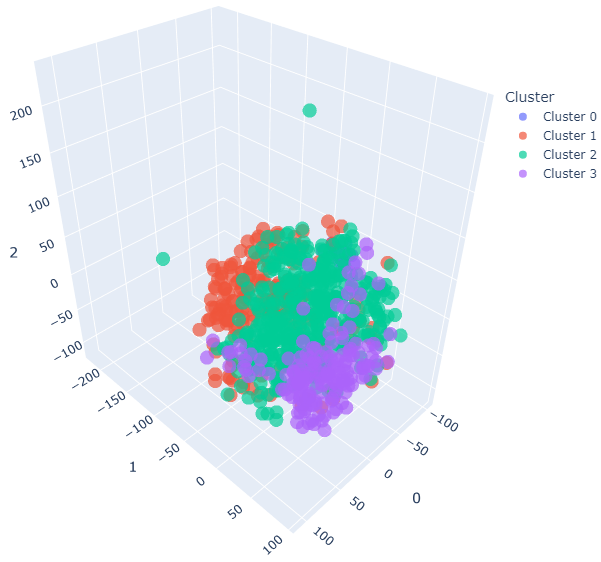
\includegraphics[width=0.5\textwidth]{NOTEBOOK/IMAGENES_CLUSTERING/1_TNSE_Kmeans} &
		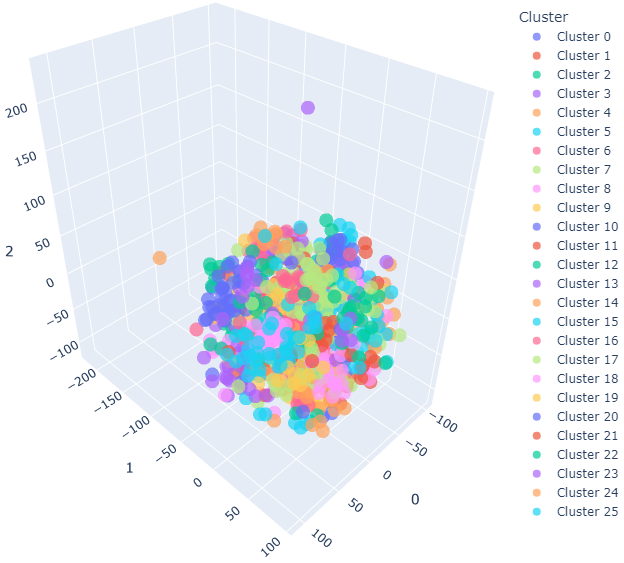
\includegraphics[width=0.5\textwidth]{NOTEBOOK/IMAGENES_CLUSTERING/2_TNSE_Affinity_Propagation} \\
		\hline
		
		\textbf{Mean Shift Clustering} &
		\textbf{Spectral Clustering} \\
		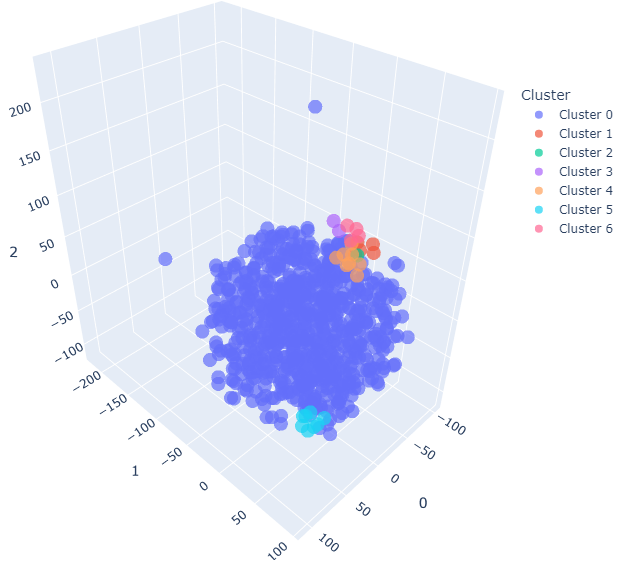
\includegraphics[width=0.5\textwidth]{NOTEBOOK/IMAGENES_CLUSTERING/3_TNSE_Mean_Shift_Clustering} &
		\includegraphics[width=0.5\textwidth]{NOTEBOOK/IMAGENES_CLUSTERING/4_TNSE_Spectral_ Clustering} 
		\\ \hline
	\end{tabular}
\end{figure}

\begin{figure} 
	\setlength\tabcolsep{3pt}%%
	\centering
	\begin{tabular}{|c|c|}
		\hline
		\textbf{Agglomerative Clustering} &
		\textbf{Density-Based Spatial Clustering} \\
		\includegraphics[width=0.5\textwidth]{NOTEBOOK/IMAGENES_CLUSTERING/5_TNSE_Agglomerative_Clustering} &
		\includegraphics[width=0.5\textwidth]{NOTEBOOK/IMAGENES_CLUSTERING/6_TNSE_Density_Based_Spatial_Clustering} 
		\\ \hline
		\textbf{OPTICS Clustering} &
		\textbf{BIRCH Clustering} \\
		\includegraphics[width=0.5\textwidth]{NOTEBOOK/IMAGENES_CLUSTERING/7_TNSE_OPTICS_Clustering} &
		\includegraphics[width=0.5\textwidth]{NOTEBOOK/IMAGENES_CLUSTERING/8_TNSE_Birch_Clustering} 
		\\ \hline
	\end{tabular}
	\begin{tabular}{|c|}
		\hline
		\textbf{K-Modes Clustering} \\
		\includegraphics[width=0.5\textwidth]{NOTEBOOK/IMAGENES_CLUSTERING/9_TNSE_Kmodes}
		\\ \hline
	\end{tabular}
\end{figure}


\begin{figure} 
	\setlength\tabcolsep{3pt}%%
	\centering
	\caption{Mapas de distancia entre clusters de los modelos aplicados al conjunto de datos del carcinoma invasivo de mama (TCGA, Cell 2015).}
	\label{distance}
	\begin{tabular}{|c|c|}
		\hline
		\textbf{K-Means} &
		\textbf{Affinity Propagation} \\
		\includegraphics[width=0.5\textwidth]{NOTEBOOK/IMAGENES_CLUSTERING/1_MAP_Kmeans} &
		\includegraphics[width=0.5\textwidth]{NOTEBOOK/IMAGENES_CLUSTERING/2_MAP_Affinity_Propagation} 
		\\ \hline
	\end{tabular}
	\begin{tabular}{|c|}
		\hline
		\textbf{Mean Shift Clustering} \\
		\includegraphics[width=0.5\textwidth]{NOTEBOOK/IMAGENES_CLUSTERING/3_MAP_Meanshift_Distance}
		\\ \hline
	\end{tabular}
\end{figure}



\section{Fase 7: Evaluación e Interpretación}
En esta fase, el \textit{Data Analysis Team} evalúa el modelo para comprender su calidad y garantizar que este aborda las preguntas generadas en el \textit{BCQM} de manera adecuada y completa. Es necesario que para realizar la evaluación se utilicen medidas especializadas basadas en el rendimiento, sensibilidad y especificidad del modelo. Adicionalmente, los resultados obtenidos deben ser entendibles por el medico experto en oncología, en donde se garantice que dichos resultados sean interpretados correctamente y estén relacionados a la estadificación y los biomarcadores del cáncer de mama. Es importante que el medico junto al científico de datos ajusten el modelo según las necesidades. Dado que se esta trabajando con datos médicos sensibles, es necesario que al modelo final se aplique a un conjunto de validación para realizar una evaluación final. Además, el \textit{Data Analysis Team} puede asignar al modelo pruebas de \textit{significancia estadística} como prueba adicional para comprobar la respuesta obtenida a la pregunta generada. Esta prueba adicional es fundamental para justificar la implementación del modelo. Finalmente, dado que en el \textit{BCQM} se pueden plantear múltiples preguntas relacionadas a diferentes tipo de cáncer de mama y técnicas de diagnostico durante el \textit{Release}, es necesario que los científicos con ayuda del ingeniero de datos unan, si es posible, los resultados obtenidos en una matriz o mapa de calor para identificar el coeficiente de correlación entre dos o mas variables oncológicas. Esta matriz resultante debe ser analizada por el medico experto en oncología para determinar si existe una relación significativa entre los diferentes tipos de cáncer de mama.
\section{Fase 8: Retroalimentación medica }
En esta fase, el medico experto en oncología determina si los resultados generados por el modelo de ML o DL lograron responder las preguntas planteadas en el \textit{BCQM} y si la nueva información obtenida es suficiente para diagnosticar el cáncer de mama o si dichos resultados generaron información relevante para determinar la causa u origen de esta enfermedad, en pocas palabras, si los datos analizados produjeron un valor agregado al dominio médico. En el caso de que los resultados obtenidos no lograsen dar valor a los datos, el \textit{Data Analysis Team} deberá decidir si es necesario replantear las preguntas o si se debe adquirir nuevos datos para ajustar el modelo generado. Además, el experto en compañía del científico y el ingeniero de datos, basado en su perspicacia médica, deberá ayudar a decidir cual estrategia es las más apropiada para generar resultados significativos. De forma similar, si el resultado fue satisfactorio el medico debe emitir un dictamen del \textit{nivel de impacto} que tuvo la información generada por los modelos al diagnosticar el padecimiento del cáncer de mama a un determinado paciente y una vez comprobada la información, junto al \textit{Data Analysis Team} alimentar el conjunto de datos con la información obtenida de los diagnósticos generados a cada individuo. Lo anterior con el propósito de mejorar el desempeño de los modelos existentes y aumentar su precisión. Finalmente, en cada \textit{Release} se debe garantizar que el tiempo de diagnóstico sea cada vez menor o que se genere nueva información que el medico pueda utilizar en sus funciones diarias y que ayude a determinar el origen, relación o posible tratamiento de esta enfermedad.

\subsection{Revisión de respuestas}
Para este caso de estudio, la retroalimentación medica se fundamentó en la investigación \textit{“Comprehensive Molecular Portraits of Invasive Lobular Breast Cancer”}\cite{Ciriello2015}, la cual se basa en el \textit {Atlas del Genoma del Cáncer} con el propósito de catalogar cambios moleculares de importancia biológica responsables de la aparición de cáncer haciendo uso de la secuenciación genómica. Dado lo anterior, a continuación se observa la comparación entre los resultados obtenidos por el \textit{Data Analysis Team} y el \textit{Ph.D Giovanni Ciriello} que en conjunto con el grupo de oncólogos e ingenieros de la tabla \ref{Molecular_Portraits} realizaron un análisis exhaustivo de muestras de tumores de mama en donde determinaron que el Carcinoma Lobulillar Invasivo(ILC) es una enfermedad molecularmente distinta con rasgos genéticos característicos, obteniendo información clave para la estratificación de las pacientes que puede permitir un seguimiento clínico más acertado. Cabe resaltar, que las muestras obtenidas para ambos análisis se generaron a partir de la Biopsia por aspiración con aguja fina (FNA) y Biopsia con aguja gruesa (CNB).
\begin{table*}[!htb]
	\footnotesize
	\centering
	\begin{threeparttable}
		\begin{tabular}{p{0.5cm} p{3.5cm} p{4cm} p{5.5cm}} \toprule
			\begin{center}\textit{N}\end{center}   
			&\begin{center}Investigador\end{center}       
			&\begin{center}Departamento\end{center}
			&\begin{center}Universidad\end{center}  
			%------------------------------------------------------	
			\\ \hline
			1
			& Giovanni Ciriello
			& Genética Médica
			& Universidad de Lausana (Suiza)
			%------------------------------------------------------	
			\\ \hline
			2
			& Michael L. Gatza
			& Centro Oncológico Integral Lineberger
			& Universidad de Carolina del Norte (EE.UU.)
			%------------------------------------------------------	
			\\ \hline
			3
			& Andrew H. Beck
			& Patología
			& Facultad de Medicina de Harvard (EE.UU.)
			%------------------------------------------------------
			\\ \hline
			4
			& Matthew D. Wilkerson
			& Genética Médica
			& Universidad de Carolina del Norte (EE.UU.)
			%------------------------------------------------------
			\\ \hline
			5
			& Suhn K. Rhie
			& Centro Oncológico Integral Norris
			& Universidad del Sur de California (EE.UU.)
			%------------------------------------------------------
			\\ \hline
			6
			& Alessandro Pastore
			& Programa de Biología Computacional
			& Centro de Cáncer Memorial Sloan Kettering (EE.UU.)
			%------------------------------------------------------
			\\ \hline
			7
			& Hailei Zhang
			& Instituto Eli y Edythe L.
			& Broad del MIT y Harvard (EE.UU.)
			%------------------------------------------------------
			\\ \hline
			8
			& Michael McLellan
			& Instituto del Genoma
			& Facultad de Medicina de la Universidad de Washington (EE.UU.)					
			%------------------------------------------------------
			\\ \hline
			9
			& Christina Yau
			& Biología del envejecimiento
			& Instituto Buck (EE.UU.)
			%------------------------------------------------------
			\\ \hline
			10
			& Cyriac Kandoth
			& Programa de Oncología Humana y Patogénesis
			& Centro de Cáncer Memorial Sloan Kettering (EE.UU.)
			%------------------------------------------------------
			\\ \hline
			11
			& Reanne Bowlby
			& Centro de Ciencias del Genoma Michael Smith
			& Agencia del Cáncer de BC (Canada)
			%------------------------------------------------------
			\\ \hline
			12
			& Hui Shen
			& Centro de Epigenética
			& Instituto de investigación Van Andel (EE.UU.)
			%------------------------------------------------------
			\\ \hline
			13
			& Sikander Hayat
			& Programa de biología computacional
			& Centro de Cáncer Memorial Sloan Kettering (EE.UU.)
			%------------------------------------------------------
			\\ \hline
			14
			& Robert Fieldhouse
			& Programa de biología computacional
			& Centro de Cáncer Memorial Sloan Kettering (EE.UU.)
			%------------------------------------------------------
			\\ \hline
			15
			& Susan C. Lester
			& Patología
			& Facultad de Medicina de Harvard (EE.UU.)
			%------------------------------------------------------
			\\ \hline
			16
			& Gary M.K. Tse
			& Patología Anatómica y Celular
			& Universidad China de Hong Kong (Hong Kong)
			%------------------------------------------------------
			\\ \hline
			17
			& Rachel E. Factor
			& Departamento de Patología
			& Universidad de Utah (EE.UU.)
			%------------------------------------------------------
			\\ \hline
			18
			& Laura C. Collins
			& Patología
			& Facultad de Medicina de Harvard (EE.UU.)
			%------------------------------------------------------
			\\ \hline
			19
			& Kimberly H. Allison
			& Patología
			& Universidad de Stanford (EE.UU.)
			%------------------------------------------------------
			\\ \hline
			20
			& Yunn-Yi Chen
			& Patología
			& Universidad de California (EE.UU.)
			%------------------------------------------------------
			\\ \hline
			20
			& Charles M. Perou
			& Centro Oncológico Integral Lineberger
			& Universidad de Carolina del Norte (EE.UU.)						
			\\ \hline	
		\end{tabular}
		\caption{Colaboradores de la investigación \textit{“Comprehensive Molecular Portraits of Invasive Lobular Breast Cancer”}.}
		\label{Molecular_Portraits}
	\end{threeparttable}
\end{table*}

%-------------------------------------------------------------
\clearpage
\alertinfo{\textbf{QU1:} ¿Presenta el Carcinoma Lobulillar Invasivo(ILC) características genéticas molecularmente diferentes a los demás tipos de cáncer de mama?}
\begin{itemize}[label=\PencilRightDown]
	\item \textbf{Data Analysis Team:} En el cáncer ILC las variables genéticas presentaron un comportamiento diferente en comparación con el cáncer IDC y MTCB. Para ser más específicos en la estadificación por neoplasia del ganglio linfático el cáncer ILC presenta una mayor afectación y/o propagación hacia los ganglios linfáticos axilares cercanos al seno afectado. De manera similar, presenta un tamaño tumoral aproximadamente 2 veces más grande que el cáncer IDC y una frecuencia de aparición mayor. Adicionalmente, se identifica una afectación metastásica constante en una cantidad considerable de ganglios linfáticos. Por otra parte, el recuento de mutaciones del ILC en el ADN presenta un menor grado de crecimiento de las células sanas y se divide de una forma tardía en comparación con el cáncer IDC el cual presenta una propagación más rápida, una tasa de supervivencia menor en los pacientes y un crecimiento acelerado del tejido mamario que dificulta la localización, visibilidad y diagnóstico del ILC. Por último, los pacientes con ILC tienen un valor bajo de carga mutacional tumoral (TMB), es decir que generan una menor cantidad de neoantígenos, lo que hace que los tumores sean menos inmunogénicos a los tratamientos. Dado lo anterior, es plausible afirmar que el cáncer ILC presenta características genéticas diferentes a los demás tipos de carcinoma invasivo. 
	
	\item \textbf{Ph.D Giovanni Ciriello:} En este estudio se analizaron varios tumores de mama, en donde se identificaron como características enriquecidas del ILC, la pérdida de cadherina-E y mutaciones genéticas en las proteínas PTEN, TBX3 y FOXA1. La pérdida de PTEN se asoció con un aumento de la fosforilación de AKT, que fue mayor en el cáncer ILC en comparación con los demás tipos de cáncer de mama. Las mutaciones se correlacionaron con una mayor expresión y actividad de FOXA1. Por el contrario, las mutaciones de GATA3 y su elevada expresión caracterizaron al tipo de cáncer IDC luminal A, lo que sugiere una modulación diferencial de la actividad del receptor ER positivo en los tipos de cáncer ILC e IDC. Las firmas relacionadas con la proliferación y el sistema inmunitario determinaron tres subtipos de ILC asociados a diferencias en la supervivencia. Este estudio identificó múltiples alteraciones genómicas que discrepan entre ILC e IDC, demostrando a nivel molecular que el ILC es un subtipo distinto de cáncer de mama y proporcionando nuevos conocimientos sobre su biología tumoral y las opciones terapéuticas. Dado lo anterior, se infiere que el cáncer ILC es una enfermedad clínica y molecularmente distinta\cite{Ciriello2015}.
\end{itemize}

\clearpage
\alertinfo{\textbf{QU2:} ¿Es la proteína HER2 positiva un rasgo genético necesario para diagnosticar el Carcinoma Ductal invasivo(IDC) pero no suficiente para diagnosticar el Carcinoma Lobulillar Invasivo(ILC)?}

\begin{itemize}[label=\PencilRightDown]
	\item \textbf{Data Analysis Team:} El Porcentaje positivo de HER2 según la prueba de inmunohistoquímica (IHC) presento una diferencia en los pacientes con IDC ya que el 91,06\% obtuvieron una tinción de membrana apenas perceptible, observada en un valor $<$\textit{10\%} de las células tumorales y el 8.94\% obtuvieron una tinción en un rango de moderada a intensa, observada en un valor de \textit{19-99\%} de las células tumorales. Por el contrario, en el 95,45\% de los pacientes con cancer ILC se obtuvo una tinción de membrana apenas perceptible, observada en un valor $<$\textit{10\%} de las células tumorales y en el 4.55\% de los pacientes se obtuvo una tinción intensa, observada en un valor de \textit{90-99\%} de las células tumorales. Por consiguiente, se infiere que en el tipo de cáncer ILC el porcentaje positivo de HER2 es más difícil de identificar debido a que la mayoría de células tumorales presentan una tinción de membrana apenas perceptible en comparación con el tipo de cáncer IDC. Por lo tanto, es plausible afirmar que la proteína HER2 positiva es un rasgo genético necesario para diagnosticar el cáncer IDC pero no suficiente para diagnosticar el cancer ILC.
	
	\item \textbf{Ph.D Giovanni Ciriello:} Los tipos de cáncer ILC clásicos son típicamente de bajo grado histológico e índice mitótico de bajo a intermedio. Expresan receptores de estrógeno y progesterona (ER y PR) y rara vez muestran sobreexpresión o amplificación de la proteína HER2. Estas características se asocian generalmente a un buen pronóstico, aunque algunos estudios sugieren que los resultados a largo plazo de los ILC son inferiores a los del carcinoma ductal invasivo (IDC) emparejado por estadio (Pestalozzi et al., 2008). Es importante destacar que el patrón de crecimiento infiltrante del ILC complica los hallazgos tanto en la exploración física como en la mamografía y que sus patrones de diseminación metastásica a menudo difieren de los del IDC (Arpino et al., 2004). Hasta la fecha, los estudios genómicos de ILC han proporcionado una visión limitada de los fundamentos biológicos de esta enfermedad, centrándose principalmente en la expresión de ARNm y el análisis del número de copias de ADN (McCart Reed et al., 2015). El primer estudio TCGA sobre cáncer de mama (Cancer Genome Atlas, 2012) informó sobre 466 tumores de mama analizados en seis plataformas tecnológicas diferentes. El ILC estaba representado por solo 36 muestras, y no se observaron características lobulares específicas aparte de las mutaciones y la disminución de la expresión de ARNm y proteína de CDH1\cite{Ciriello2015}. 
	
\end{itemize}

%-------------------------------------------------------------
\clearpage
\alertinfo{\textbf{QU3:} ¿Es posible clasificar el Carcinoma de tumores mixtos (MDLC) en subgrupos de tipo Carcinoma Lobulillar Invasivo(LBC) o Carcinoma Ductal invasivo(IDC) según sus propiedades genéticas?}
\begin{itemize}[label=\PencilRightDown]
	
	\item \textbf{Data Analysis Team:} Las muestras identificadas con Carcinoma de tumores mixtos (MDLC) presentaron características genéticas molecularmente heterogéneas entre los tipos de cáncer ILC e IDC. Esto fue demostrado con las agrupaciones generadas por el modelo BIRCH. En primer lugar, el cáncer IDC fue predominante en el \textit{cluster 0} con una proporción del 74.63\% en donde el cáncer MDLC represento el 11.38\% con una relación total de muestras de $70/468$. De manera semejante, en el \textit{cluster 1} fue predominante el cáncer IDC con una proporción del 71.11\% en donde el cáncer MDLC represento el 9.44\% con una relación total de muestras de $17/139$. Por otra parte, en el \textit{cluster 2} fue predominante el cáncer ILC con una proporción del 81.82\% en donde el cáncer MDLC represento el 4.55\% con una relación total de muestras de $1/18$. Dado lo anterior, se infiere que el cáncer MDLC está presente en grupos de referencia de IDC o ILC, sin embargo, dependiendo del dominio del tipo de cáncer sus características varían significativamente permitiendo que sea posible etiquetarlo como ductal o lobulillar. Por lo tanto, es plausible afirmar que el cáncer de tumores mixtos (MDLC) se puede clasificar en subgrupos de tipo Lobulillar Invasivo(LBC) o Ductal invasivo(IDC) según sus propiedades genéticas y los rasgos genómicos del carcinoma predominante.
	
	
	\item \textbf{Ph.D Giovanni Ciriello:} Los casos de tumores mixtos (MDLC) se clasificaron molecularmente como similares a ILC y similares a IDC y no revelaron características híbridas verdaderas. Histológicamente, entre el 3\% y el 6\% de los tumores de mama presentan un componente tanto ductal como lobulillar. Actualmente, los patólogos clasifican estos tumores como carcinoma de mama mixto ductal/lobulillar o cánceres ductales invasivos con características lobulillares (Arps et al., 2013). Sin embargo, no existen criterios definidos ni una terminología uniforme para la clasificación de los tumores mixtos y, como consecuencia, se han informado características clínicas y moleculares discordantes (Bharat et al., 2009). El perfil molecular tiene el poder de proporcionar criterios de valoración cuantitativos para comparar la genética de tumores mixtos con los de ILC e IDC puros. Curiosamente, los perfiles de expresión de ARNm de todos los casos mixtos podrían explicarse casi por completo mediante las poblaciones de referencia de IDC o ILC, lo que sugiere que estos tumores se separan en casos similares a IDC e ILC y no representan un subtipo molecularmente distinto. Las alteraciones enriquecidas en ILC no coincidieron con las enriquecidas en IDC, lo que indica además que los tumores mixtos se pueden clasificar en subgrupos similares a ILC o IDC y no constituyen un subtipo molecularmente distinto. Nuestro análisis demuestra que los tumores de histología mixta tienden abrumadoramente a parecerse a ILC o IDC en lugar de representar un tercer grupo distinto. Además, las características moleculares discriminantes de IDC e ILC, en particular el estado de CDH1, podrían usarse para estratificar tumores mixtos en subgrupos de tumores similares a ILC e IDC\cite{Ciriello2015}.
	
\end{itemize}

%\subsection{Valoración Médica}
%Con base a las respuestas obtenidas en esta fase, es posible determinar que gracias a los resultados generados a través del modelo de Machine Learning para aprendizaje no supervisado basado en la técnica de agrupación \textit{BIRCH}, fue posible extraer información significativa de muestras de tumores cancerígenos mamarios presentados en 817 pacientes recopilados por medio de las intervenciones quirúrgicas de \textit{Aspiración con aguja fina (FNA)} y \textit{Biopsia con aguja gruesa (CNB)}, lo que permitió responder las preguntas planteadas en el \textit{BCQM}, proporcionando información suficiente para diagnosticar el cáncer de mama y la identificación de  rasgos genómicos característicos del carcinoma Ductal invasivo(IDC), Lobulillar Invasivo(ILC) y de tumores mixtos (MDLC), generado un valor agregado al dominio medico al confirmar que el cáncer ILC presenta características genéticas molecularmente diferentes a los demás tipos de cáncer de mama, que  la proteína HER2 positiva es un rasgo genético necesario para diagnosticar el cáncer IDC pero no suficiente para diagnosticar el cáncer ILC y adicional que es posible clasificar el cáncer MDLC en subgrupos de tipo LBC o IDC según sus propiedades genéticas.



\section{Fase 9: Bitácora para el diagnóstico del cáncer de mama (BCDL) }
En esta fase, se propone el uso de una bitácora para el diagnóstico del cáncer de mama (BCDL, por sus siglas en inglés, \textit{“Breast Cancer Diagnostic Logbook”}). El propósito del \textit{BCDL} es almacenar las respuestas obtenidas por cada pregunta planteada en el \textit{BCQM} y la relación de estas preguntas y respuestas con determinado modelo de ML o DL. Esta bitácora solamente debe ser alimentada cuando la información obtenida generó valor agregado al dominio médico. Su principal propósito es evitar la redundancia de la información y la duplicidad de preguntas planteadas en el \textit{BCQM}, garantizando que en cada \textit{Release} se genere nuevo conocimiento relacionado al cáncer de mama. Se recomienda que la bitácora sea diseñada por medio de un \textit{modelo entidad relación (MER)} que este conformado por entidades como: modelo, tipo de cáncer de mama, técnica de diagnóstico, conjunto de datos, pregunta y respuesta. Dado lo anterior, se sugiere que los diferentes conjuntos de datos o imágenes utilizados en los análisis realizados, sean almacenados en un servicio de alojamiento en la nube (Amazon Cloud, Google Drive, One Drive, etc.) y que la información este identificada con un código único que facilite su búsqueda cuando sea requerido. De igual manera, los diferentes algoritmos generados deben ser almacenados en un sistema de control de versiones (GitLab, GitHub, Bitbucket, etc.) con su respectivo \textit{Readme} de funcionamiento y un código de identificación único para que pueda ser consultado fácilmente por base de datos. Por consiguiente, el uso del \textit{BCDL} permite tener una trazabilidad detallada de los avances obtenidos en cada \textit{Release} con respecto al diagnóstico del cáncer de mama, esto con el proposito de que el \textit{Data Analysis Team} tenga un punto de partida solido para innovar en nuevos modelos de ML y DL a través de la comparación y la mejora continua de modelos existentes que lograron agregar valor a los diferentes tipos de datos oncológicos.

\subsection{Modelo Entidad Relación (MER) para dominio oncológico}

Para este caso de estudio, el \textit{Modelo Entidad Relación (MER)} se desarrolló para facilitar el diseño de bases de datos basado en la especificación de un esquema para el diagnóstico del cáncer de mama para representar una estructura lógica global que permita ver la relación entre el investigador, el tipo de cáncer de mama, la técnica de diagnóstico, la técnica computacional, el lenguaje de programación  y la pregunta, respuesta y decisión médica. Dado lo anterior, el MER generado para el diagnóstico del cáncer de mama se puede observar en la figura \ref{MER}. De igual manera, en la tabla \ref{tablaMER} se describe cada entidad y su aplicación con el conjunto de datos analizado. 

%\newpage
\newgeometry{left=0.5cm, right=0.5cm, top=0.5cm, bottom=0.5cm}
\begin{landscape}
	\begin{figure}
		\centering
		\includegraphics[width=0.96
		\linewidth]{MER/IMAGENES_MER/0_MER_BCDL}
		\caption{Modelo Entidad Relación (MER) para el dominio oncológico enfocado en el diagnostico del cáncer de mama.}
		\label{MER}
	\end{figure}
\end{landscape}
\restoregeometry

\begin{table*}[htb!]
	\footnotesize
	\begin{threeparttable}
		\begin{tabular}{p{0.5cm} p{7cm} p{7cm}} \toprule 
			&\begin{center}Entidades y atributos\end{center}             
			&\begin{center}MER\end{center}\\ \hline
			1
			& La entidad \textit{Investigador} permite almacenar la información del \textit{Data Analysis Team}, el cual está conformado por el ingeniero de datos, el científico de datos y el medico oncólogo. Lo anterior con el propósito de crear una comunidad científica que permita poner en contacto a los investigadores para mejorar, aplicar y agilizar el diagnóstico del cáncer de mama. 
			& \begin{center}\includegraphics[width=1\linewidth]{MER/IMAGENES_MER/1_INVESTIGADOR}\end{center}
			\\ \hline
			%-----------------------------------------------------------
			2
			& La entidad \textit{Departamento} permite almacenar la información de las unidades de docencia e investigación del cáncer encargadas de coordinar las enseñanzas de varios ámbitos del conocimiento de acuerdo con la programación docente de la universidad. En este caso, nos permitirá conocer el enfoque (genética médica, oncología , genómica , epigramática, patología, etc.) de los investigadores involucrados en la aplicación de la ciencia de datos en el diagnóstico del cáncer de mama.
			& \begin{center}\includegraphics[width=1\linewidth]{MER/IMAGENES_MER/2_DEPARTAMENTO}\end{center}
			\\ \hline
			%-----------------------------------------------------------
			3
			& La entidad \textit{Universidad} permite almacenar la información de institución académica de enseñanza superior a la que está vinculado el investigador. Lo anterior, para conocer las fortalezas en la búsqueda de nuevos conocimiento e innovación con lo que respecta al diagnóstico del cáncer de mama.
			& \begin{center}\includegraphics[width=1\linewidth]{MER/IMAGENES_MER/3_UNIVERSIDAD}\end{center}
			\\ \hline
			%-----------------------------------------------------------
			4
			& La entidad \textit{País} permite almacenar la ubicación geográfica de la universidad. Lo anterior, con el propósito de facilitar el contacto de los diferentes investigadores.
			& \begin{center}\includegraphics[width=1\linewidth]{MER/IMAGENES_MER/4_PAIS}\end{center}
			\\ \hline
		\end{tabular}
	\end{threeparttable}
\end{table*}

\begin{table*}[htb!]
	\footnotesize
	\begin{threeparttable}
		\begin{tabular}{p{0.5cm} p{7cm} p{7cm}} \toprule 
			5
			& La entidad \textit{Pregunta} permite almacenar la información de las preguntas que fueron resueltas al finalizar un \textit{Release} y que están relacionadas con el tipo de cáncer de mama, la técnica de diagnóstico y un conjunto de datos determinado. 
			& \begin{center}\includegraphics[width=1\linewidth]{MER/IMAGENES_MER/5_PREGUNTA}\end{center}
			\\ \hline
			%-----------------------------------------------------------
			6
			& La entidad \textit{Respuesta} permite almacenar la información de las respuestas obtenidas al finalizar un \textit{Release} y que servirán para que el oncólogo tome decisiones medicas con respecto al diagnóstico del cáncer de mama.
			& \begin{center}\includegraphics[width=1\linewidth]{MER/IMAGENES_MER/6_RESPUESTA}\end{center}
			\\ \hline
			%-----------------------------------------------------------
			7
			& La entidad \textit{Decisión} permite almacenar la información de las decisiones generados por el especialista en oncología. Lo anterior, para garantizar que los resultados obtenidos permitan diagnosticar de una manera ágil el posible padecimiento de cáncer de mama y así generar un tratamiento oportuno.
			& \begin{center}\includegraphics[width=1\linewidth]{MER/IMAGENES_MER/7_DECISION}\end{center}
			\\ \hline
			%-----------------------------------------------------------
			8
			& La entidad \textit{Cáncer de seno} permite almacenar el grupo de carcinoma de mama al que está orientado el análisis de datos. En este caso, los grupos más conocidos son: Carcinoma ductal in situ de mama (CDIS), 
			Neoplasias fibroepiteliales de mama (BFN), Sarcoma de mama (SBP), Carcinoma invasivo de mama (BRCA) y Carcinoma de mama metaplásico (CMM).
			& \begin{center}\includegraphics[width=1\linewidth]{MER/IMAGENES_MER/8_CANCER}\end{center}
			\\ \hline
		\end{tabular}
	\end{threeparttable}
\end{table*}

\begin{table*}[htb!]
	\footnotesize
	\begin{threeparttable}
		\begin{tabular}{p{0.5cm} p{7cm} p{7cm}} \toprule 
			9
			& La entidad \textit{Tipo de cáncer} permite almacenar la información del tipo de carcinoma de mama al que está orientado el análisis de datos.  En este caso, los tipos más conocidos son: Adenomioepitelioma de mama (BRAME), Carcinoma lobulillar in situ de mama (LCIS), Neoplasia mamaria NOS (BNNOS), Cáncer de mama inflamatorio (IBC) y Carcinoma secretor juvenil de mama (JSCB).
			& \begin{center}\includegraphics[width=1\linewidth]{MER/IMAGENES_MER/9_TIPO_CANCER}\end{center}
			\\ \hline
			%-----------------------------------------------------------
			10
			& La entidad \textit{Sub-tipo de cáncer} permite almacenar la información del sub-tipo de carcinoma de mama al que está orientado el análisis de datos. En este caso, los sub-tipos más conocidos son: Enfermedad de Paget del pezón (PD), Fibroadenoma (FA), Tumor filoides de mama (PT), Angiosarcoma de mama (BA), Carcinoma ductal y lobulillar mixto de mama (MDLC), Carcinoma mucinoso mixto invasivo de mama (IMMC), Carcinoma mucinoso mixto invasivo de mama (IMMC), Carcinoma lobular invasivo (ILC), Carcinoma ductal invasivo de mama (IDC), Carcinosarcoma invasivo de mama, NOS (CSNOS), Carcinoma invasivo de mama, NOS (BRCNOS), Carcinoma de mama con anillo de sello (BRSRCC), cáncer de mama adenoide quístico (ACBC), carcinoma papilar sólido de mama (SPC), cáncer de mama metaplásico de tipo epitelial (EMBC) y cáncer de mama metaplásico de tipo mixto (MMBC)
			& \begin{center}\includegraphics[width=1\linewidth]{MER/IMAGENES_MER/10_SUBTIPO_CANCER}\end{center}
			\\ \hline
			%-----------------------------------------------------------
			11
			& La entidad \textit{Técnica de diagnóstico} permite almacenar la informacion la técnica utilizada para el diagnóstico del cáncer de mama. En este caso, las técnicas más conocidas son: mamografía, ductografía, ecografía, Resonancia Magnética (MRI), biopsia por aspiración con aguja fina (FNA) y biopsia con aguja gruesa (CNB).
			& \begin{center}\includegraphics[width=1\linewidth]{MER/IMAGENES_MER/11_TECNICA_DIAGNOSTICO}\end{center}
			\\ \hline
			%-----------------------------------------------------------
		\end{tabular}
	\end{threeparttable}
\end{table*}

\begin{table*}[htb!]
	\footnotesize
	\begin{threeparttable}
		\begin{tabular}{p{0.5cm} p{7cm} p{7cm}} \toprule 
			12
			& La entidad \textit{Conjunto de datos} permite almacenar la información del conjunto de datos que fue obtenido a través del tipo de cáncer de mama y la técnica de diagnóstico. Lo anterior, con el propósito de identificar la ubicación del repositorio en la nube, la cantidad, el tamaño y el tipo de registros procesados por el algoritmo de ML o DL relacionado a una técnica computacional. 
			
			& \begin{center}\includegraphics[width=1\linewidth]{MER/IMAGENES_MER/12_CONJUNTO_DATOS}\end{center}
			\\ \hline
			%-----------------------------------------------------------
			13
			& La entidad \textit{Técnica Computacional} permite almacenar la información de la técnica de aprendizaje automático utilizada con un conjunto determinado de datos. En este caso, las técnicas computacionales más conocidas son: clasificación, agrupamiento, regresión, redes neuronales y reducción dimensional. 
			& \begin{center}\includegraphics[width=1\linewidth]{MER/IMAGENES_MER/13_TECNICA_COMPUTACIONAL}\end{center}
			\\ \hline
			%-----------------------------------------------------------
			14
			& La entidad \textit{Modelo} permite almacenar la información del modelo de ML o DL utilizado para ser entrenado con un conjunto determinado de datos. En este caso, los modelos más conocidos son: regresión lineal, regresión logística, arboles de decisión, bosque aleatorio, K-means, K-modes, BIRCH y redes neuronales convolucionales.
			& \begin{center}\includegraphics[width=1\linewidth]{MER/IMAGENES_MER/14_MODELO}\end{center}
			\\ \hline
			%-----------------------------------------------------------
			15
			& La entidad \textit{Algoritmo} permite almacenar la información de la secuencia de pasos utilizados para ejecutar el modelo de ML o DL con el conjunto de datos basado en el diagnóstico del cáncer de mama. Lo anterior, con el propósito de identificar la ubicación del repositorio en la nube y la precisión del algoritmo. Cabe resaltar, que el objetivo principal de esta entidad es que los algoritmos tengan una mejora continua según la retroalimentación medica generada por el experto en oncología.
			& \begin{center}\includegraphics[width=1\linewidth]{MER/IMAGENES_MER/15_ALGORITMO}\end{center}
			\\ \hline
			%-----------------------------------------------------------
		\end{tabular}
	\end{threeparttable}
\end{table*}
\begin{table*}
	\footnotesize
	\begin{threeparttable}
		\begin{tabular}{p{0.5cm} p{7cm} p{7cm}} \toprule 
			16
			& La entidad \textit{Librería} permite almacenar la información del conjunto de implementaciones funcionales codificadas en un lenguaje de programación determinado. Lo anterior, con el propósito de identificar la documentación, versión y las propiedades de la librería utilizada para agilizar la implementación algorítmica de la ejecución de los modelos de ML y DL en pro de obtener resultados que generen valor de los datos obtenidos a través de las técnicas para el diagnóstico del cáncer de mama. En este caso, las librerías más conocidas son: Pandas, Numpy, Plotly, Scikit Learn, Keras y Tensorflow.
			
			& \begin{center}\includegraphics[width=1\linewidth]{MER/IMAGENES_MER/16_LIBRERIA}\end{center}
			\\ \hline
			%-----------------------------------------------------------
			17
			& La entidad \textit{Lenguaje de Programación} permite almacenar la información del lenguaje de programación y la versión utilizada para importar las librerías y garantizar el desempeño de la depuración de los algoritmos implementados con base a la ejecución de los modelos de ML y DL en pro de obtener resultados que generen valor de los datos obtenidos a través de las técnicas para el diagnóstico del cáncer de mama. En este caso, los lenguajes de programación más conocidos son: Python, R, SQL, Java, Scala, Julia y Matlab.  
			& \begin{center}\includegraphics[width=1\linewidth]{MER/IMAGENES_MER/17_LENGUAJE_PROGRAMACION}\end{center}
			\\ \hline
			%-----------------------------------------------------------
		\end{tabular}
		\caption{Entidades y atributos para el dominio oncológico enfocado en el diagnóstico del cáncer de mama.}
		\label{tablaMER}
	\end{threeparttable}
\end{table*}

